
\chapter{Tutorials}
\label{cha:examples}

\section{Overview}

Each tutorial is a self-contained lesson in how to use PyLith. The
tutorials increase in degree of complexity from one to the next.


\subsection{Prerequisites}

Before you begin any of the tutorials, you will need to install PyLith
following the instructions in Chapter~\vref{cha:installation}.
For more complex tutorials, you will also need either CUBIT \url{cubit.sandia.gov}
or LaGriT \url{meshing.lanl.gov} mesh generation software to create
the meshes. If you do not wish to create your own mesh at this time,
the meshes are also provided as part of the tutorial. The ParaView
\url{www.paraview.org} visualization package may be used to view
simulation results. ParaView 3 includes built-in documentation that
is accessed by clicking on the Help menu item. Some additional documentation
is available on the ParaView Wiki site \url{paraview.org/Wiki/ParaView}.
You may use other visualization software, but some adaption from what
is described here will be necessary. Furthermore, you can complete
a subset of the tutorial using files provided (as described below),
skipping the steps for which you do not have the proper software packages
installed.


\subsubsection{Input Files}

The files needed to work through the tutorials are found in the \texttt{examples}
directory under the top-level PyLith directory. There are five examples
in \texttt{examples/twocells}, each consisting of just two cells (elements).
These very simple examples make use of PyLith mesh ASCII format to
define the mesh. This format is useful for understanding the basics
of how PyLith works, since it is easy to create these files by hand.
More complex problems, such as those found in \texttt{examples/3d},
use external mesh generation software to create the meshes. All of
the files used in the example problems are extensively documented
with comments.


\section{\label{sec:Tutorial-Two-triangle}Tutorial Using Two Triangles}

PyLith features discussed in this tutorial:
\begin{itemize}
\item Quasi-static solution
\item Mesh ASCII format
\item Dirichlet boundary conditions
\item Kinematic fault interface conditions
\item Plane strain linearly elastic material
\item VTK output
\item Linear triangular cells
\item SimpleDB spatial database
\item ZeroDispDB spatial database
\end{itemize}
All of the files necessary to run the examples are contained in the
directory \texttt{examples/twocells/twotri3.}


\subsection{Overview}

This tutorial is the simplest 2D example of a quasi-static finite
element problem (a simpler problem would consist of a 1D bar). It
is a mesh composed of two linear triangles subject to displacement
boundary conditions, assuming plane-strain linear elastic behavior.
Due to the simple geometry of the problem, the mesh may be constructed
by hand, using PyLith mesh ASCII format. In this tutorial, we will
walk through the steps necessary to construct, run, and view three
problems that use the same mesh. In addition to this manual, each
of the files for the example problem includes extensive comments.


\subsection{Mesh Description}

The mesh consists of two triangles forming a square with edge lengths
of one unit (Figure \vref{fig:twotri3-mesh}). The mesh geometry and
topology are described in the file \texttt{twotri3.mesh}, which is
in PyLith mesh ASCII format. This file format is described in Appendix
\vref{cha:formats}. This file describes the dimensionality of
the problem (1D, 2D, or 3D), the coordinates of the vertices (nodes),
the vertices composing each cell (element), the material ID to be
associated with each cell, and groups of vertices that may be used
to define faults or surfaces to which boundary conditions may be applied.

\begin{figure}
\begin{centering}
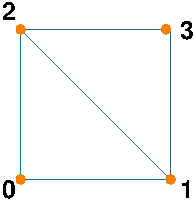
\includegraphics{tutorials/twocells/figs/twotri3-mesh}
\par\end{centering}

\caption{Mesh composed of two linear triangular cells used in the example problems.\label{fig:twotri3-mesh}}
\end{figure}



\subsection{Additional Common Information}

In addition to the mesh, the three example problems share additional
information. For problems of this type, it is generally useful to
create a file named \texttt{pylithapp.cfg} in the working directory,
since this file is read automatically every time PyLith is run. Settings
specific to a particular problem may be placed in other \texttt{.cfg}
files, as described later, and then those files are placed on the
command line. The settings contained in \texttt{pylithapp.cfg} for
this problem consist of:
\begin{description}
\item [{pylithapp.journal.info}] Settings that control the verbosity of
the output for the different components.
\item [{pylithapp.mesh\_generator}] Settings that control mesh importing,
such as the importer type, the filename, and the spatial dimension
of the mesh.
\item [{pylithapp.timedependent}] Settings that control the problem, such
as the total time, time step size, and spatial dimension.
\item [{pylithapp.timedependent.materials}] Settings that control the material
type, specify which material IDs are to be associated with a particular
material type, and give the name of the spatial database containing
the physical  properties for the material. The quadrature information
is also given.
\item [{pylithapp.petsc}] PETSc settings to use for the problem, such as
the preconditioner type.
\end{description}
All of the problems in this directory use the same material database,
as specified under 
\begin{lyxcode}
pylithapp.timedependent.materials~
\end{lyxcode}
in \texttt{pylithapp.cfg}. This information is contained in the file
\texttt{matprops.spatialdb}. Although the material model is specified
in \texttt{pylithapp.cfg}, the values for the physical properties
of the material are given in \texttt{matprops.spatialdb}. For this
example, values describing elastic plane strain material properties
are given at a single point, resulting in uniform material properties.


\subsection{Axial Displacement Example}

The first example problem is extension of the mesh along the diagonal
extending from the lower left to the upper right of the square mesh.
Parameter settings that augment those in \texttt{pylithapp.cfg} are
contained in the file \texttt{axialdisp.cfg}. These settings are:
\begin{description}
\item [{pylithapp.timedependent}] Specifies an implicit formulation for
the problem and specifies the array of boundary conditions.
\item [{pylithapp.timedependent.bc.bc}] Defines which degrees of freedom
are being constrained (x and y), gives the label (defined in \texttt{twotri3.mesh})
defining the points desired, assigns a label to the boundary condition
set, and gives the name of the spatial database with the values for
the Dirichlet boundary condition (\texttt{axialdisp.spatialdb}).
\item [{pylithapp.problem.formulation.output.output.writer}] Gives the
base filename for VTK output \\
(\texttt{axialdisp.vtk}).
\item [{pylithapp.timedependent.materials.material.output}] Gives the base
filename for state variable output files \linebreak{}
(\texttt{axialdisp-statevars.vtk}).
\end{description}
The values for the Dirichlet boundary condition are given in the file
\texttt{axialdisp.spatialdb}, as specified in \texttt{axialdisp.cfg}.
The format of all spatial database files is similar. In this case,
the desired displacement values are given at two points (lower left
and upper right). Since data are being specified at points (rather
than being uniform over the mesh, for example), the data dimension
is one.

The files containing common information (\texttt{twotri3.mesh}, \texttt{pylithapp.cfg},
\texttt{matprops.spatialdb}) along with the problem-specific files
(\texttt{axialdisp.cfg}, \texttt{axialdisp.spatialdb}) provide a complete
description of the problem, and we can then run this example by typing
\begin{lyxcode}
pylith~axialdisp.cfg
\end{lyxcode}
Once the problem has run, three files will be produced. The first
file is named \texttt{axialdisp\_t0000000.vtk}. The \texttt{t0000000}
indicates that the output is for the first (and only) time step, corresponding
to an elastic solution. This file contains mesh information as well
as displacement values at the mesh vertices. The second file is named
\texttt{axialdisp-statevars\_t0000000.vtk}. This file contains the
state variables for each cell. The default fields are the total strain
and stress fields. Since the cells are linear triangles, there is
a single quadrature point for each cell and thus a single set of stress
and strain values for each cell. The final file (\texttt{axialdisp-statevars\_info.vtk})
gives the material properties used for the problem. Since we have
not specified which properties to write, the default properties (\texttt{mu},
\texttt{lambda}, \texttt{density}) are written. All of the \texttt{.vtk}
files may be used with a number of visualization packages. If the
problem ran correctly, you should be able to generate a figure such
as Figure \vref{fig:twotri3-axial}, which was generated using ParaView.

\noindent \begin{center}
\begin{figure}
\begin{centering}
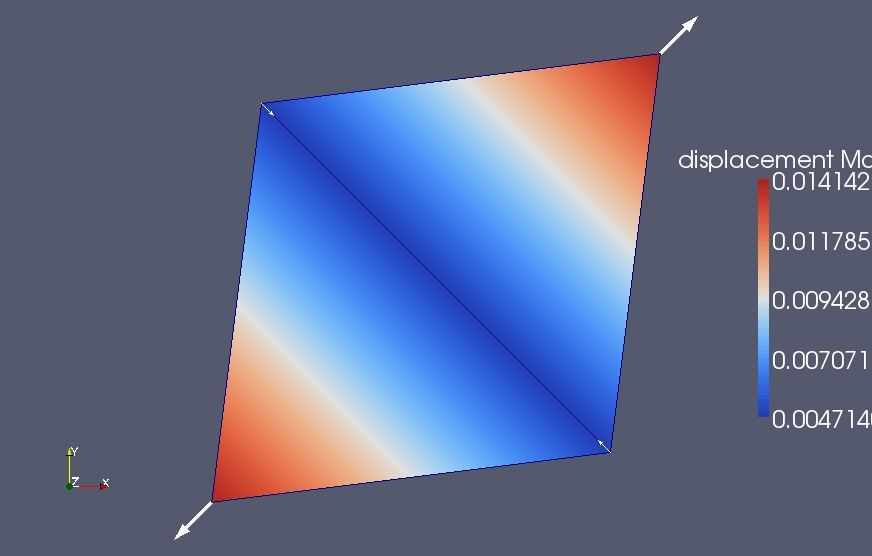
\includegraphics[scale=0.33]{tutorials/twocells/figs/twotri3-axialdisp}
\par\end{centering}

\caption{Color contours and vectors of displacement for the axial displacement
example using a mesh composed of two linear triangular cells.\label{fig:twotri3-axial}}
\end{figure}

\par\end{center}


\subsection{Shear Displacement Example}

The next example problem is shearing of the mesh in the y direction
using displacements applied along the positive and negative x boundaries.
Parameter settings that augment those in \texttt{pylithapp.cfg} are
contained in the file \texttt{sheardisp.cfg}. These settings include:
\begin{description}
\item [{pylithapp.timedependent.bc.x\_neg}] Specifies the boundary conditions
for the left side of the mesh, defining which degrees of freedom are
being constrained (x and y), giving the label (\texttt{x\_neg}, defined
in \texttt{twotri3.mesh}) defining the points desired, assigning a
label to the boundary condition set, and giving the name of the spatial
database with the values for the Dirichlet boundary condition (\texttt{sheardisp.spatialdb}).
\item [{pylithapp.timedependent.bc.x\_pos}] Specifies the boundary conditions
for the left side of the mesh, defining which degrees of freedom are
being constrained (y only), giving the label (\texttt{x\_pos}, defined
in \texttt{twotri3.mesh}) defining the points desired, assigning a
label to the boundary condition set, and giving the name of the spatial
database with the values for the Dirichlet boundary condition (\texttt{sheardisp.spatialdb}).
\end{description}
The files containing common information (\texttt{twotri3.mesh}, \texttt{pylithapp.cfg},
\texttt{matprops.spatialdb}) along with the problem-specific files
(\texttt{sheardisp.cfg}, \texttt{sheardisp.spatialdb}) provide a complete
description of the problem, and we can then run this example by typing
\begin{lyxcode}
pylith~sheardisp.cfg
\end{lyxcode}
Once the problem has run, three files will be produced as in the previous
example. If the problem ran correctly, you should be able to generate
a figure such as Figure \vref{fig:twotri-shear}, which was generated
using ParaView.

\noindent \begin{center}
\begin{figure}
\begin{centering}
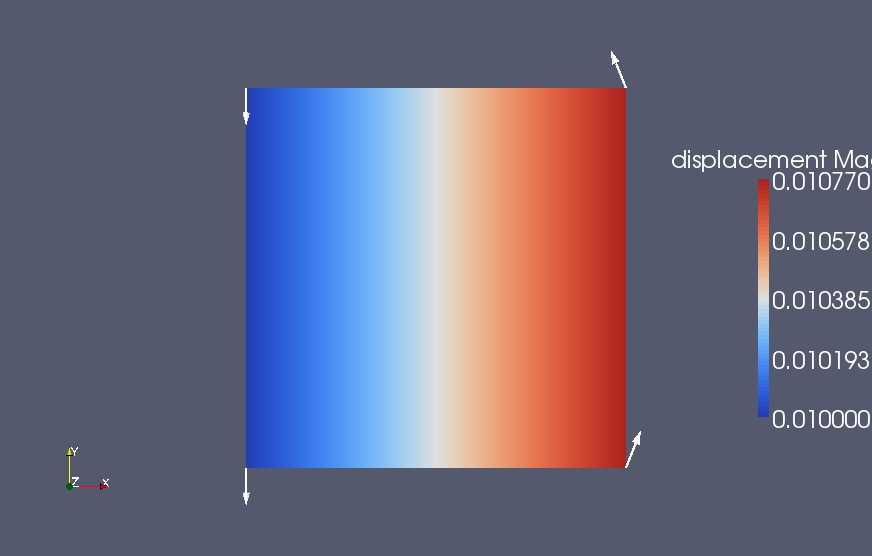
\includegraphics[scale=0.33]{tutorials/twocells/figs/twotri3-sheardisp}
\par\end{centering}

\caption{Color contours and vectors of displacement for the shear displacement
example using a mesh composed of two linear triangular cells.\label{fig:twotri-shear}}
\end{figure}

\par\end{center}


\subsection{Kinematic Fault Slip Example}

The next example problem is left-lateral fault slip applied between
the two triangular cells using kinematic cohesive cells. The lower
left and upper right boundaries are held fixed in the x and y directions.
Parameter settings that augment those in \texttt{pylithapp.cfg} are
contained in the file \texttt{dislocation.cfg}. The solution corresponds
to rigid body rotation of each triangular cell. As a result, the tractions
on the fault are zero. These settings include:
\begin{description}
\item [{pylithapp.journal.info}] Turns on journaling for 1D quadrature
(used for 2D faults) and for cohesive kinematic faults.
\item [{pylithapp.timedependent.bc.bc}] Defines which degrees of freedom
are being constrained (x and y), gives the label (defined in \texttt{twotri3.mesh})
defining the points desired, and assigns a label to the boundary condition
set. In this case, rather than specifying a spatial database file
with the values for the Dirichlet boundary condition, the default
database (ZeroDispDB) for Dirichlet boundary conditions is used, which
sets the displacements to zero.
\item [{pylithapp.timedependent.interfaces}] Gives the label (defined in
\texttt{twotri3.mesh}) defining the points on the fault, provides
quadrature information, and then gives database names for material
properties (needed for conditioning), fault slip, peak fault slip
rate, and fault slip time.
\item [{pylithapp.timedependent.interfaces.fault.output.writer}] Gives
the base filename for cohesive cell output files \linebreak{}
(\texttt{dislocation-fault.vtk}).
\end{description}
Rather than specifying the displacement boundary conditions in a spatial
database file, we use the default behavior for Dirichlet boundary
conditions, which is a uniform, constant displacement of zero.

The fault example requires three additional database files that were
not needed for the simple displacement examples. The first file (\texttt{dislocation\_slip.spatialdb})
specifies 0.01 m of left-lateral fault slip for the entire fault.
The data dimension is zero since the same data are applied to all
points in the set. The default slip time function is a step-function,
so we also must provide the time at which slip begins. The elastic
solution is associated with advancing from $t=-dt$ to $t=0$, so
we set the slip initiation time for the step-function to 0 in \texttt{dislocation\_sliptime.spatialdb}.

The files containing common information (\texttt{twotri3.mesh}, \texttt{pylithapp.cfg},
\texttt{matprops.spatialdb}) along with the problem-specific files
(\texttt{\small{}dislocation.cfg}{\small{}, }\texttt{\small{}dislocation\_slip.spatialdb}{\small{},
}\texttt{\small{}}~\linebreak{}
\texttt{\small{}dislocation\_sliptime.spatialdb}) provide a complete
description of the problem, and we can then run this example by typing
\begin{lyxcode}
pylith~dislocation.cfg
\end{lyxcode}
Once the problem has run, five files are produced. In addition to
the files produced in the previous two examples, this example produces
two files associated with the fault interface. The file \texttt{dislocation-fault\_t0000000.vtk}
gives the fault slip for each vertex on the fault along with the computed
traction change for the cohesive cell. The file \texttt{dislocation-fault\_info.vtk}
provides information such as the normal direction, final slip, and
slip time for each vertex on the fault. If the problem ran correctly,
you should be able to generate a figure such as Figure \vref{fig:twotri-disloc},
which was generated using ParaView.

\noindent \begin{center}
\begin{figure}
\begin{centering}
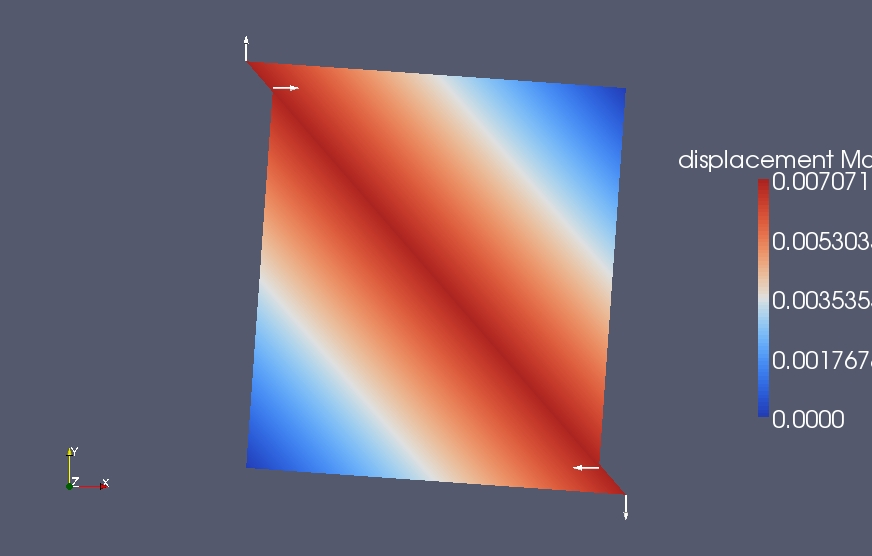
\includegraphics[scale=0.33]{tutorials/twocells/figs/twotri3-dislocation}
\par\end{centering}

\caption{Color contours and vectors of displacement for the kinematic fault
example using a mesh composed of two linear triangular cells.\label{fig:twotri-disloc}}
\end{figure}

\par\end{center}
 
\section{\label{sec:Tutorial-Two-quad4}Tutorial Using Two Quadrilaterals}

PyLith features discussed in this tutorial:
\begin{itemize}
\item Quasi-static solution
\item Mesh ASCII format
\item Dirichlet boundary conditions
\item Neumann boundary conditions
\item Kinematic fault interface conditions
\item Plane strain linearly elastic material
\item VTK output
\item Bilinear quadrilateral cells
\item SimpleDB spatial database
\item ZeroDispDB spatial database
\end{itemize}
All of the files necessary to run the examples are contained in the
directory \texttt{examples/twocells/twoquad4.}


\subsection{Overview}

This tutorial is another simple 2D example of a quasi-static finite
element problem. It is a mesh composed of two bilinear quadrilaterals
subject to displacement or traction boundary conditions, assuming
plane-strain linear elastic behavior. Due to the simple geometry of
the problem, the mesh may be constructed by hand, using PyLith mesh
ASCII format to describe the mesh. In this tutorial, we will walk
through the steps necessary to construct, run, and view four problems
that use the same mesh. In addition to this manual, each of the files
for the example problem includes extensive comments.


\subsection{Mesh Description}

The mesh consists of two square cells with edge lengths of one unit
forming a regular region (Figure \vref{fig:twoquad4-mesh}). The mesh
geometry and topology are described in the file \texttt{twoquad4.mesh},
which is in PyLith mesh ASCII format. This file describes the dimensionality
of the problem (in this case 2D), the coordinates of the vertices
(nodes), the vertices composing each cell (element), the material
ID to be associated with each cell, and then provides groups of vertices
that may be used to define faults or surfaces to which boundary conditions
may be applied.

\noindent \begin{center}
\begin{figure}
\begin{centering}
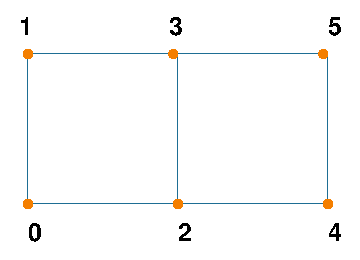
\includegraphics{tutorials/twocells/figs/twoquad4-mesh}
\par\end{centering}

\caption{Mesh composed of two bilinear quadrilateral cells used for the example
problems.\label{fig:twoquad4-mesh}}
\end{figure}

\par\end{center}


\subsection{Additional Common Information}

In addition to the mesh, the four example problems share additional
information. As in the previous examples, we place this information
in \texttt{pylithapp.cfg}, since this file is read automatically every
time PyLith is run. Settings specific to a particular problem may
be placed in other \texttt{.cfg} files, as described later, and then
those files are placed on the command line.


\subsection{Axial Displacement Example}

The first example problem is extension of the mesh along the x axis.
Parameter settings that override or augment those in \texttt{pylithapp.cfg}
are contained in the file \texttt{axialdisp.cfg}. These include:
\begin{description}
\item [{pylithapp.timedependent.bc.x\_neg}] Specifies the boundary conditions
for the left side of the mesh, defining which degrees of freedom are
being constrained (x), giving the label (defined in \texttt{twoquad4.mesh})
defining the points desired, assigning a label to the boundary condition
set, and giving the name of the spatial database with the values for
the Dirichlet boundary condition (\texttt{axialdisp.spatialdb}).
\item [{pylithapp.timedependent.bc.x\_pos}] Specifies the boundary conditions
for the right side of the mesh, defining which degrees of freedom
are being constrained (x), giving the label (defined in \texttt{twoquad4.mesh})
defining the points desired, assigning a label to the boundary condition
set, and giving the name of the spatial database defining the boundary
conditions (\texttt{axialdisp.spatialdb}).
\item [{pylithapp.timedependent.bc.y\_neg}] Specifies the boundary conditions
for the bottom two corners of the mesh, defining which degrees of
freedom are being constrained (y), giving the label (defined in \texttt{twoquad4.mesh})
defining the points desired, assigning a label to the boundary condition
set, and giving the name of the spatial database with the values for
the Dirichlet boundary condition (\texttt{axialdisp.spatialdb}).
\end{description}
The values for the Dirichlet boundary condition are given in the file
\texttt{axialdisp.spatialdb}, as specified in \texttt{axialdisp.cfg}.
Because the data are being specified using two control points with
a linear variation in the values between the two (rather than being
uniform over the mesh, for example), the data dimension is one.

The files containing common information (\texttt{twoquad4.mesh}, \texttt{pylithapp.cfg},
\texttt{matprops.spatialdb}) along with the problem-specific files
(\texttt{axialdisp.cfg}, \texttt{axialdisp.spatialdb}) provide a complete
description of the problem, and we can then run this example by typing
\begin{lyxcode}
pylith~axialdisp.cfg
\end{lyxcode}
As in the two triangle axial displacement example, three files will
be produced. If the problem ran correctly, you should be able to produce
a figure such as Figure \vref{fig:twoquad4-axial}, which was generated
using ParaView.

\noindent \begin{center}
\begin{figure}[t]
\begin{centering}
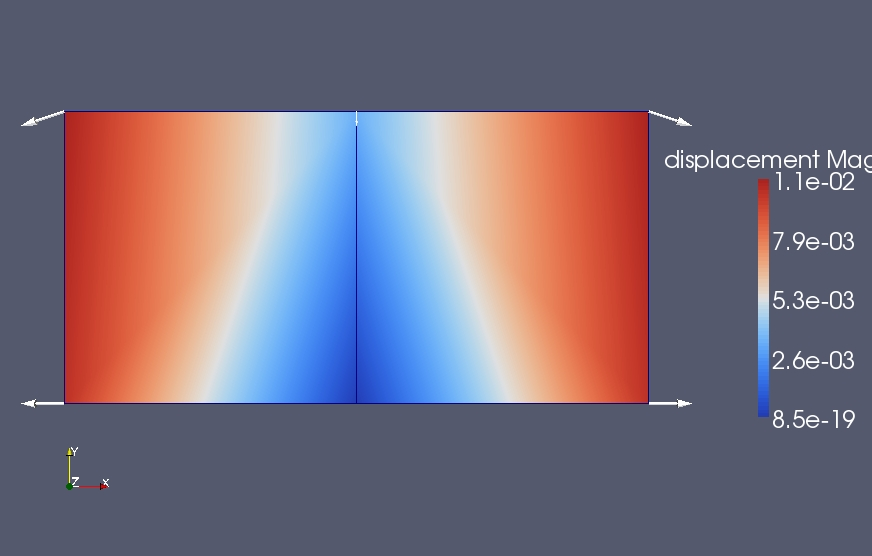
\includegraphics[scale=0.33]{tutorials/twocells/figs/twoquad4-axialdisp}
\par\end{centering}

\caption{Color contours and vectors of displacement for the axial displacement
example using a mesh composed of two bilinear quadrilateral cells.\label{fig:twoquad4-axial}}
\end{figure}

\par\end{center}


\subsection{Shear Displacement Example}

The next example problem is shearing of the mesh in the y direction
using displacements applied along the positive and negative x boundaries.
Parameter settings that override or augment those in \texttt{pylithapp.cfg}
are contained in the file \texttt{sheardisp.cfg}. These include:
\begin{description}
\item [{pylithapp.timedependent.bc.x\_neg}] Specifies the boundary conditions
for the left side of the mesh, defining which degrees of freedom are
being constrained (x and y), giving the label (\texttt{x\_neg}, defined
in \texttt{twoquad4.mesh}) defining the points desired, assigning
a label to the boundary condition set, and giving the name of the
spatial database with the values for the Dirichlet boundary condition
(\texttt{sheardisp.spatialdb}).
\item [{pylithapp.timedependent.bc.x\_pos}] Specifies the boundary conditions
for the left side of the mesh, defining which degrees of freedom are
being constrained (y only), giving the label (\texttt{x\_pos}, defined
in \texttt{twoquad4.mesh}) defining the points desired, assigning
a label to the boundary condition set, and giving the name of the
spatial database with the values for the Dirichlet boundary condition
(\texttt{sheardisp.spatialdb}).
\end{description}
The values for the Dirichlet boundary conditions are described in
the file \texttt{sheardisp.spatialdb}, as specified in \texttt{sheardisp.cfg}.
In this case, the desired displacement values are given at two control
points, corresponding to the two edges we want to constrain. Since
data are being specified at two points with a linear variations in
the values between the points (rather than being uniform over the
mesh, for example), the data dimension is one.

The files containing common information (\texttt{twoquad4.mesh}, \texttt{pylithapp.cfg},
\texttt{matprops.spatialdb}) along with the problem-specific files
(\texttt{sheardisp.cfg}, \texttt{sheardisp.spatialdb}) provide a complete
description of the problem, and we can then run this example by typing
\begin{lyxcode}
pylith~sheardisp.cfg
\end{lyxcode}
As in the previous example, three files will be produced. If the problem
ran correctly, you should be able to produce a figure such as Figure
\vref{fig:twoquad4-shear}, which was generated using ParaView.

\begin{figure}
\begin{centering}
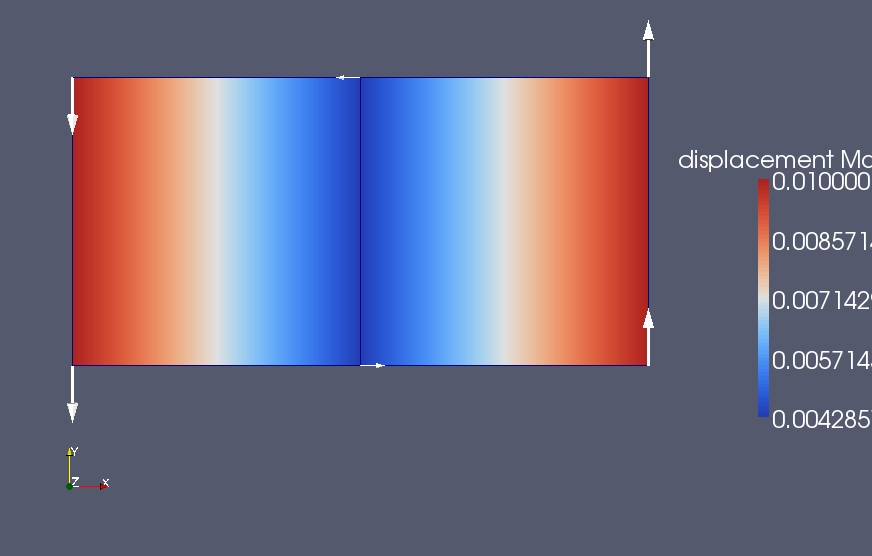
\includegraphics[scale=0.33]{tutorials/twocells/figs/twoquad4-sheardisp}
\par\end{centering}

\caption{Color contours and vectors of displacement for the shear displacement
example using a mesh composed of two bilinear quadrilateral cells.\label{fig:twoquad4-shear}}
\end{figure}



\subsection{Kinematic Fault Slip Example}

The next example problem is a left-lateral fault slip applied between
the two square cells using kinematic cohesive cells. The left and
right boundaries are held fixed in the x and y directions. Parameter
settings that override or augment those in \texttt{pylithapp.cfg}
are contained in the file \texttt{dislocation.cfg}. These settings
include:
\begin{description}
\item [{pylithapp.timedependent.bc.x\_neg}] Specifies the boundary conditions
for the left side of the mesh, defining which degrees of freedom are
being constrained (x and y), giving the label (\texttt{x\_neg}, defined
in \texttt{twoquad4.mesh}) defining the points desired, and assigning
a label to the boundary condition set. Instead of specifying a spatial
database file for the values of the Dirichlet boundary condition,
we use the default spatial database (ZeroDispDB) for the Dirichlet
boundary condition, which sets the displacements to zero for all time.
\item [{pylithapp.timedependent.bc.x\_pos}] Specifies the boundary conditions
for the right side of the mesh, defining which degrees of freedom
are being constrained (x and y), giving the label (\texttt{x\_neg},
defined in \texttt{twoquad4.mesh}) defining the points desired, and
assigning a label to the boundary condition set. We use the ZeroDispDB
for this boundary condition as well, which sets the displacements
to zero for all time.
\item [{pylithapp.timedependent.interfaces}] Gives the label (defined in
\texttt{twoquad4.mesh}) defining the points on the fault, provides
quadrature information, and then gives database names for material
properties (needed for conditioning), fault slip, peak fault slip
rate, and fault slip time.
\end{description}
The fault example requires three additional database files that were
not needed for the simple displacement examples. The first file (\texttt{dislocation\_slip.spatialdb})
specifies 0.01 m of left-lateral fault slip for the entire fault.
The data dimension is zero since the same data are applied to all
points in the set. The default slip time function is a step-function,
so we also must provide the time at which slip begins. The elastic
solution is associated with advancing from $t=-dt$ to $t=0$, so
we set the slip initiation time for the step-function to 0 in \texttt{dislocation\_sliptime.spatialdb}.

The files containing common information (\texttt{twoquad4.mesh}, \texttt{pylithapp.cfg},
\texttt{matprops.spatialdb}) along with the problem-specific files
(\texttt{\small{}dislocation.cfg}{\small{}, }\texttt{\small{}dislocation\_slip.spatialdb}{\small{},
}\texttt{\small{}}~\linebreak{}
\texttt{\small{}dislocation\_sliptime.spatialdb}) provide a complete
description of the problem, and we can then run this example by typing
\begin{lyxcode}
pylith~dislocation.cfg
\end{lyxcode}
The addition of a fault results in two additional output files (as
in the two triangle fault example), \texttt{}~\linebreak{}
\texttt{dislocation-fault\_t0000000.vtk} and \texttt{dislocation-fault\_info.vtk}.
These files provide output of fault slip, change in tractions, and
diagnostic information such as the normal direction, final slip, and
slip time for each vertex on the fault. If the problem ran correctly,
you should be able to produce a figure such as Figure \vref{fig:twoquad4-disloc},
which was generated using ParaView.

\begin{figure}
\begin{centering}
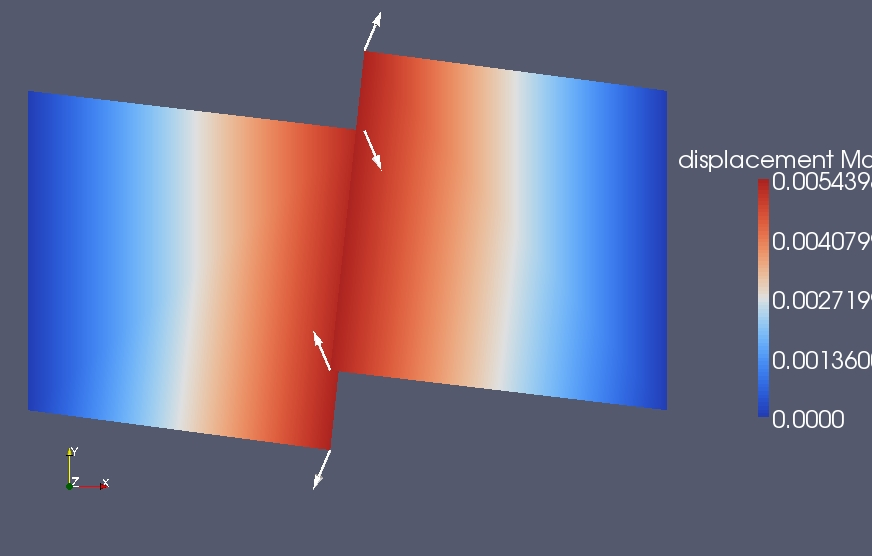
\includegraphics[scale=0.33]{tutorials/twocells/figs/twoquad4-dislocation}
\par\end{centering}

\caption{Color contours and vectors of displacement for the kinematic fault
example using a mesh composed of two bilinear quadrilateral cells.\label{fig:twoquad4-disloc}}
\end{figure}



\subsection{\label{sub:Tutorial-twoquad4-traction}Axial Traction Example}

The fourth example demonstrates the use of Neumann (traction) boundary
conditions. Constant tractions are applied to the right edge of the
mesh, while displacements normal to the boundaries are held fixed
along the left and bottom edges of the mesh. Parameter settings that
override or augment those in \texttt{pylithapp.cfg} are contained
in the file \texttt{axialtract.cfg}. These settings include:
\begin{description}
\item [{pylithapp.timedependent}] Specifies an implicit formulation for
the problem and specifies the array of boundary conditions. The boundary
condition type for \texttt{x\_pos} is explicitly set to \texttt{Neumann},
since the default boundary condition type is \texttt{Dirichlet}.
\item [{pylithapp.timedependent.bc.x\_neg}] Specifies the boundary conditions
for the left side of the mesh, defining which degrees of freedom are
being constrained (x) and giving the label (defined in \texttt{twoquad4.mesh})
defining the points desired. In this case, rather than specifying
a spatial database file with values for the Dirichlet boundary conditions,
we use the default spatial database (ZeroDispDB) for the Dirichlet
boundary condition, which sets the displacements to zero for all time.
\item [{pylithapp.timedependent.bc.x\_pos}] Specifies the Neumann boundary
conditions for the right side of the mesh, giving the label (defined
in \texttt{twoquad4.mesh}) defining the points desired, assigning
a label to the boundary condition set, and giving the name of the
spatial database with the traction vectors for the Neumann boundary
condition (\texttt{axialtract.spatialdb}).
\item [{pylithapp.timedependent.bc.y\_neg}] Specifies the boundary conditions
for the bottom two corners of the mesh, defining which degrees of
freedom are being constrained (y) and giving the label (defined in
\texttt{twoquad4.mesh}) defining the points desired. In this case,
we again use the ZeroDispDB, which sets the displacements to zero
for all time.
\item [{pylithapp.problem.formulation.output.output.writer}] Gives the
base filename for VTK output \\
(\texttt{axialtract.vtk}).
\item [{pylithapp.timedependent.bc.x\_pos.output}] Gives the field to be
output for the \texttt{x\_pos} boundary (\texttt{tractions}), and
gives the base filename for \texttt{x\_pos} boundary output (\texttt{axialtract-tractions.vtk}).
\end{description}
The traction vectors for the Neumann boundary conditions are given
in the file \texttt{axialtract.spatialdb}, as specified in \texttt{axialtract.cfg}.
The files containing common information (\texttt{twoquad4.mesh}, \texttt{pylithapp.cfg},
\texttt{matprops.spatialdb}) along with the problem-specific files
(\texttt{axialtract.cfg}, \texttt{axialtract.spatialdb}) provide a
complete description of the problem, and we can then run this example
by typing
\begin{lyxcode}
pylith~axialtract.cfg
\end{lyxcode}
Once the problem has run, six files will be produced. This includes
the five files as in the previous example plus \texttt{axialtract-tractions\_info.vtk},
which gives the \texttt{x} and \texttt{y} components of traction applied
at each integration point. If the problem ran correctly, you should
be able to produce a figure such as Figure \vref{fig:twoquad4-axialtract},
which was generated using ParaView. The results may be compared against
the analytical solution derived in Section \vref{sub:Analytical-Constant-Traction}.

\begin{figure}
\begin{centering}
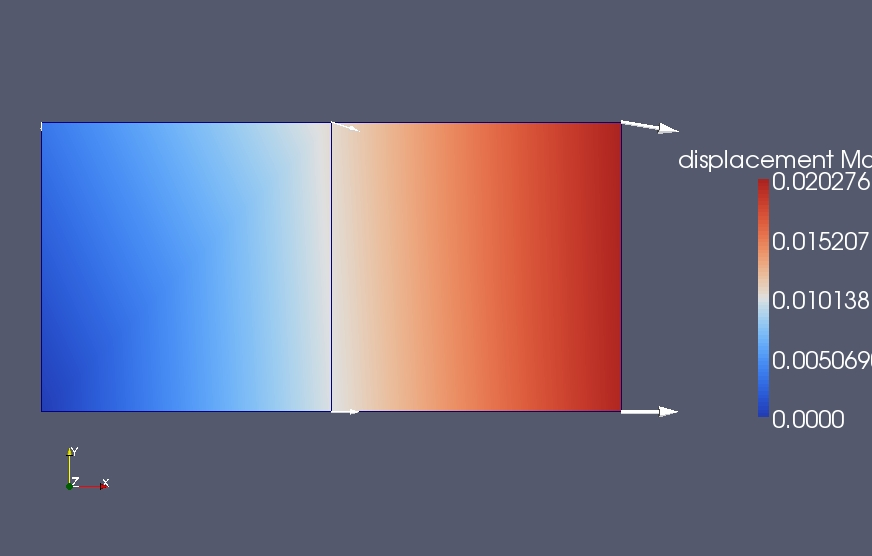
\includegraphics[scale=0.33]{tutorials/twocells/figs/twoquad4-axialtract}
\par\end{centering}

\caption{Color contours and vectors of displacement for the axial traction
example using a mesh composed of two bilinear quadrilateral cells.\label{fig:twoquad4-axialtract}}
\end{figure}


\section{Example Using Two Tetrahedra}
\label{sec:example:twotet4}

PyLith features discussed in this example:
\begin{itemize}
\item Quasi-static solution
\item Mesh ASCII format
\item Dirichlet boundary conditions
\item Kinematic fault interface conditions
\item Linearly elastic isotropic material
\item VTK output
\item Linear tetrahedral cells
\item SimpleDB spatial database
\item ZeroDispDB spatial database
\end{itemize}
All of the files necessary to run the examples are contained in the
directory \filename{examples/twocells/twotet4.}


\subsection{Overview}

This example is a simple 3D example of a quasi-static finite element
problem. It is a mesh composed of two linear tetrahedra subject to
displacement boundary conditions, and is probably the simplest example
of a 3D elastic problem. Due to the simple geometry of the problem,
the mesh may be constructed by hand, using PyLith mesh ASCII format.
In this example, we will walk through the steps necessary to
construct, run, and view two problems that use the same mesh. In
addition to this manual, each of the files for the example problem
includes extensive comments.


\subsection{Mesh Description}

The mesh consists of two tetrahedra forming a pyramid shape (Figure
\vref{fig:twotet4-mesh}). The mesh geometry and topology is described
in the file \filename{twotet4.mesh}, which is in PyLith mesh ASCII
format.

\begin{figure}
  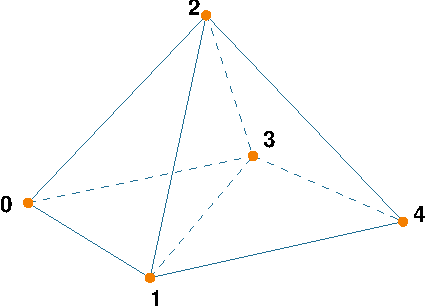
\includegraphics{examples/figs/twotet4-mesh}
  \caption{Mesh composed of two linear tetrahedral cells used for example problems.}
  \label{fig:twotet4-mesh}
\end{figure}


\subsection{Additional Common Information}

In addition to the mesh, the two example problems share additional
information, which we place in \filename{pylithapp.cfg}.


\subsection{Axial Displacement Example}

The first example problem is extension of the mesh along the diagonal,
extending along the base of the pyramid between two opposing vertices.
Parameter settings that override or augment those in \filename{pylithapp.cfg}
are contained in the file \filename{axialdisp.cfg}. These settings include:
\begin{inventory}
  \facilityitem{pylithapp.timedependent.bc.bc}{Defines which degrees of freedom
    are being constrained (\texttt{x}, \texttt{y}, and \texttt{z}), gives
    the label (defined in \filename{twotet4.mesh}) defining the points desired,
    assigns a label to the boundary condition set, and gives the name
    of the spatial database defining the boundary conditions (\filename{axialdisp.spatialdb}).}
\end{inventory}
The values for the Dirichlet boundary conditions are described in
the file \filename{axialdisp.spatialdb}, as specified in \filename{axialdisp.cfg}.
Because data are being specified using two control points (rather
than being uniform over the mesh), the data dimension is one.

The files containing common information (\filename{twotet4.mesh},
\filename{pylithapp.cfg}, \filename{matprops.spatialdb}) along with
the problem-specific files (\filename{axialdisp.cfg},
\filename{axialdisp.spatialdb}) provide a complete description of the
problem, and we can then run this example by typing
\begin{shell}
$ pylith axialdisp.cfg
\end{shell}
If the problem ran correctly, you should be able to produce a figure
such as Figure \vref{fig:twotet4-axial}, which was generated using
ParaView.

\begin{figure}
  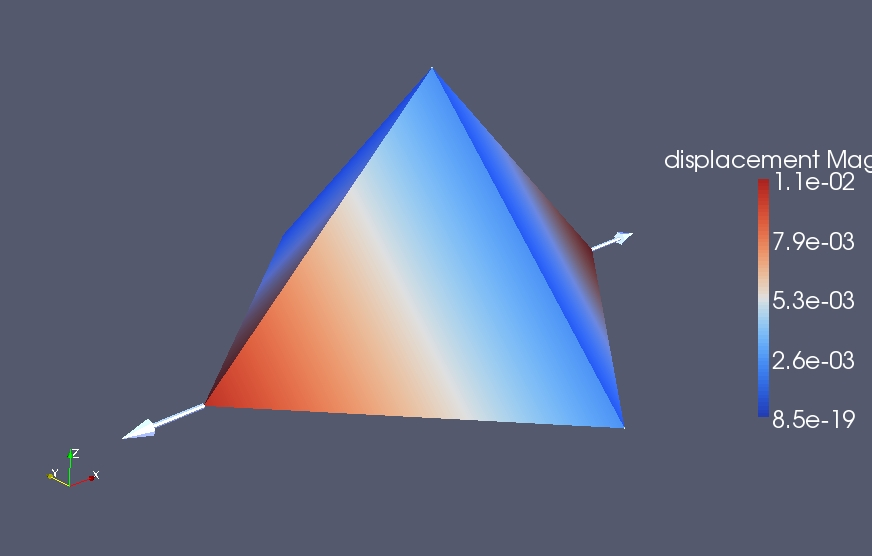
\includegraphics[scale=0.33]{examples/figs/twotet4-axialdisp}
  \caption{Color contours and vectors of displacement for the axial displacement
    example using a mesh composed of two linear tetrahedral cells.}
  \label{fig:twotet4-axial}
\end{figure}


\subsection{Kinematic Fault Slip Example}

The next example problem is a left-lateral fault slip applied between
the two tetrahedral cells using kinematic cohesive cells. The vertices
away from the fault are held fixed in the \texttt{x}, \texttt{y},
and \texttt{z} directions. Parameter settings that override or augment
those in \filename{pylithapp.cfg} are contained in the file \filename{dislocation.cfg}.
These settings include:
\begin{inventory}
  \facilityitem{pylithapp.timedependent.bc.bc}{Defines which degrees of freedom
    are being constrained (\texttt{x}, \texttt{y}, and \texttt{z}), gives
    the label (defined in \filename{twotet4.mesh}) defining the points desired,
    and assigns a label to the boundary condition set. Rather than specifying
    a spatial database file to define the boundary conditions, we use
    the default spatial database (ZeroDispDB) for the Dirichlet boundary
    condition, which sets the displacements to zero.}
  \facilityitem{pylithapp.timedependent.interfaces}{Gives the label (defined in
    \filename{twotet4.mesh}) defining the points on the fault, provides
    quadrature information, and then gives database names for material
    properties (needed for conditioning), fault slip, peak fault slip
    rate, and fault slip time.}
\end{inventory}
The fault example requires three additional database files that were
not needed for the simple displacement examples. The first file
(\filename{dislocation\_slip.spatialdb}) specifies 0.01 m of
left-lateral fault slip for the entire fault.  The data dimension is
zero since the same data are applied to all points in the set. The
default slip time function is a step-function, so we also must provide
the time at which slip begins. The elastic solution is associated with
advancing from $t=-dt$ to $t=0$, so we set the slip initiation time
for the step-function to 0 in
\filename{dislocation\_sliptime.spatialdb}.

The files containing common information (\filename{twotet4.mesh}, \filename{pylithapp.cfg},
\filename{matprops.spatialdb}) along with the problem-specific files
(\filename{dislocation.cfg, dislocation\_slip.spatialdb},
\filename{dislocation\_sliptime.spatialdb}) provide a complete description
of the problem, and we can then run this example by typing
\begin{shell}
$ pylith dislocation.cfg
\end{shell}
If the problem ran correctly, you should be able to generate a figure
such as Figure \vref{fig:twotet4-disloc}, which was generated using
ParaView.

\begin{figure}
  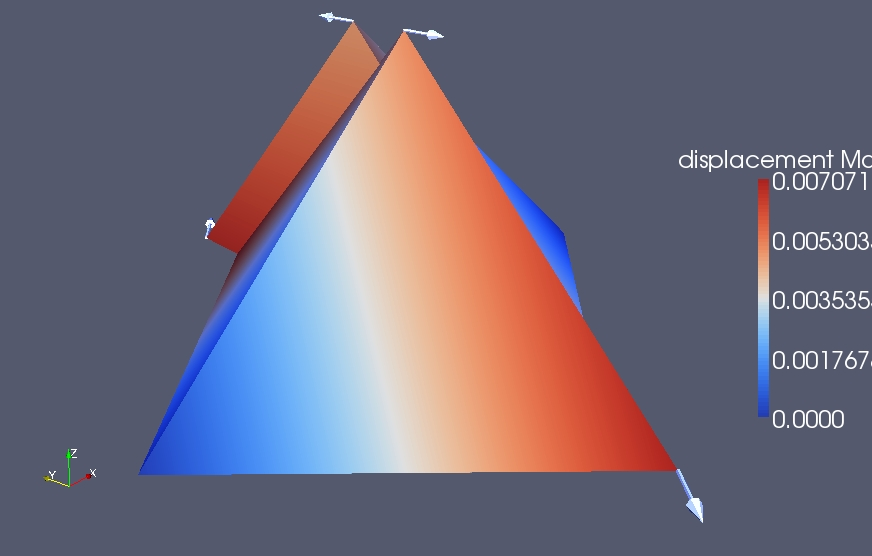
\includegraphics[scale=0.33]{examples/figs/twotet4-dislocation}
  \caption{Color contours and vectors of displacement for the kinematic fault
    example using a mesh composed of two linear tetrahedral cells.}
  \label{fig:twotet4-disloc}
\end{figure}


% End of file
\section{Example Using Two Hexahedra}
\label{sec:example:twohex8}

PyLith features discussed in this example:
\begin{itemize}
\item Quasi-static solution
\item Mesh ASCII format
\item Dirichlet boundary conditions
\item Kinematic fault interface conditions
\item Maxwell viscoelastic material
\item VTK output
\item Trilinear hexahedral cells
\item SimpleDB spatial database
\item ZeroDispDB spatial database
\item UniformDB spatial database
\item Filtering of cell output fields
\end{itemize}
All of the files necessary to run the examples are contained in the
directory \filename{examples/twocells/twohex8.}


\subsection{Overview}

This example is a simple 3D example of a quasi-static finite element
problem. It is a mesh composed of two trilinear hexahedra subject
to displacement boundary conditions. One primary difference between
this example and the example with two tetrahedra is that we use a
Maxwell viscoelastic material model, and run the model for 10 time
steps of 0.1 year each. Due to the simple geometry of the problem,
the mesh may be constructed by hand, using PyLith mesh ASCII format
to describe the mesh. In this example, we will walk through the steps
necessary to construct, run, and view three problems that use the
same mesh. In addition to this manual, each of the files for the example
problems includes extensive comments.


\subsection{Mesh Description}

The mesh consists of two hexahedra forming a rectangular prism (Figure
\vref{fig:twohex8-mesh}). The mesh geometry and topology are described
in the file \filename{twohex8.mesh}, which is in PyLith mesh ASCII format.

\begin{figure}
  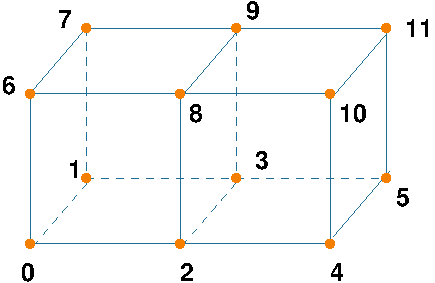
\includegraphics{examples/figs/twohex8-mesh}
  \caption{Mesh composed of two trilinear hexahedral cells used for
    the example problems.}
  \label{fig:twohex8-mesh}
\end{figure}


\subsection{Additional Common Information}

In addition to the mesh, the three example problems share additional
information, which we place in \filename{pylithapp.cfg}. Note that in
this example we make use of the UniformDB spatial database, rather
than the SimpleDB implementation used to specify the physical properties
in the other example problems. For simple distributions of material
properties (or boundary conditions), this implementation is often
easier to use. Examining \filename{pylithapp.cfg}, we specify the material
information with the following set of parameters:
\begin{cfg}
<h>[pylithapp.timedependent.materials]</h>
<f>material</f> = pylith.materials.MaxwellIsotropic3D

<h>[pylithapp.timedependent.materials.material]</h>
<p>label</p> = viscoelastic material
<p>id</p> = 1
<f>db</pf> = spatialdata.spatialdb.UniformDB
<p>db.values</p> = [vp, vs, density, viscosity]
<p>db.data</p> = [5773.502691896258*m/s, 3333.333333333333*m/s, 2700.0*kg/m**3, 1.0e18*Pa*s]

<f>quadrature.cell</f> = pylith.feassemble.FIATLagrange
<p>quadrature.cell.dimension</p> = 3
\end{cfg}

\subsection{Axial Displacement Example}

The first example problem is extension of the mesh along the long
axis of the prism. Parameter settings that override or augment those
in \filename{pylithapp.cfg} are contained in the file \filename{axialdisp.cfg}.
These settings include:
\begin{inventory}
  \facilityitem{pylithapp.timedependent.bc.x\_neg}{Defines which degrees of freedom
    are being constrained (x, y, and z), gives the label (\facility{x\_neg},
    defined in \filename{twohex8.mesh}) defining the points desired, assigns
    a label to the boundary condition set, and gives the name of the spatial
    database with the values for the Dirichlet boundary conditions (\filename{axialdisp.spatialdb}).}
  \facilityitem{pylithapp.timedependent.bc.x\_pos}{Defines which degrees of freedom
    are being constrained (x, y, and z), gives the label (\facility{x\_pos},
    defined in \filename{twohex8.mesh}) defining the points desired, assigns
    a label to the boundary condition set, and gives the name of the spatial
    database with the values for the Dirichlet boundary conditions (\filename{axialdisp.spatialdb}).}
  \facilityitem{pylithapp.timedependent.materials.material.output}{Defines the
    filter to be used when writing cell state variables (average over
    the quadrature points of the cell), specifies which state variables
    and properties to output, gives the base filename for state variable
    output files, and defines the format to use when defining the output
    filenames for each time step.}
\end{inventory}
The values for the Dirichlet boundary conditions are given in the
file \filename{axialdisp.spatialdb}, as specified in \filename{axialdisp.cfg}.
Since data are being specified using two control points (rather than
being uniform over the mesh, for example), the data dimension is one.
Note that since we are using a Maxwell viscoelastic model, we request
that additional state variables and properties be output:
\begin{cfg}
<h>[pylithapp.timedependent.materials.material.output]</h>
<p>cell_data_fields</p> = [total_strain, viscous_strain, stress]
<p>cell_info_fields</p> = [mu, lambda, density, maxwell_time]
\end{cfg}
The files containing common information (\filename{twohex8.mesh},
\filename{pylithapp.cfg}) along with the problem-specific files
(\filename{axialdisp.cfg}, \filename{axialdisp.spatialdb}) provide a
complete description of the problem, and we can then run this example
by typing
\begin{shell}
$$ pylith axialdisp.cfg
\end{shell}
Once the problem has run, two sets of files will be produced, along
with one additional file. The first set will have filenames such as
\filename{axialdisp\_txxxx.vtk}, where \filename{xxxx} is the time for
which output has been produced. In \filename{axialdisp.cfg} we specify
that the time stamp should be normalized by a value of 1.0 years and
the time stamp should be of the form \filename{xxx.x} (recall that the
decimal point is removed in the filename). As a result, the filenames
contain the time in tenths of a year. These files will contain mesh
information as well as displacement values for the mesh vertices at
the given time. The second set of files will have names such as
\filename{axialdisp-statevars\_txxxx.vtk}, where \filename{xxxx} is
the time in tenths of a year (as above) for which output has been
produced. These files contain the state variables for each cell at the
given time. The default fields are the total strain and stress fields;
however, we have also requested the viscous strains. As specified in
\filename{axialdisp.cfg}, these values are averaged over each
cell. The final file (\filename{axialdisp-statevars\_info.vtk}) gives
the material properties used for the problem. We have requested all of
the properties available for this material model (\texttt{mu},
\texttt{lambda}, \texttt{density}, \texttt{maxwell\_time}). If the
problem ran correctly, you should be able to produce a figure such as
Figure \vref{fig:twohex8-axial}, which was generated using ParaView.

\begin{figure}
  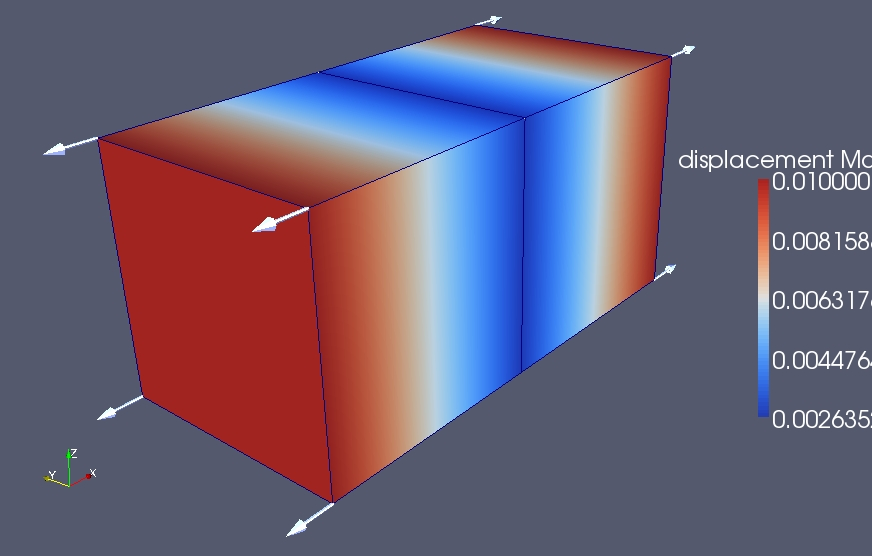
\includegraphics[scale=0.33]{examples/figs/twohex8-axialdisp}
  \caption{Color contours and vectors of displacement for the axial displacement
    example using a mesh composed of two trilinear hexahedral cells.}
  \label{fig:twohex8-axial}
\end{figure}


\subsection{Shear Displacement Example}

The second example problem is shearing of the mesh in the y direction.
Parameter settings that override or augment those in \filename{pylithapp.cfg}
are contained in the file \filename{sheardisp.cfg}. These settings include:
\begin{inventory}
  \facilityitem{pylithapp.timedependent.bc.x\_neg}{Defines which degrees of freedom
    are being constrained (x, y, and z), gives the label (\facility{x\_neg},
    defined in \filename{twohex8.mesh}) defining the points desired, assigns
    a label to the boundary condition set, and gives the name of the spatial
    database with the values for the Dirichlet boundary conditions (\filename{sheardisp.spatialdb}).}
  \facilityitem{pylithapp.timedependent.bc.x\_pos}{Defines which degrees of freedom
    are being constrained (x, y, and z), gives the label (\facility{x\_pos},
    defined in \filename{twohex8.mesh}) defining the points desired, assigns
    a label to the boundary condition set, and gives the name of the spatial
    database with the values for the Dirichlet boundary conditions (\filename{sheardisp.spatialdb}).}
\end{inventory}
The values for the Dirichlet boundary conditions are given in the
file \filename{sheardisp.spatialdb}, as specified in \filename{sheardisp.cfg}.
Data are being specified at two control points (rather than being
uniform over the mesh, for example), so the data dimension is one.
The files containing common information (\filename{twohex8.mesh}, \filename{pylithapp.cfg})
along with the problem-specific files (\filename{sheardisp.cfg}, \filename{sheardisp.spatialdb})
provide a complete description of the problem, and we can then run
this example by typing
\begin{shell}
$$ pylith sheardisp.cfg
\end{shell}
If the problem ran correctly, you should be able to generate a figure
such as Figure \vref{fig:twohex8-shear}, which was generated using
ParaView.

\begin{figure}
  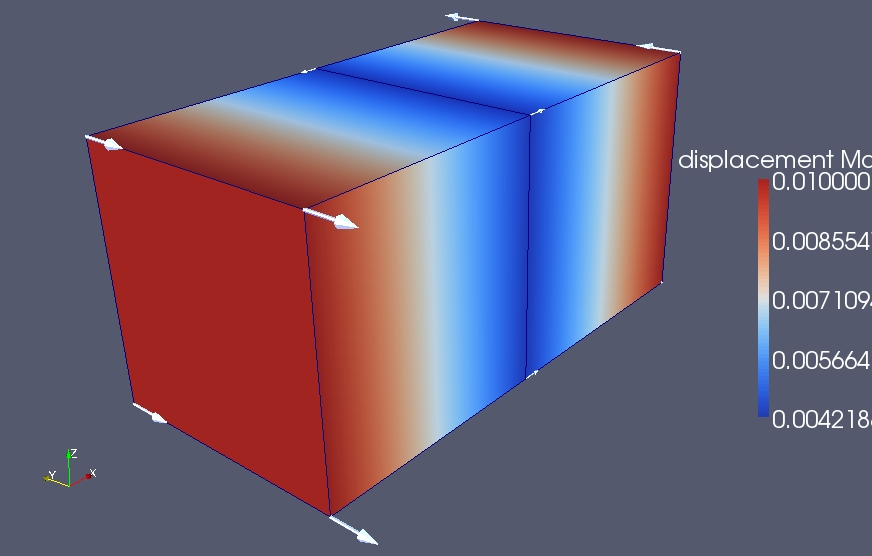
\includegraphics[scale=0.33]{examples/figs/twohex8-sheardisp}
  \caption{Color contours and vectors of displacement for the shear displacement
    example using a mesh composed of two trilinear hexahedral cells.}
  \label{fig:twohex8-shear}
\end{figure}


\subsection{Kinematic Fault Slip Example}

The next example problem is left-lateral fault slip applied between
the two hexahedral cells using kinematic cohesive cells. The vertices
away from the fault are held fixed in the x, y, and z directions.
Parameter settings that override or augment those in \filename{pylithapp.cfg}
are contained in the file \filename{dislocation.cfg}. These settings
include:
\begin{inventory}
  \facilityitem{pylithapp.timedependent.bc.x\_neg}{Defines which degrees of freedom
    are being constrained (x, y, and z), gives the label (\facility{x\_neg},
    defined in \filename{twohex8.mesh}) defining the points desired, and
    assigns a label to the boundary condition set. In this case, we use
    the default spatial database (ZeroDispDB) for the Dirichlet boundary
    condition, which sets the displacements to zero.}
  \facilityitem{pylithapp.timedependent.bc.x\_pos}{Defines which degrees of freedom
    are being constrained (x, y, and z), gives the label (\facility{x\_pos},
    defined in \filename{twohex8.mesh}) defining the points desired, and
    assigns a label to the boundary condition set.}
  \facilityitem{pylithapp.timedependent.interfaces}{Gives the label (defined in
    \filename{twohex8.mesh}) defining the points on the fault, provides
    quadrature information, and then gives database names for material
    properties (needed for conditioning), fault slip, peak fault slip
    rate, and fault slip time.}
\end{inventory}
The fault example requires three additional database files that were
not needed for the simple displacement examples. The first file
(\filename{dislocation\_slip.spatialdb}) specifies 0.01 m of
left-lateral fault slip for the entire fault.  The data dimension is
zero since the same data are applied to all points in the set. The
default slip time function is a step-function, so we also must provide
the time at which slip begins. The elastic solution is associated with
advancing from $t=-dt$ to $t=0$, so we set the slip initiation time
for the step-function to 0 in
\filename{dislocation\_sliptime.spatialdb}.  The files containing
common information (\filename{twohex8.mesh}, \filename{pylithapp.cfg})
along with the problem-specific files (\filename{dislocation.cfg},
\filename{dislocation\_slip.spatialdb},
\filename{dislocation\_sliptime.spatialdb}) provide a complete
description of the problem, and we can then run this example by typing
\begin{shell}
$$ pylith dislocation.cfg
\end{shell}
If the problem ran correctly, you should be able to generate a figure
such as Figure \vref{fig:twohex8-disloc}, which was generated using
ParaView.

\begin{figure}
  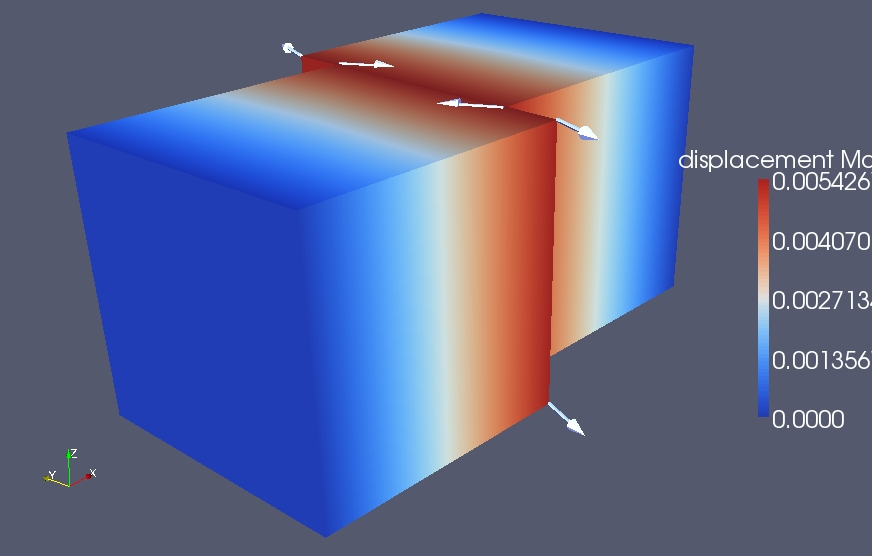
\includegraphics[scale=0.33]{examples/figs/twohex8-dislocation}
  \caption{Color contours and vectors of displacement for the kinematic fault
    example using a mesh composed of two trilinear hexahedral cells.}
  \label{fig:twohex8-disloc}
\end{figure}


% End of file

\section{\label{sec:examples:twotet4-geoproj}Tutorial Using Two Tetrahedra
with Geovreferenced Coordinate System Mesh}

PyLith features discussed in this tutorial:
\begin{itemize}
\item Quasi-static solution
\item Mesh ASCII format
\item Dirichlet boundary conditions
\item Kinematic fault interface conditions
\item Linearly elastic isotropic material
\item VTK output
\item Linear tetrahedral cells
\item SimpleDB spatial database with geographic coordinates
\item SCEC CVM-H spatial database
\item ZeroDispDB spatial database
\end{itemize}
All of the files necessary to run the examples are contained in the
directory \texttt{examples/twocells/twotet4-geoproj.}


\subsection{Overview}

This tutorial is virtually identical to the other tutorial using two
linear tetrahedra (See Section \vref{sec:Tutorial-Two-tet4}). The
primary difference is in how the material properties are assigned.
For this tutorial, the physical properties come from the SCEC CVM-H
database (described in Section \vref{sec:SCEC:CVM-H}). Using the
SCEC CVM-H database is straightforward, requiring only a few modifications
to \texttt{pylithapp.cfg}. Because the SCEC CVM-H database uses geographic
coordinates, we must also use geographic coordinates in the PyLith
mesh ASCII file and other spatial databases. Note that all of these
geographic coordinate systems do not need to be the same. PyLith will
automatically transform from one geographic coordinate system to another
using the spatialdata package. The spatial databases should all use
a geovreferenced Cartesian coordinate system, such as a geographic
projection to insure interpolation is performed properly. Since all
aspects of this problem other than the material database and the coordinate
system are identical to the examples in Section \vref{sec:Tutorial-Two-tet4},
we only describe the kinematic fault problem in this tutorial.


\subsection{Mesh Description}

The mesh consists of two tetrahedra forming a pyramid shape (Figure
\vref{fig:twotet4-geoproj-mesh}). The mesh geometry and topology are
described in the file \texttt{twotet4.mesh}, which is in PyLith mesh
ASCII format. If you compare this mesh against the one used in \vref{sec:Tutorial-Two-tet4},
you will notice that, although the mesh topology is the same, the
vertex coordinates are significantly different. We use zone 11 UTM
coordinates with the NAD27 datum for the mesh. Although we used the
same coordinate system as the SCEC CVM-H, we could have also used
any other geographic projection supported by spatialdata and Proj.4.
See Appendix \vref{sec:spatialdata:SimpleIOAscii} for other examples
of using geographic coordinates. 

\noindent \begin{center}
\begin{figure}
\begin{centering}
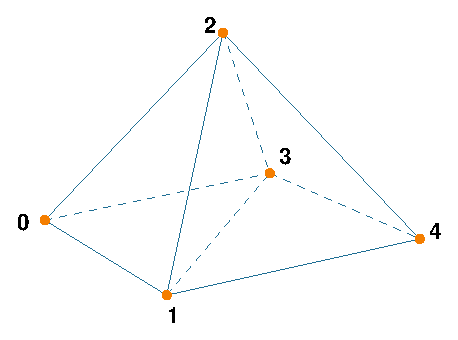
\includegraphics{tutorials/twocells/figs/twotet4-mesh}
\par\end{centering}

\caption{Mesh composed of two linear tetrahedral cells in a geovreferenced coordinate
system used for the example problems.\label{fig:twotet4-geoproj-mesh}}
\end{figure}

\par\end{center}


\subsection{Additional Common Information}

This problem has some unique aspects compared to the other tutorials.
First, all of the other tutorials use a Cartesian coordinate system,
while this one uses a geographic coordinate system. In addition to
using different vertex coordinates, we also define the coordinate
system for the mesh in \texttt{pylithapp.cfg}:
\begin{lyxcode}
{[}pylithapp.mesh\_generator.importer{]}

coordsys~=~spatialdata.geocoords.CSGeoProj

filename~=~twotet4.mesh

coordsys.space\_dim~=~3

~

{[}pylithapp.mesh\_generator.importer.coordsys{]}

datum\_horiz~=~NAD27

datum\_vert~=~mean~sea~level

ellipsoid~=~clrk66

~

{[}pylithapp.mesh\_generator.importer.coordsys.projector{]}

projection~=~utm

proj-options~=~+zone=11~
\end{lyxcode}
At the top level, we define the type of coordinate system, give the
file describing the mesh, and give the number of spatial dimensions
for the coordinate system. We then provide the horizontal datum and
vertical datum for the coordinate system, along with the ellipsoid
to be used. Finally, we specify a UTM projection, and specify zone
11 as the zone to be used.

In addition to the usual material information, we must specify that
we want to use the \texttt{SCECCVMH} database implementation:
\begin{lyxcode}
{[}pylithapp.timedependent.materials.material{]}

db~=~spatialdata.spatialdb.SCECCVMH

db.data\_dir~=~/home/brad/data/sceccvm-h/vx53/bin
\end{lyxcode}
The first \texttt{db} option defines \texttt{SCECCVMH} as the spatial
database to be used. The next line defines the location of the \texttt{vx53}
data files, and must be changed to the location specified by the user
when the package is installed. The package may be obtained from Harvard's
Structural Geology and Tectonics \url{structure.harvard.edu/cvm-h}.

The final difference with the other examples is in the description
of the spatial databases. They must also use geographic coordinates.
Examining \texttt{dislocation\_slip.spatialdb}, we find:
\begin{lyxcode}
//~We~are~specifying~the~data~in~a~projected~geographic~coordinate~system.

cs-data~=~geo-projected~\{

~~to-meters~=~1.0

~~ellipsoid~=~clrk66

~~datum-horiz~=~NAD27

~~datum-vert~=~mean~sea~level

~~projector~=~projection~\{

~~~~projection~=~utm

~~~~units~=~m

~~~~proj-options~=~+zone=11

~~\}

\}
\end{lyxcode}

\subsection{Kinematic Fault Slip Example}

This example problem is a left-lateral fault slip applied between
the two tetrahedral cells using kinematic cohesive cells. Note that
we vary the amount of fault slip for each vertex with this example,
as described in \texttt{}~\linebreak{}
\texttt{dislocation\_slip.spatialdb}. The vertices away from the fault
are held fixed in the x, y, and z directions. Parameter settings that
override or augment those in \texttt{pylithapp.cfg} are contained
in the file \texttt{dislocation.cfg}.

Recall that we condition problems with the kinematic fault interface
using the material properties. Since the material properties are being
defined using the SCEC CVM-H database, this same database should be
used as the material database for the faults. This also applies to
the AbsorbingDampers boundary condition.

The files containing common information (\texttt{twotet4.mesh}, \texttt{pylithapp.cfg})
along with the problem-specific files (\texttt{dislocation.cfg, dislocation\_slip.spatialdb,
dislocation\_sliptime.spatialdb}) provide a complete description of
the problem, and we can then run this example by typing
\begin{lyxcode}
pylith~dislocation.cfg
\end{lyxcode}
If the problem ran correctly, you should be able to generate a figure
such as Figure \vref{fig:twotet4-geoproj-disloc}, which was generated
using ParaView.

\begin{figure}
\begin{centering}
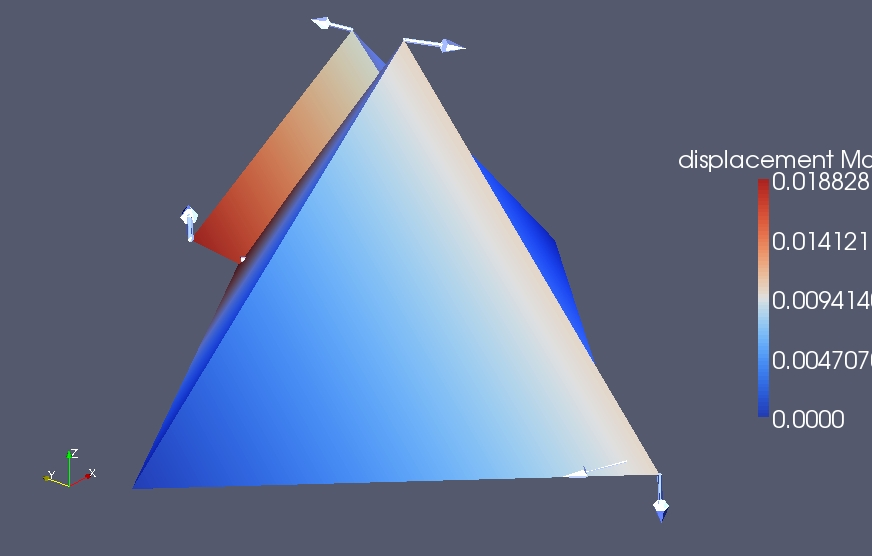
\includegraphics[scale=0.33]{tutorials/twocells/figs/twotet4-geoproj-dislocation}
\par\end{centering}

\caption{Color contours and vectors of displacement for the kinematic fault
example using a mesh composed of two linear tetrahedral cells in a
geovreferenced coordinate system.\label{fig:twotet4-geoproj-disloc}}
\end{figure}

\section{Example Using Tetrahedral Mesh Created by LaGriT}
\label{sec:example:3dtet4}

PyLith features discussed in this example:
\begin{itemize}
\item Quasi-static solution
\item LaGriT mesh format
\item Dirichlet boundary conditions
\item Kinematic fault interface conditions
\item Linearly elastic isotropic material
\item Maxwell linear viscoelastic material
\item Specifying more than one material
\item VTK output
\item Linear tetrahedral cells
\item SimpleDB spatial database
\item ZeroDispDB spatial database
\item Custom algebraic multigrid preconditioner with split fields
\item Global uniform mesh refinement
\end{itemize}
All of the files necessary to run the examples are contained in the
directory \filename{examples/3d/tet4.}


\subsection{Overview}

This example is a simple 3D example of a quasi-static finite element
problem. It is a mesh composed of 852 linear tetrahedra subject to
displacement boundary conditions. This example demonstrates the usage
of the LaGriT mesh generation package \url{lagrit.lanl.gov} to create
a mesh, as well as describing how to use a LaGriT-generated mesh in
PyLith. In this example we will walk through the steps necessary
to construct, run, and visualize the results for two problems that
use the same mesh. For each of these problems we also consider a simulation
using a custom algebraic multigrid preconditioner with a globally
uniformly refined mesh that reduces the node spacing by a factor of
two. In addition to this manual, each of the files for the example
problems includes extensive comments.


\subsection{Mesh Generation and Description}

The mesh for these examples is a simple rectangular prism (Figure
\vref{fig:3dtet4:mesh}). This mesh would be quite difficult to generate
by hand, so we use the LaGriT mesh generation package. For this example,
we provide a documented command file in \filename{examples/3d/tet4.}
Examination of this command file should provide some insight into
how to use LaGriT with PyLith. For more detailed information refer
to the LaGriT website \url{lagrit.lanl.gov}. If you have LaGriT installed
on your machine, you can use the command file to create your own mesh.
Otherwise, you can use the mesh that has already been created.

There are two ways to use the command file. The simplest method is
to go to the \filename{examples/3d/tet4} directory, start LaGriT, and then type:
\begin{shell}
input mesh_tet4_1000m.lagrit
\end{shell}
This will run the commands in that file, which will produce the necessary
files to run the example. This method will create the mesh, but you
will gain very little insight into what is being done. A more informative
approach is to input each command directly. That way, you will see
what each command does. You can simply copy and paste the commands
from \filename{mesh\_tet4\_1000m.lagrit}. For example, the first six
commands, which define the block shape, are
\begin{shell}
define / domain_xm / -3.0e+3
define / domain_xp /  3.0e+3
define / domain_ym / -3.0e+3
define / domain_yp /  3.0e+3
define / domain_zm / -4.0e+3
define / domain_zp /  0.0e+3 
\end{shell}
Continuing through the remainder of the commands in \filename{mesh\_tet4\_1000m.lagrit},
you will eventually end up with the files \filename{tet4\_1000m\_binary.gmv},
\filename{tet4\_1000m\_ascii.gmv}, \filename{tet4\_1000m\_ascii.pset},
and \filename{tet4\_1000m\_binary.pset}. The ASCII files are not actually
needed, but we create them so users can see what is contained in the
files. These files may also be used instead of the binary versions,
if desired. The \filename{.gmv} files define the mesh information, and
they may be read directly by the GMV \url{laws.lanl.gov/XCM/gmv/GMVHome.html}
mesh visualization package. The \filename{.pset} files specify the vertices
corresponding to each set of vertices on a surface used in the problem,
including the fault as well as external boundaries to which boundary
conditions are applied.

\begin{figure}
  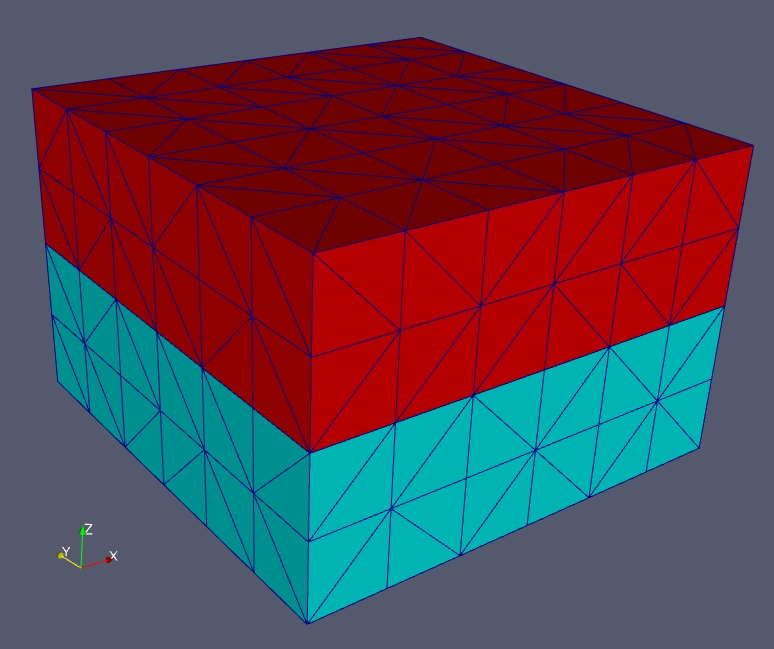
\includegraphics[scale=0.45]{examples/figs/3dtet4_mesh}
  \caption{Mesh composed of linear tetrahedral cells generated by
    LaGriT used for the example problems. The different colors
    represent the different materials.}
  \label{fig:3dtet4:mesh}
\end{figure}


\subsection{Additional Common Information}

In addition to the mesh, the example problems share additional information.
In such cases it is generally useful to create a file named \filename{pylithapp.cfg}
in the run directory, since this file is read automatically every
time PyLith is run. Settings specific to a particular problem may
be placed in other \filename{.cfg} files, as described later, and then
those files are placed on the command line.  The settings contained
in \filename{pylithapp.cfg} for this problem consist of:
\begin{inventory}
  \facilityitem{pylithapp.journal.info}{Settings that control the verbosity of
    the output for the different components.}
  \facilityitem{pylithapp.mesh\_generator}{Settings that control mesh importing,
    such as the importer type, the filenames, and the spatial dimension
    of the mesh.}
  \facilityitem{pylithapp.timedependent}{Settings that control the problem, such
    as the total time, time-step size, and number of entries in the material
    array.}
  \facilityitem{pylithapp.timedependent.materials}{Settings that control the material
    type, specify which material IDs are to be associated with a particular
    material type, and give the name of the spatial database containing
    material parameters for the mesh. The quadrature information is also
    given.}
  \facilityitem{pylithapp.petsc}{PETSc settings to use for the problem, such as
    the preconditioner type.}
\end{inventory}
Since these examples use a mesh from LaGriT, we set the importer to
\object{MeshIOLagrit}:
\begin{cfg}
<h>[pylithapp.mesh_generator]</h>
<f>reader</f> = pylith.meshio.MeshIOLagrit

<h>[pylithapp.mesh_generator.reader]</h>
<p>filename_gmv</p> = mesh/tet4_1000m_binary.gmv
<p>filename_pset</p> = mesh/tet4_1000m_binary.pset
<p>flip_endian</p> = True
# record_header_32bit = False
\end{cfg}
Notice that there are a couple of settings pertinent to binary files.
The first flag (\texttt{flip\_endian}) is used if the binary files
were produced on a machine with a different endianness than the machine
on which they are being read. If you get an error when attempting
to run an example, you may need to change the setting of this flag.
The second flag (\texttt{record\_header\_32bit}) may need to be set
to \texttt{False} if the version of LaGriT being used has 64-bit Fortran
record headers. 

This example differs from previous examples, because we specify two
material groups:
\begin{cfg}
<h>[pylithapp.timedependent]</h>
<f>materials</f> = [elastic, viscoelastic]

<h>[pylithapp.timedependent.materials.elastic]</h>
<p>label</p> = Elastic material
<p>id</p> = 1
<p>db.iohandler.filename</p> = spatialdb/mat_elastic.spatialdb
<f>quadrature.cell</f> = pylith.feassemble.FIATSimplex
<p>quadrature.cell.dimension</p> = 3

<h>[pylithapp.timedependent.materials.viscoelastic]</h>
<p>label</p> = Viscoelastic material
<p>id</p> = 2
<p>db.iohandler.filename</p> = spatialdb/mat_viscoelastic.spatialdb
<f>quadrature.cell</f> = pylith.feassemble.FIATSimplex
<p>quadrature.cell.dimension</p> = 3
\end{cfg}
The two materials correspond to the two different colors in Figure
\vref{fig:3dtet4:mesh}. Each material uses a different spatial database
because the physical parameters are different. In generating the mesh
within LaGriT, the mesh contains four materials as a result of how
LaGriT handles materials and interior interfaces. Near the end of
the LaGriT command file, we merge the materials on each side of the
fault into a single material to simplify the input and output from
PyLith. For this example, values describing three-dimensional elastic
material properties are given by the single point in the spatial databases,
resulting in uniform physical properties within each material.


\subsection{Shear Displacement Example}

The first example problem is shearing of the mesh along the y-direction,
with displacement boundary conditions applied on the planes corresponding
to the minimum and maximum x-values. Parameter settings that override
or augment those in \filename{pylithapp.cfg} are contained in the file
\filename{step01.cfg}. These settings are:
\begin{inventory}
  \facilityitem{pylithapp.timedependent}{Specifies an implicit formulation for
    the problem and specifies the array of boundary conditions.}
  \facilityitem{pylithapp.timedependent.implicit}{Specifies an array of two output
    managers, one for the full domain, and another for a subdomain corresponding
    to the ground surface.}
  \facilityitem{pylithapp.timedependent.bc.x\_pos}{Specifies the boundary conditions
    for the right side of the mesh, defining which degrees of freedom
    are being constrained (\texttt{x} and \texttt{y}), providing the label
    (defined in \filename{tet4\_1000m\_binary.pset}) defining the points
    desired, assigning a label to the boundary condition set, and giving
    the name of the spatial database defining the boundary conditions
    (\filename{fixeddisp\_shear.spatialdb}).}
  \facilityitem{pylithapp.timedependent.bc.x\_neg}{Specifies the boundary conditions
    for the left side of the mesh, defining which degrees of freedom are
    being constrained (\texttt{x} and \texttt{y}), providing the label
    (defined in \filename{tet4\_1000m\_binary.}pset) defining the points
    desired, assigning a label to the boundary condition set, and giving
    the name of the spatial database defining the boundary conditions
    (\filename{fixeddisp\_shear.spatialdb}).}
  \facilityitem{pylithapp.timedependent.bc.z\_neg}{Specifies the boundary conditions
    for the bottom of the mesh, defining which degrees of freedom are
    being constrained (\texttt{x} and \texttt{y}), providing the label
    (defined in \filename{tet4\_1000m\_binary.}pset) defining the points
    desired, assigning a label to the boundary condition set, and giving
    the name of the spatial database defining the boundary conditions
    (\filename{fixeddisp\_shear.spatialdb}).}
  \facilityitem{pylithapp.problem.formulation.output.domain.writer}{Gives the
    base filename for VTK output over the entire domain (\filename{shearxy.vtk}).}
  \facilityitem{pylithapp.problem.formulation.output.subdomain}{Gives the label
    of the nodeset defining the subdomain and gives the base filename
    for VTK output over the subdomain corresponding to the ground surface
    (\filename{step01-groundsurf.vtk}).}
  \facilityitem{pylithapp.timedependent.materials.elastic.output}{Gives the base
    filename for state variable output files for the \texttt{elastic}
    material set (\filename{step01-elastic.vtk}), and causes state variables
    to be averaged over all quadrature points in each cell.}
  \facilityitem{pylithapp.timedependent.materials.viscoelastic.output}{Gives the
    base filename for state variable output files for the \texttt{viscoelastic}
    material set (\filename{step01-viscoelastic.vtk}), and causes state
    variables to be averaged over all quadrature points in each cell.}
\end{inventory}
The values for the Dirichlet boundary conditions are described in
the file \filename{fixeddisp\_shear.spatialdb}, as specified in \filename{step01.cfg}.
The format of all spatial database files is similar. Because data
are being specified using two control points (rather than being uniform
over the mesh, for example), the data dimension is one.

The files containing common information
(\filename{tet4\_1000m\_binary.gmv},
\filename{tet4\_1000m\_binary.pset}, \filename{pylithapp.cfg},
\filename{mat\_elastic.spatialdb}, and
\filename{mat\_viscoelastic.spatialdb}) along with the
problem-specific files (\filename{step01.cfg} and
\filename{fixeddisp\_shear.spatialdb}) provide a complete description
of the problem, and we can then run this example by typing
\begin{shell}
$$ pylith step01.cfg
\end{shell}
Once the problem has run, six files will be produced. The first file
is named \filename{step01\_t0000000.vtk}. The \filename{t0000000}
indicates that the output is for the first (and only) time step,
corresponding to an elastic solution. This file contains mesh
information as well as displacement values at the mesh vertices. The
second file is named
\filename{step01-statevars-elastic\_t0000000.vtk}. This file contains
the state variables for each cell in the material group
\texttt{elastic}.  The default fields are the total strain and stress
fields. These values are computed at each quadrature point in the
cell. We have requested that the values be averaged over all
quadrature points for each cell; however, since we only have a single
quadrature point for each linear tetrahedron, this will have no
effect. The third file
(\filename{step01-statevars-viscoelastic\_info.vtk}) gives the
material properties used for the \texttt{viscoelastic} material
set. Since we have not specified which properties to write, the
default properties (\texttt{mu}, \texttt{lambda}, \texttt{density})
are written.  There are two additional files containing the state
variables for each of the material sets. The final file
(\filename{step01-groundsurf\_t0000000.vtk}) is analogous to
\filename{step01\_t0000000.vtk}, but in this case the results are only
given for a subset of the mesh corresponding to the ground
surface. Also, the cells in this file are one dimension lower than the
cells described in \filename{step01\_t0000000.vtk}, so they are
triangles rather than tetrahedra. All of the \filename{.vtk} files may
be used with a number of visualization packages. If the problem ran
correctly, you should be able to generate a figure such as Figure
\vref{fig:3dtet4:shear}, which was generated using ParaView.

\begin{figure}
  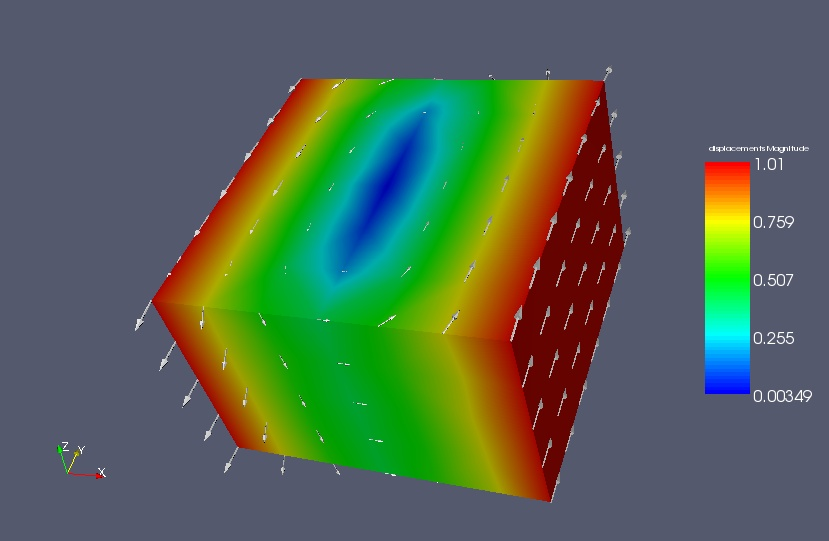
\includegraphics[scale=0.45]{examples/figs/3dtet4_shear}
  \caption{Color contours and vectors of displacement for the axial displacement
    example using a mesh composed of linear tetrahedral cells generated
    by LaGriT.}
  \label{fig:3dtet4:shear}
\end{figure}


\subsubsection{Alternative Solver and Discretization Settings}

Example \filename{step01.cfg} uses the additive Schwarz preconditioner
in conjunction with a classical Gram-Schmidt orthogonalization iterative
solver. This preconditioner works reasonably well but the number of
iterations generally scales with problem size. Even this small, simple
problem requires 24 iterations. In this example (\filename{step02.cfg}),
we use a more sophisticated preconditioner that preconditions the
degrees of freedom associated with the displacement field with an
algebraic multigrid algorithm (see Section \vref{sec:petsc:options}
for details). Additionally, we illustrate the use of global uniform
mesh refinement to increase the resolution of the solution by a factor
of two. Because the mesh is refined in parallel after distribution,
this technique can be used to run a larger problem than would be possible
if the full resolution mesh had to be generated by the mesh generator.
LaGriT runs only in serial and CUBIT has extremely limited parallel
mesh generation capabilities. Table \vref{tab:3dtet4:solver:cmp} shows
the improved efficiency of the solver using the split fields with
the algebraic multigrid preconditioner, especially as the problem
size becomes larger. We have found similar results for other problems.

\begin{table}[htbp]
  \caption{Number of iterations in linear solve for the Shear
    Displacement and Kinematic Fault Slip problems discussed in this
    section. The preconditioner using split fields and an algebraic
    multigrid algorithm solves the linear system with fewer iterations
    with only a small to moderate increase as the problem size grows.}
\label{tab:3dtet4:solver:cmp}
\begin{tabular}{lp{2.0in}ccc}
\textbf{Problem} & \textbf{Preconditioner} & \textbf{Refinement} & \textbf{\# DOF} & \textbf{\# Solve Iterations}\\
\hline 
Shear Displacement & additive Schwarz & none & 546 & 24 (step01) \\
 &  & 2x  & 3890 & 47 \\
 & split fields with algebraic multigrid & none & 546 & 13 \\
 &  & 2x  & 3890 & 28 (step02)\\
Kinematic Fault Slip & additive Schwarz & none & 735 & 28 (step03) \\
 &  & 2x  & 4527 & 63\\
 & split fields with algebraic multigrid & none & 735 & 28 \\
 &  & 2x  & 4527 & 38 (step04) \\
\hline 
\end{tabular}
\end{table}

The field splitting and algebraic multigrid preconditioning are set
up in \filename{step02.cfg} with the following parameters:
\begin{cfg}
<h>[pylithapp.timedependent.formulation]</h>
<p>matrix_type</p> = aij

<h>[pylithapp.petsc]</h>
<p>pc_type</p> = ml
\end{cfg}
The uniform global refinement requires changing just a single parameter:
\begin{cfg}
<h>[pylithapp.mesh_generator]</h>
<f>refiner</f> = pylith.topology.RefineUniform
\end{cfg}

\subsection{Kinematic Fault Slip Example}

The next example problem is a right-lateral fault slip applied on
the vertical fault defined by \texttt{x = 0}. The left and right sides
of the mesh are fixed in the \texttt{x}, \texttt{y}, and \texttt{z}
directions. Parameter settings that override or augment those in \filename{pylithapp.cfg}
are contained in the file \filename{step03.cfg}. These settings are:
\begin{inventory}
  \facilityitem{pylithapp.timedependent}{Specifies an implicit formulation for
    the problem, the array of boundary conditions, and the array of interfaces.}
  \facilityitem{pylithapp.timedependent.implicit}{Specifies an array of two output
    managers, one for the full domain, and another for a subdomain corresponding
    to the ground surface.}
  \facilityitem{pylithapp.timedependent.bc.x\_pos}{Specifies the boundary conditions
    for the right side of the mesh, defining which degrees of freedom
    are being constrained (\texttt{x}, \texttt{y}, and \texttt{z}), providing
    the label (defined in \filename{tet4\_1000m\_binary.pset}) defining
    the points desired, and assigning a label to the boundary condition
    set. Rather than specifying a spatial database file to define the
    boundary conditions, we use the default spatial database (ZeroDispDB)
    for the Dirichlet boundary condition, which sets the displacements
    to zero.}
  \facilityitem{pylithapp.timedependent.bc.x\_neg}{Specifies the boundary conditions
    for the left side of the mesh, defining which degrees of freedom are
    being constrained (\texttt{x}, \texttt{y}, and \texttt{z}), providing
    the label (defined in \filename{tet4\_1000m\_binary.pset}) defining
    the points desired, and assigning a label to the boundary condition
    set. Rather than specifying a spatial database file to define the
    boundary conditions, we use the default spatial database (ZeroDispDB)
    for the Dirichlet boundary condition, which sets the displacements
    to zero.}
  \facilityitem{pylithapp.timedependent.interfaces}{Gives the label (defined in
    \filename{tet4\_1000m\_binary.pset}) defining the points on the fault,
    provides quadrature information, and then gives database names for
    material properties (needed for conditioning), fault slip, peak fault
    slip rate, and fault slip time.}
  \facilityitem{pylithapp.problem.formulation.output.output.writer}{Gives the
    base filename for VTK output over the entire domain (\filename{step03.vtk}).}
  \facilityitem{pylithapp.problem.formulation.output.subdomain}{Gives the label
    of the nodeset defining the subdomain and gives the base filename
    for VTK output over the subdomain corresponding to the ground surface
    (\filename{step03-groundsurf.vtk}).}
  \facilityitem{pylithapp.timedependent.interfaces.fault.output.writer}{Gives
    the base filename for cohesive cell output files 
    (\filename{step03-fault.vtk}).}
  \facilityitem{pylithapp.timedependent.materials.elastic.output}{Gives the base
    filename for state variable output files for the \texttt{elastic}
    material set (\filename{step03-statevars-elastic.vtk}), and causes state
    variables to be averaged over all quadrature points in each cell.}
  \facilityitem{pylithapp.timedependent.materials.viscoelastic.output}{Gives the
    base filename for state variable output files for the \texttt{viscoelastic}
    material set (\filename{step03-statevars-viscoelastic.vtk}), and causes
    state variables to be averaged over all quadrature points in each
    cell.}
\end{inventory}
The fault example requires three additional database files that were
not needed for the simple displacement example. The first file
(\filename{finalslip.spatialdb}) specifies a constant value of 2 m of
right-lateral fault slip that then tapers linearly to zero from 2 km
to 4 km depth, and a linearly-varying amount of reverse slip, with a
maximum of 0.25 m at the surface, linearly tapering to 0 m at 2 km
depth. The data dimension is one since the data vary linearly along a
vertical line. The default slip time function is a step-function, so
we also must provide the time at which slip begins. The elastic
solution is associated with advancing from $t=-dt$ to $t=0$, so we set
the slip initiation time for the step-function to 0 in
\filename{dislocation\_sliptime.spatialdb}.

The files containing common information
(\filename{tet4\_1000m\_binary.gmv},
\filename{tet4\_1000m\_binary.pset}, \filename{pylithapp.cfg},
\filename{mat\_elastic.spatialdb}, and
\filename{mat\_viscoelastic.spatialdb}) along with the
problem-specific files (\filename{step03.cfg},
\filename{finalslip.spatialdb}, and \filename{sliptime.spatialdb})
provide a complete description of the problem, and we can then run
this example by typing
\begin{shell}
$$ pylith step03.cfg
\end{shell}
Once the problem has run, eight files will be produced. The first file
is named \filename{step03\_t0000000.vtk}. The \filename{t0000000}
indicates that the output is for the first (and only) time step,
corresponding to an elastic solution. This file contains mesh
information as well as displacement values at the mesh vertices. The
second file is named
\filename{step03-statevars-elastic\_t0000000.vtk}. This file contains
the state variables for each cell in the material group
\texttt{elastic}.  The default fields are the total strain and stress
fields. We have requested that the values be averaged over all
quadrature points for each cell; however, since we only have a single
quadrature point for each linear tetrahedron, this will have no
effect. The third file
(\filename{step03-statevars-viscoelastic\_info.vtk}) gives the
material properties used for the \texttt{viscoelastic} material
set. Since we have not specified which properties to write, the
default properties (\texttt{mu}, \texttt{lambda}, \texttt{density})
are written. There are two additional files containing the state
variables for each of the material sets. The file
\filename{step03-groundsurf\_t0000000.vtk} is analogous to
\filename{step03\_t0000000.vtk}, but in this case the results are only
given for a subset of the mesh corresponding to the ground
surface. Also, the cells in this file are one dimension lower than the
cells described in \filename{step03\_t0000000.vtk}, so they are
triangles rather than tetrahedra. The file
\filename{step03-fault\_t0000000.vtk} gives the specified fault slip
for each vertex on the fault, along with the computed traction change
for the cohesive cell. The final file,
\filename{step03-fault\_info.vtk}, provides information such as the
normal direction, final slip, and slip time for each vertex on the
fault. All of the \filename{.vtk} files may be used with a number of
visualization packages. If the problem ran correctly, you should be
able to generate a figure such as Figure\vref{fig:3dtet:dislocation},
which was generated using ParaView.

\begin{figure}
  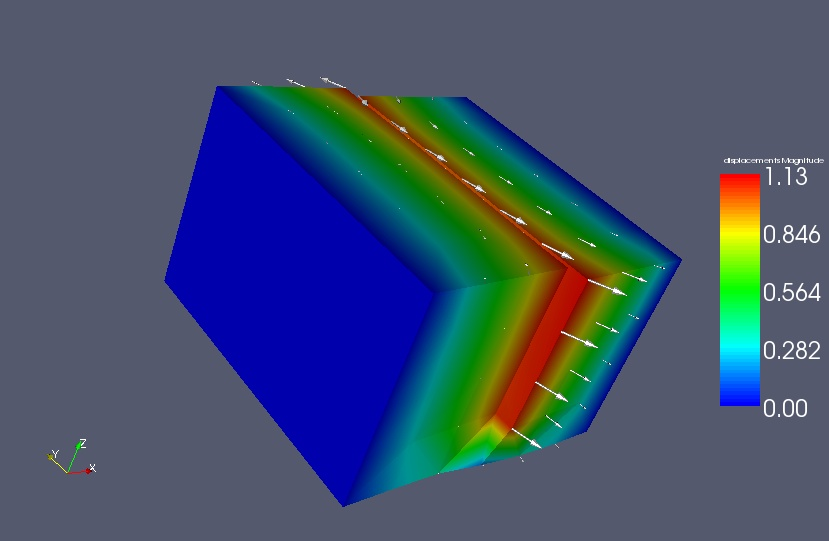
\includegraphics[scale=0.45]{examples/figs/3dtet4_dislocation}
  \caption{Color contours and vectors of displacement for the
    kinematic fault example using a mesh composed of linear
    tetrahedral cells generated by LaGriT.}
  \label{fig:3dtet:dislocation}
\end{figure}


\subsubsection{Alternative Solver and Discretization Settings}

As we did for the Shear Dislocation examples, in \filename{step04.cfg}
we switch to using the split fields and algebraic multigrid preconditioner
along with global uniform mesh refinement. Because PyLith implements
fault slip using Lagrange multipliers, we make a few small adjusments
to the solver settings. As discussed in Section \vref{sec:petsc:options},
we use a custom preconditioner for the Lagrange multiplier degrees
of freedom when preconditioning with field splitting. Within \filename{step04.cfg}
we turn on the use of the custom preconditioner for the Lagrange multiplier
degrees of freedom and add the corresponding settings for the fourth
field for the algebraic multigrid algorithm,
\begin{cfg}
<h>[pylithapp.timedependent.formulation]</h>
<p>split_fields</p> = True
<p>use_custom_constraint_pc</p> = True
<p>matrix_type</p> = aij

<h>[pylithapp.petsc]</h>
<p>fs_pc_type</p> = fieldsplit
<p>fs_pc_use_amat</p> = true
<p>fs_pc_fieldsplit_type</p> = multiplicative
<p>fs_fieldsplit_displacement_pc_type</p> = ml
<p>fs_fieldsplit_lagrange_multiplier_pc_type</p> = jacobi
<p>fs_fieldsplit_displacement_ksp_type</p> = preonly
<p>fs_fieldsplit_lagrange_multiplier_ksp_type</p> = preonly
\end{cfg}
Table \vref{tab:3dtet4:solver:cmp} shows the improved efficiency of
the solver using the split fields with the algebraic multigrid preconditioner.


% End of file
\section{Examples Using Hexahedral Mesh Created by CUBIT/Trelis}
\label{sec:example:3dhex8}

PyLith features discussed in this set of examples:
\begin{itemize}
\item Static solution
\item Quasi-static solution
\item CUBIT/Trelis mesh format
\item Trilinear hexahedral cells
\item VTK output
\item HDF5 output
\item Dirichlet displacement and velocity boundary conditions
\item Neumann traction boundary conditions and time-varying tractions
\item ZeroDispDB spatial database
\item SimpleDB spatial database
\item UniformDB spatial database
\item Static fault rupture
\item Multiple kinematic fault ruptures
\item Specifying more than one material
\item Nonlinear solver
\item Linearly elastic isotropic material
\item Maxwell linear viscoelastic material
\item Generalized Maxwell linear viscoelastic material
\item Power-law viscoelastic material
\item Drucker-Prager elastoplastic material
\item Adaptive time stepping
\item Static fault friction
\item Slip-weakening fault friction
\item Rate-and-state fault friction
\item Gravitational body forces
\item Initial stresses
\item Finite strain
\end{itemize}
All of the files necessary to run the examples are contained in the
directory \filename{examples/3d/hex8}.


\subsection{Overview}

This example is meant to demonstrate most of the important features of
PyLith as a quasi-static finite-element code, using a sequence of
example problems. All problems use the same 3D hexahedral mesh
generated using CUBIT/Trelis (CUBIT is available to employees of the
United States government through \url{cubit.sandia.gov} and Trelis
licenses are available through \url{www.csimsoft.com/trelis}). Each
example builds on the previous examples, as we demonstrate new
features. As in the other examples, the files include extensive
comments. We start with the generation of the mesh, which is composed
of 144 hexahedra. Following the
discussion of how to generate the mesh, we discuss the
\filename{pylithapp.cfg} file, which contains information common to
all the simulations. We group the examples into four sections, each
pertaining to a particular set of PyLith features. We suggest users go
through each of these sections in order as the complexity increases at
each step.


\subsection{Mesh Generation and Description}

The mesh for these examples is a simple rectangular solid (Figure
\vref{fig:3dhex8:mesh}). Although it would be possible to generate
this mesh by hand, we use this example to illustrate the use of
CUBIT/Trelis for mesh generation. We provide documented journal files
in \filename{examples/3d/hex8/mesh.} Dissection of these journal files
should provide some insight into how to use CUBIT/Trelis with
PyLith. For more detailed information on using CUBIT/Trelis, refer to
the CUBIT/Trelis documentation. If you have CUBIT/Trelis installed on
your machine, you can use the journal files to create your own
mesh. Otherwise, you can use the mesh that has already been created.

If you are using CUBIT/Trelis to generate your own mesh, there are two
ways to use the journal files. The simplest method is to go to the
\textsf{Tools} menu, select \textsf{Play Journal File}, and then
select the file \filename{mesh\_hex8\_1000m.jou}. This will run the
commands in that file as well as the commands in
\filename{geometry.jou}, which is referenced from
\filename{mesh\_hex8\_1000m.jou}. Prior to doing this, you should set
your directory to the one containing the journal files. This method
will create the mesh, but you will gain very little insight into what
is being done. A more informative approach is to input each journal
command into the CUBIT command window directly.  That way, you will
see what each command does. The first command in
\filename{mesh\_hex8\_1000m.jou} is \textsf{playback geometry.jou}, so
you should start with the commands in \filename{geometry.jou}. The
first three commands, which define the block shape, are
\begin{shell}
reset
brick x 6000 y 6000 z 4000
volume 1 move x 0 y 0 z -2000
\end{shell}
Continuing through the remainder of the commands in \filename{geometry.jou},
and then using the additional commands in \filename{mesh\_hex8\_1000m.jou},
you will eventually end up with the file \filename{box\_hex8\_1000m.exo},
which contains all of the mesh information. This information is similar
to that included in PyLith mesh ASCII format, but the information
is contained in an Exodus file, which is a specialized netCDF file.
If you have the \filename{ncdump} command available, you can see what
is in the file by typing:
\begin{shell}
$$ ncdump box_hex8_1000m.exo
\end{shell}

\begin{figure}
  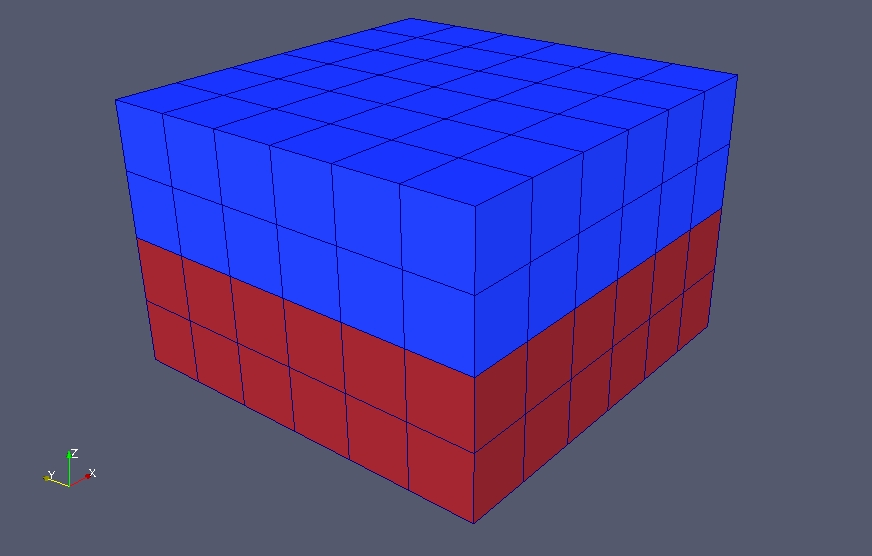
\includegraphics[scale=0.33]{examples/figs/3dhex8_mesh}
  \caption{Mesh composed of trilinear hexahedral cells generated by CUBIT used
    for the suite of example problems. The different colors represent
    the two different materials.}
  \label{fig:3dhex8:mesh}
\end{figure}


\subsection{Additional Common Information}

In addition to the mesh, the example problems share other information.
As in previous examples, we place this information in \filename{pylithapp.cfg}.
Since these examples use a mesh from CUBIT, in this file we set the
importer to \object{MeshIOCubit}:
\begin{cfg}
<h>[pylithapp.mesh_generator]</h>
<f>reader</f> = pylith.meshio.MeshIOCubit

<h>[pylithapp.mesh_generator.reader]</h>
<p>filename</p> = mesh/box_hex8_1000m.exo
\end{cfg}
This example differs from some earlier examples, because we specify
two material groups:
\begin{cfg}
<h>[pylithapp.timedependent]</h>
<f>materials</f> = [upper_crust, lower_crust]</h>

<h>[pylithapp.timedependent.materials.upper_crust]</h>
<p>label</p> = Upper crust material
<p>id</p> = 1
<p>db.iohandler.filename</p> = spatialdb/mat_elastic.spatialdb
<f>quadrature.cell</f> = pylith.feassemble.FIATLagrange
<p>quadrature.cell.dimension</p> = 3

<h>[pylithapp.timedependent.materials.lower_crust]</h>
<p>label</p> = Lower crust material
<p>id</p> = 2
<p>db.iohandler.filename</p> = spatialdb/mat\_elastic.spatialdb
<f>quadrature.cell</f> = pylith.feassemble.FIATLagrange
<p>quadrature.cell.dimension</p> = 3
\end{cfg}
The two material groups correspond to the two different colored regions
in Figure \vref{fig:3dhex8:mesh}. Using two material groups allows
us to specify different material types or material variations for
the upper crust and lower crust, if desired. For now, we retain the
default \object{ElasticIsotropic3D} material type for both materials.
This behavior will be overridden by example-specific\filename{.cfg}
files in some of the examples. Although the material groups are specified
in \filename{pylithapp.cfg}, the physical properties for the material
models are given in \filename{spatialdb/} 
\filename{mat\_elastic.spatialdb}. This spatial database provides values
at a single point, resulting in uniform properties within the material.


\subsection{Example Problems}

The example problems are divided into categories that roughly correspond
to simple static problems, quasi-static problems, problems involving
fault friction, and problems where gravity is used. For the most part,
each successive example involves just adding or changing a few parameters
from the previous example. For this reason, it is advisable to go
through each example in order, starting with the simplest (static
problems).

\subsection{Static Examples}
\label{sec:example:3dhex8-static}

PyLith features discussed in this example:
\begin{itemize}
\item Static solution
\item VTK output
\item Dirichlet displacement boundary conditions
\item Neumann traction boundary conditions
\item ZeroDispDB spatial database
\item SimpleDB spatial database
\item UniformDB spatial database
\item Static fault rupture
\item Specifying more than one material
\item Linearly elastic isotropic material
\end{itemize}

\subsubsection{Overview}

This set of examples describe the simplest class of problems for PyLith.
The problems are all purely elastic, and there is no time-dependence.
This set of elastostatic examples primarily demonstrates the application
of different types of boundary conditions in PyLith, as well as demonstrating
the use of a kinematic fault for a static problem. All of the examples
are contained in the directory \filename{examples/3d/hex8}, and the
corresponding \filename{.cfg} files are \filename{step01.cfg}, \filename{step02.cfg},
and \filename{step03.cfg}. Each example may be run as follows:
\begin{shell}
$ pylith stepXX.cfg
\end{shell}
This will cause PyLith to read the default parameters in \filename{pylithapp.cfg},
and then override or augment them with the additional parameters in
the \filename{stepXX.cfg} file. Each \filename{.cfg} file is extensively
documented to provide detailed information on the various parameters.


\subsubsection{Step01 - Pure Dirichlet Boundary Conditions}

The \filename{step01.cfg} file defines a problem with pure Dirichlet
(displacement) boundary conditions corresponding to compression in the
x-direction and shear in the y-direction. The bottom (minimum z)
boundary is held fixed in the z-direction. On the positive and
negative x-faces, compressional displacements of 1 m are applied in
the x-direction and shear displacements yielding a left-lateral sense
of shear are applied in the y-direction. In this example and in
subsequent examples we would like to output the displacement solution
over a subset of the domain corresponding to the ground surface.

\begin{cfg}
<h>[pylithapp.timedependent.implicit]</h>
# Set the output to an array of 2 output managers.
# We will output the solution over the domain and the ground surface.
<f>output</f> = [domain,subdomain]

# Set subdomain component to OutputSolnSubset (boundary of the domain).
<f>output.subdomain</f> = pylith.meshio.OutputSolnSubset

# Give basename for VTK domain output of solution over ground surface.
<h>[pylithapp.problem.formulation.output.subdomain]</h>
# Name of nodeset for ground surface.
<p>label</p> = face_zpos
<p>writer.filename</p> = output/step01-groundsurf.vtk
\end{cfg}
For the boundary conditions, we must describe which degrees of freedom
are being constrained (\facility{bc\_dof}), we must provide a the label
associated with the CUBIT/Trelis nodeset associated with the BC, and we must
specify the type of spatial database is being used to describe the
boundary conditions. For the x-faces, we use a \object{SimpleDB} to
provide the displacements on the x-faces:
\begin{cfg}
# Boundary condition on +x face
<h>[pylithapp.timedependent.bc.x_pos]</h>
<p>bc_dof</p> = [0, 1]
<p>label</p> = face_xpos
<f>db_initial</f> = spatialdata.spatialdb.SimpleDB
<p>db_initial.label</p> = Dirichlet BC on +x
<p>db_initial.iohandler.filename</p> = spatialdb/fixeddisp_axial_shear.spatialdb

# Boundary condition on -x face
<h>[pylithapp.timedependent.bc.x_neg]</h>
<p>bc_dof</p> = [0, 1]
<p>label</p> = face_xneg
<f>db_initial</f> = spatialdata.spatialdb.SimpleDB
<p>db_initial.label</p> = Dirichlet BC on -x
<p>db_initial.iohandler.filename</p> = spatialdb/fixeddisp_axial_shear.spatialdb
\end{cfg}
For a \object{SimpleDB}, we must provide a filename. The default spatial
database for \facility{db\_initial} is \object{ZeroDispBC}, which automatically
applies zero displacements to all vertices in the nodeset, and no
filename is required (or needed).
\begin{cfg}
# Boundary condition on -z face
<h>[pylithapp.timedependent.bc.z_neg]</h>
<p>bc_dof</p> = [2]
<p>label</p> = face_zneg
<p>db_initial.label</p> = Dirichlet BC on -z
\end{cfg}
When we have run the simulation, the output VTK files will be contained
in \filename{examples/3d/hex8/output} (all with a prefix of \filename{step01}).
Results using ParaView are shown in Figure \vref{fig:example:3dhex8:step01:displacement}.

\begin{figure}
  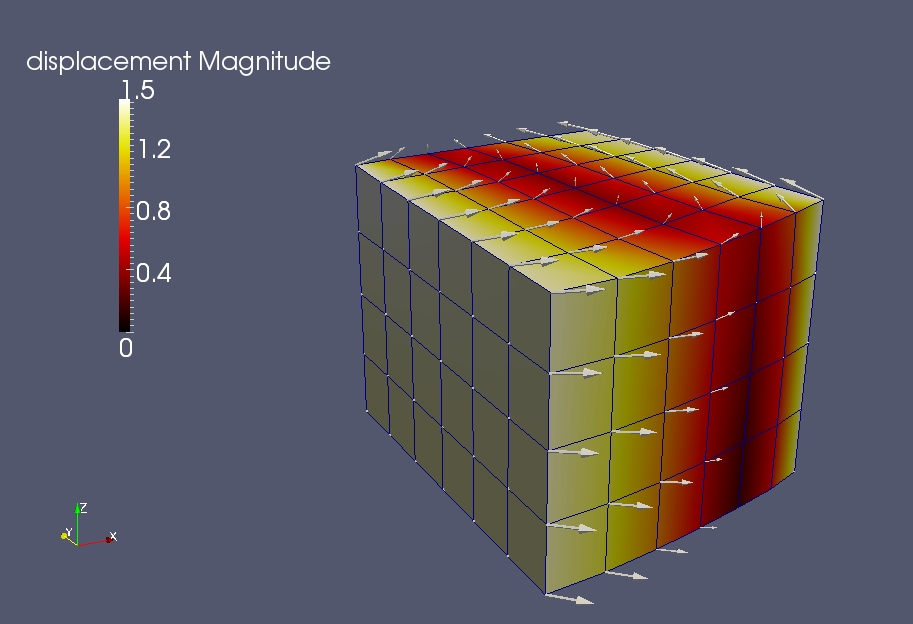
\includegraphics[width=10cm]{examples/figs/3dhex8_step01-displ}
  \caption{Displacement field for example step01 visualized using ParaView. The
    mesh has been distorted by the computed displacements (magnified by
    500), and the vectors show the computed displacements.}
  \label{fig:example:3dhex8:step01:displacement}
\end{figure}


\subsubsection{Step02 - Dirichlet and Neumann Boundary Conditions}

The \filename{step02.cfg} file defines a problem with Dirichlet (displacement)
boundary conditions corresponding to zero x and y-displacements applied
on the negative x-face and Neumann (traction) boundary conditions
corresponding to normal compression and horizontal shear applied on
the positive x-face. The bottom (negative z) boundary is held fixed
in the z-direction. The problem is similar to example step01, except
that 1 MPa of normal compression and 1 MPa of shear (in a left-lateral
sense) are applied on the positive x-face, and the negative x-face
is pinned in both the x and y-directions.

For the boundary conditions, we must first change the boundary condition
type for the positive x-face from the default Dirichlet to Neumann:
\begin{cfg}
# +x face -- first change bc type to Neumann
<h>[pylithapp.timedependent.bc]</h>
<f>x_pos</f> = pylith.bc.Neumann 
\end{cfg}
We use a \object{SimpleDB} to describe the traction boundary
conditions.  When applying traction boundary conditions over a
surface, it is also necessary to specify integration information for
the surface. Since this is a three-dimensional problem, the dimension
of the surface is 2. Since the cells being used are trilinear
hexahedra, the cell type is \object{FIATLagrange} and we use an
integration order of 2.  A lower integration order would not provide
sufficient accuracy while a higher integration order would offer no
benefit (while requiring more computation time and storage):
\begin{cfg}
# Boundary condition on +x face
<h>[pylithapp.timedependent.bc.x_pos]</h>
<p>label</p> = face_xpos
<f>db_initial</f> = spatialdata.spatialdb.SimpleDB
<p>db_initial.label</p> = Neumann BC on +x
<p>db_initial.iohandler.filename</p> = spatialdb/tractions_axial_shear.spatialdb

# We must specify quadrature information for the cell faces.
<f>quadrature.cell</f> = pylith.feassemble.FIATLagrange
<p>quadrature.cell.dimension</p> = 2
<p>quadrature.cell.quad_order</p> = 2 
\end{cfg}
The boundary conditions on the negative x-face are simpler than they
were in example step01 (zero displacements in the x and y-directions),
so we can use the default \object{ZeroDispBC}:
\begin{cfg}
# Boundary condition on -x face
<h>[pylithapp.timedependent.bc.x_neg]</h>
<p>bc_dof</p> = [0, 1] 
<p>label</p> = face_xneg
<p>db_initial.label</p> = Dirichlet BC on -x 
\end{cfg}
The boundary conditions on the negative z-face are supplied in the
same manner as for example step01. When we have run the simulation,
the output VTK files will be contained in \filename{examples/3d/hex8/output}
(all with a prefix of \filename{step02}). Results using ParaView are
shown in Figure \vref{fig:example:3dhex8:step02:displacement}.

\begin{figure}
  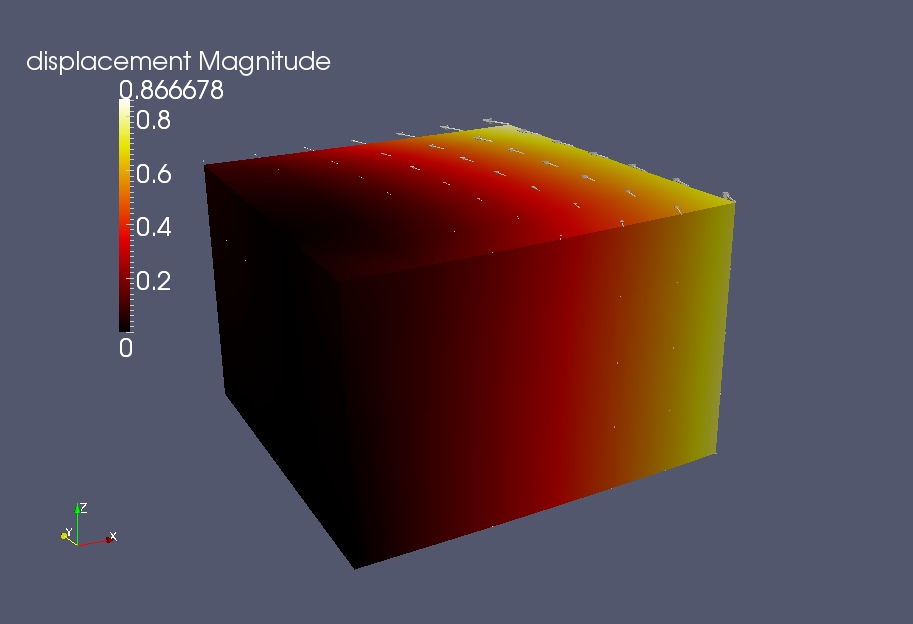
\includegraphics[width=10cm]{examples/figs/3dhex8_step02-displ}
  \caption{Displacement field for example step02 visualized using ParaView. The
    mesh has been distorted by the computed displacements (magnified by
    500), and the vectors show the computed displacements.}
  \label{fig:example:3dhex8:step02:displacement}
\end{figure}


\subsubsection{Step03 - Dirichlet Boundary Conditions with Kinematic Fault Slip}

The \filename{step03.cfg} file describes a problem with Dirichlet (displacement)
boundary conditions corresponding to zero x and y-displacements applied
on the negative and positive x-faces and a vertical fault with a combination
of left-lateral and updip motion. The left-lateral component of fault
slip has a constant value of 2 m in the upper crust, and then decreases
linearly to zero at the base of the model. The reverse slip component
has a value of 0.25 m at the surface, and then decreases linearly
to zero at 2 km depth.

Due to the simplicity of the boundary conditions, we are able to use
the default \object{ZeroDispBC} for the positive and negative x-faces,
as well as the negative z-face. To use a fault, we must first define
a fault interface. We do this by providing an array containing a single
interface. For this example we specify the fault slip, so we set the interface
type to \object{FaultCohesiveKin}.
\begin{cfg}
<h>[pylithapp.timedependent]</h>
# Set interfaces to an array of 1 fault: 'fault'.
<f>interfaces</f> = [fault] 

# Set the type of fault interface condition.
<h>[pylithapp.timedependent.interfaces]</h>
<f>fault</f> = pylith.faults.FaultCohesiveKin 

<h>[pylithapp.timedependent.interfaces.fault]</h>
# The label corresponds to the name of the nodeset in CUBIT/Trelis.
<p>label</p> = fault

# We must define the quadrature information for fault cells.
# The fault cells are 2D (surface).
<f>quadrature.cell</f> = pylith.feassemble.FIATLagrange
<p>quadrature.cell.dimension</p> = 2 
\end{cfg}
We retain the default \object{StepSlipFn} since we want static fault
slip. Finally, we use one \object{SimpleDB} to define the spatial
variation of fault slip, and another \object{SimpleDB} to define the
spatial variation in slip initiation times (the start time is 0.0
everywhere since this is a static problem):
\begin{cfg}
# The slip time and final slip are defined in spatial databases.
<h>[pylithapp.timedependent.interfaces.fault.eq\_srcs.rupture.slip\_function]</h>
<p>slip.iohandler.filename</p> = spatialdb/finalslip.spatialdb
<p>slip.query_type</p> = linear
<p>slip_time.iohandler.filename</p> = spatialdb/sliptime.spatialdb 

# Fault output, give the basename for the VTK file.
<h>[pylithapp.problem.interfaces.fault.output]</h>
<p>writer.filename</p> = output/step03-fault.vtk 
\end{cfg}
This will result in two extra files being produced. The first file
(\filename{step03-fault\_info.vtk}) contains information such as the
normal directions to the fault surface, the applied fault slip, and
the fault slip times. The second file
(\filename{step03-fault\_t0000000.vtk}) contains the cumulative fault
slip for the time step and the change in tractions on the fault
surface due to the slip. When we have run the simulation, the output
VTK files will be contained in \filename{examples/3d/hex8/output} (all
with a prefix of \filename{step03}). Results using ParaView are shown
in Figure \vref{fig:example:3dhex8:step03-displacement}.

\begin{figure}
  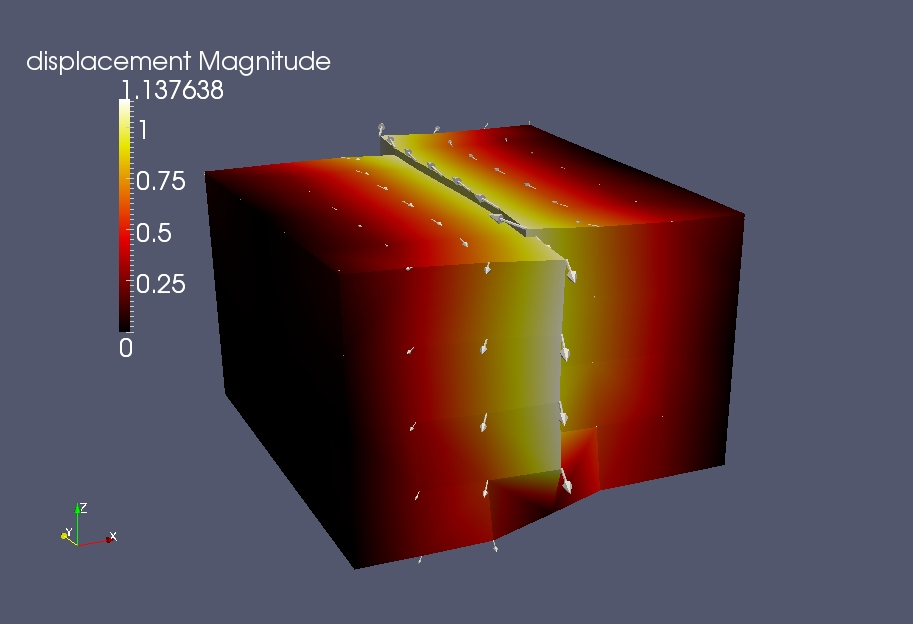
\includegraphics[width=10cm]{examples/figs/3dhex8_step03-displ}
  \caption{Displacement field for example step03 visualized using ParaView. The
    mesh has been distorted by the computed displacements (magnified by
    500), and the vectors show the computed displacements.}
  \label{fig:example:3dhex8:step03-displacement}
\end{figure}


% End of file

\subsection{Quasi-Static Examples}
\label{sec:example:3dhex8-quasistatic}

PyLith features discussed in this example:
\begin{itemize}
\item Quasi-static solution
\item Formatting timestamps of VTK output files
\item HDF5 output
\item Output of velocity field
\item Dirichlet displacement and velocity boundary conditions
\item Neumann traction boundary conditions and time-varying tractions
\item UniformDB spatial database
\item CompositeDB spatial database
\item Quasi-static fault rupture and fault creep
\item Multiple kinematic fault ruptures
\item Specifying more than one material
\item Nonlinear solver
\item Maxwell linear viscoelastic material
\item Power-law viscoelastic material
\item Drucker-Prager elastoplastic material
\item Adaptive time stepping
\end{itemize}

\subsubsection{Overview}

This set of examples describes a set of quasi-static problems for
PyLith. These quasi-static problems primarily demonstrate the usage
of time-dependent boundary conditions and fault slip, as well as different
rheologies. Some of the examples also demonstrate the usage of the
nonlinear solver, which is required by the nonlinear rheologies (power-law
viscoelastic and Drucker-Prager elastoplastic). Some of the examples
also demonstrate the usage of HDF5 output, which is an alternative
to the default VTK output. All of the examples are contained in the
directory \filename{examples/3d/hex8}, and the corresponding \filename{cfg}
files are \filename{step04.cfg}, \filename{step05.cfg}, \filename{step06.cfg},
\filename{step07.cfg}, \filename{step08.cfg}, and \filename{step09.cfg}.
Each example may be run as follows:
\begin{shell}
$ pylith stepXX.cfg
\end{shell}
This will cause PyLith to read the default parameters in \filename{pylithapp.cfg},
and then override or augment them with the additional parameters in
the \filename{stepXX.cfg} file. Each \filename{cfg} file is extensively
documented, to provide detailed information on the various parameters.


\subsubsection{Step04 - Pure Dirichlet Velocity Boundary Conditions}

The \filename{step04.cfg} file defines a problem with x-displacements
fixed at zero on the positive and negative x-faces while velocity
boundary conditions are applied in the y-directions on the same faces,
yielding a left-lateral sense of movement. The bottom (negative z)
boundary is held fixed in the z-direction. We also use a Maxwell viscoelastic
material for the lower crust, and the simulation is run for 200 years
using a constant time-step size of 20 years. The default time stepping
behavior is \object{TimeStepUniform}. We retain that behavior for
this problem and provide the total simulation time and the time-step
size:
\begin{cfg}
# Change the total simulation time to 200 years, and use a constant time
# step size of 20 years.
<h>[pylithapp.timedependent.implicit.time_step]<.h>
<p>total_time</p> = 200.0*year
<p>dt</p> = 20.0*year 
\end{cfg}
We then change the material type of the lower crust, provide a spatial
database from which to obtain the material properties (using the default
\object{SimpleDB}), and request additional output information for
the material:
\begin{cfg}
# Change material type of lower crust to Maxwell viscoelastic.
<h>[pylithapp.timedependent]</h>
<f>materials.lower_crust</f> = pylith.materials.MaxwellIsotropic3D

# Provide a spatial database from which to obtain property values.
# Since there are additional properties and state variables for the Maxwell
# model, we explicitly request that they be output. Properties are named in
# cell_info_fields and state variables are named in cell_data_fields.
<h>[pylithapp.timedependent.materials.lower_crust]</h>
<p>db_properties.iohandler.filename</p> = spatialdb/mat_maxwell.spatialdb
<p>output.cell_info_fields</p> = [density, mu, lambda, maxwell_time]
<p>output.cell_data_fields</p> = [total_strain, stress, viscous_strain]
\end{cfg}
Note that the default \property{output.cell\_info\_fields} are those
corresponding to an elastic material (\texttt{density}, \texttt{mu},
\texttt{lambda}), and the default \property{output.cell\_data\_fields}
are \texttt{total\_strain} and \texttt{stress}. For materials other
than elastic, there are generally additional material properties and
state variables, and the appropriate additional fields must be specifically
requested for each material type.

This example has no displacements in the elastic solution (t = 0),
so we retain the default \object{ZeroDispDB} for all instances of
\facility{db\_initial}. To apply the velocity boundary conditions, we
must specify \facility{db\_rate}, which is zero by default. We use a
\object{UniformDB} to assign the velocities:
\begin{cfg}
# Boundary condition on +x face
<h>[pylithapp.timedependent.bc.x_pos]</h>
<p>bc_dof</p> = [0, 1]
<p>label</p> = face_xpos
<p>db_initial.label</p> = Dirichlet BC on +x
<f>db_rate</f> = spatialdata.spatialdb.UniformDB
<p>db_rate.label</p> = Dirichlet rate BC on +x
<p>db_rate.values</p> = [displacement-rate-x, displacement-rate-y, rate-start-time]
<p>db_rate.data</p> = [0.0*cm/year, 1.0*cm/year, 0.0*year]

# Boundary condition on -x face
<h>[pylithapp.timedependent.bc.x_neg]</h>
<p>bc_dof</p> = [0, 1]
<p>label</p> = face_xneg
<p>db_initial.label</p> = Dirichlet BC on -x
<f>db_rate</f> = spatialdata.spatialdb.UniformDB
<p>db_rate.label</p> = Dirichlet rate BC on +x
<p>db_rate.values</p> = [displacement-rate-x, displacement-rate-y, rate-start-time]
<p>db_rate.data</p> = [0.0*cm/year, -1.0*cm/year, 0.0*year]
\end{cfg}
Note that \facility{db\_rate} requires a start time, which allows the
condition to be applied at any time during the simulation. For this
example, we start the velocity boundary conditions at t = 0.

Finally, we must provide information on VTK output. This is slightly
more complicated than the static case, because we must decide the
frequency with which output occurs for each output manager. We also
assign a more user-friendly format to the output file time stamp,
and we request that the time stamp is in units of 1 year (rather than
the default value of seconds):
\begin{cfg}
# Give basename for VTK domain output of solution over domain.
<h>[pylithapp.problem.formulation.output.domain]</h>
# We specify that output occurs in terms of a given time frequency, and
# ask for output every 40 years. The time stamps of the output files are
# in years (rather than the default of seconds), and we give a format for
# the time stamp.
<p>output_freq</p> = time_step
<p>time_step</p> = 40.0*year
<p>writer.filename</p> = output/step04.vtk
<p>writer.time_format</p> = \%04.0f
<p>writer.time_constant</p> = 1.0*year

# Give basename for VTK domain output of solution over ground surface.
<h>[pylithapp.problem.formulation.output.subdomain]</h>
<p>label</p> = face_zpos ; Name of nodeset for ground surface
# We keep the default output frequency behavior (skip every n steps), and
# ask to skip 0 steps between output, so that we get output every time step.
<p>skip</p> = 0
<p>writer.filename</p> = output/step04-groundsurf.vtk
<p>writer.time_format</p> = %04.0f
<p>writer.time_constant</p> = 1.0*year
\end{cfg}
We provide similar output information for the two materials (\facility{upper\_crust}
and \facility{lower\_crust}). Note that for the domain output, we requested
output in terms of a given time frequency, while for the subdomain
we requested output in terms of number of time steps. When we have
run the simulation, the output VTK files will be contained in \filename{examples/3d/hex8/output}
(all with a prefix of \filename{step04}). Results using ParaView are
shown in Figure \vref{fig:example:3dhex8:step04:displacement}.

\begin{figure}
  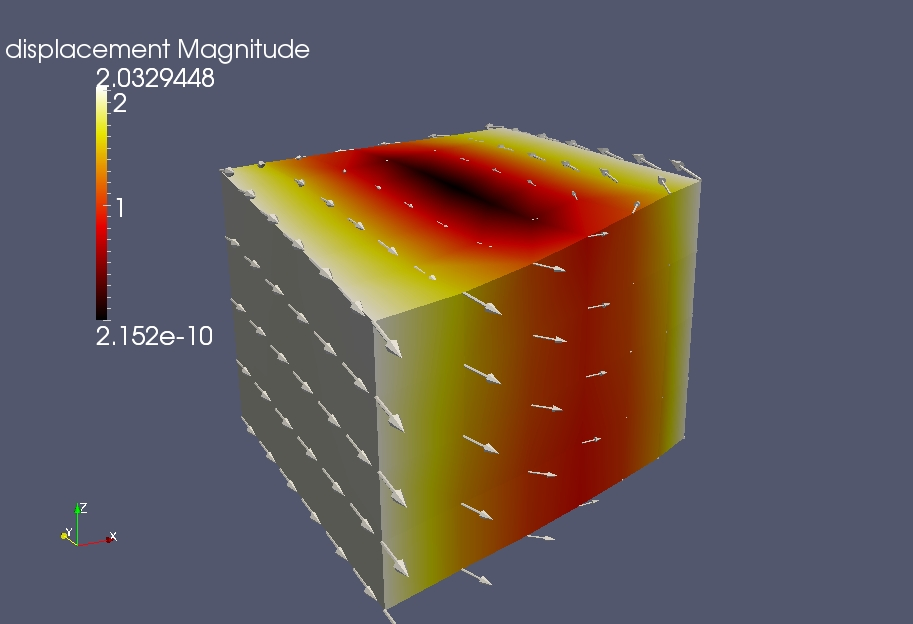
\includegraphics[width=10cm]{examples/figs/3dhex8_step04-displ-t200}
  \caption{Displacement field for example step04 at t = 200 years
    visualized using ParaView. The mesh has been distorted by the
    computed displacements (magnified by 500), and the vectors show
    the computed displacements.}
  \label{fig:example:3dhex8:step04:displacement}
\end{figure}


\subsubsection{Step05 - Time-Varying Dirichlet and Neumann Boundary Conditions}

The \filename{step05.cfg} file describes a problem with time-varying
Dirichlet and Neumann boundary conditions. The example is similar
to example step04, with a few important differences:
\begin{itemize}
\item The Dirichlet boundary conditions on the negative x-face include an
  initial displacement (applied in the elastic solution), as well as
  a constant velocity.
\item Neumann (traction) boundary conditions are applied in the negative
  x-direction on the positive x-face, giving a compressive stress. An
  initial traction is applied in the elastic solution, and then at t
  = 100 years it begins decreasing linearly until it reaches zero at
  the end of the simulation (t = 200 years).
\end{itemize}
We again use a Maxwell viscoelastic material for the lower crust.

For the boundary conditions, we must first change the boundary condition
type for the positive x-face from the default Dirichlet to Neumann:
\begin{cfg}
# +x face -- first change bc type to Neumann
<h>[pylithapp.timedependent.bc]</h>
<f>x_pos</f> = pylith.bc.Neumann 
\end{cfg}
We provide quadrature information for this face as we did for example
step02. We then use a \object{UniformDB} for both the initial tractions
as well as the traction rates. We provide a start time of 100 years
for the traction rates, and use a rate of 0.01 MPa/year, so that by
the end of 200 years we have completely cancelled the initial traction
of -1 MPa:
\begin{cfg}
<h>[pylithapp.timedependent.bc.x_pos]</h>
# First specify a UniformDB for the initial tractions, along with the values.
<f>db_initial</f> = spatialdata.spatialdb.UniformDB
<p>db_initial.label</p> = Neumann BC on +x
<p>db_initial.values</p> = [traction-shear-horiz, traction-shear-vert, traction-normal]
<p>db_initial.data</p> = [0.0*MPa, 0.0*MPa, -1.0*MPa]

# Provide information on traction rates.
<f>db_rate</f> = spatialdata.spatialdb.UniformDB
<p>db_rate.label</p> = Neumann rate BC on +x
<p>db_rate.values</p> = [traction-rate-shear-horiz, traction-rate-shear-vert, traction-rate-normal,rate-start-time]
<p>db_rate.data</p> = [0.0*MPa/year, 0.0*MPa/year, 0.01*MPa/year, 100.0*year]
\end{cfg}
The boundary conditions on the negative x-face are analogous, but
we are instead using Dirichlet boundary conditions, and the initial
displacement is in the same direction as the applied velocities:
\begin{cfg}
# -x face
<h>[pylithapp.timedependent.bc.x_neg]</h>
<p>bc_dof<p> = [0, 1]
<p>label</p> = face_xneg

# Initial displacements.
<f>db_initial</f> = spatialdata.spatialdb.UniformDB
<p>db_initial.label</p> = Dirichlet BC on -x
<p>db_initial.values</p> = [displacement-x, displacement-y]
<p>db_initial.data</p> = [0.0*cm, -0.5*cm]

# Velocities.
<f>db_rate</f> = spatialdata.spatialdb.UniformDB
<p>db_rate.label</p> = Dirichlet rate BC on -x
<p>db_rate.values</p> = [displacement-rate-x,displacement-rate-y,rate-start-time]
<p>db_rate.data</p> = [0.0*cm/year, -1.0*cm/year, 0.0*year]
\end{cfg}
The boundary conditions on the negative z-face are supplied in the
same manner as for example step04. When we have run the simulation,
the output VTK files will be contained in \filename{examples/3d/hex8/output}
(all with a prefix of \filename{step05}). Results using ParaView are
shown in Figure \vref{fig:example:3dhex8:step05:displacement}.

\begin{figure}
  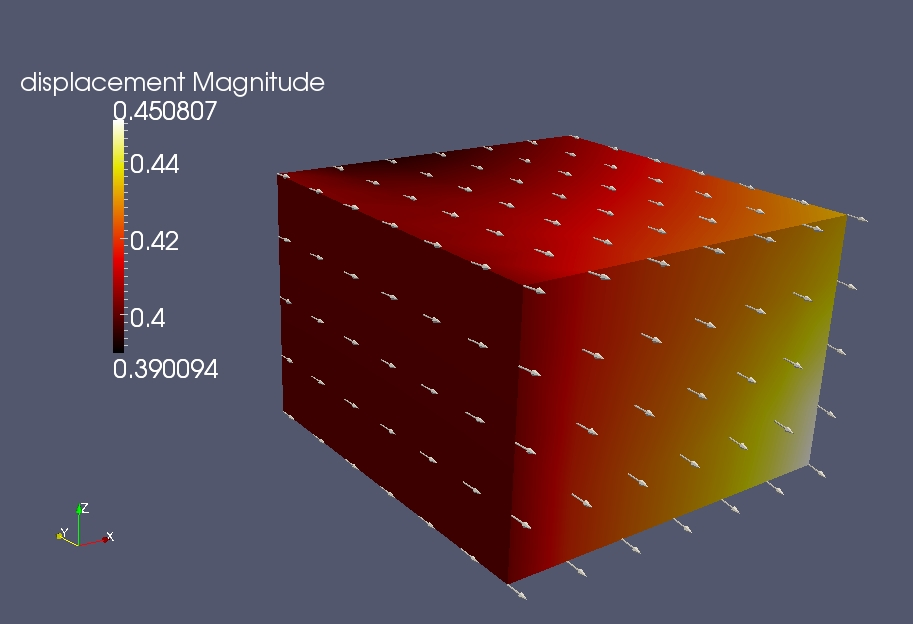
\includegraphics[width=10cm]{examples/figs/3dhex8_step05-displ-t40}
  \caption{Displacement field for example step05 at t = 40 years visualized using
    ParaView. The mesh has been distorted by the computed displacements
    (magnified by 500), and the vectors show the computed displacements.}
  \label{fig:example:3dhex8:step05:displacement}
\end{figure}


\subsubsection{Step06 - Dirichlet Boundary Conditions with Time-Dependent Kinematic Fault Slip}

The \filename{step06.cfg} file defines a problem with Dirichlet (displacement)
boundary conditions corresponding to zero x- and y-displacements applied
on the negative and positive x-faces and a vertical fault that includes
multiple earthquake ruptures as well as steady fault creep. The upper
(locked) portion of the fault has 4 m of left-lateral slip every 200
years, while the lower (creeping) portion of the fault slips at a
steady rate of 2 cm/year. The problem bears some similarity to the
strike-slip fault model of Savage and Prescott \cite{Savage:Prescott:1978},
except that the fault creep extends through the viscoelastic portion
of the domain, and the far-field displacement boundary conditions
are held fixed.

In this example and the remainder of the examples in this section,
we change the time stepping behavior from the default \object{TimeStepUniform}
to \object{TimeStepAdapt}. For adaptive time stepping, we provide
the maximum permissible time-step size, along with a stability factor.
The stability factor controls the time-step size relative to the stable
time-step size provided by the different materials in the model. A
\property{stability\_factor} of 1.0 means we should use the stable time-step
size, while a \property{stability\_factor} greater than 1.0 means we
want to use a smaller time-step size. A \property{stability\_factor}
less than 1.0 allows time-step sizes greater than the stable time-step
size, which may provide inaccurate results. The adaptive time stepping
information is provided as:
\begin{cfg}
# Change time stepping algorithm from uniform time step, to adaptive
# time stepping.
<f>time_step</f> = pylith.problems.TimeStepAdapt

# Change the total simulation time to 700 years, and set the maximum time
# step size to 10 years.
<h>[pylithapp.timedependent.implicit.time_step]</h>
<p>total_time</p> = 700.0*year
<p>max_dt</p> = 10.0*year
<p>stability_factor</p> = 1.0 ; use time step equal to stable value from materials
\end{cfg}
In this example and the remainder of the examples in this section,
we also make use of HDF5 output rather than the default VTK output.
HDF5 output is a new feature beginning with PyLith version 1.6, and
it is much more efficient with the additional advantage that multiple
time steps can be contained in a single file. PyLith also produces
Xdmf files describing the contents of the HDF5 files, which allows
the files to be read easily by applications such as ParaView. Since
VTK output is still the default, we must change the value from the
default. Also note that the filename suffix is \filename{h5}:
\begin{cfg}
# Give basename for output of solution over domain.
<h>[pylithapp.problem.formulation.output.domain]</h>
# We specify that output occurs in terms of a given time frequency, and
# ask for output every 50 years.
<p>output_freq</p> = time_step
<p>time_step</p> = 50.0*year

# We are using HDF5 output so we must change the default writer.
<f>writer</f> = pylith.meshio.DataWriterHDF5
<p>writer.filename</p> = output/step06.h5  
\end{cfg}
Note that we no longer need the \property{writer.time\_format} or
\property{writer.time\_constant} properties, since all time steps are
contained in a single file. The HDF5 writer does not have these
properties, so if we attempt to define them an error will result.

We also set the writer for other output as well, since it is not the
default. For subdomain output we use:
\begin{cfg}
# Give basename for output of solution over ground surface.
<h>[pylithapp.problem.formulation.output.subdomain]</h>
# Name of nodeset for ground surface.
<p>label</p> = face_zpos

# We keep the default output frequency behavior (skip every n steps), and
# ask to skip 0 steps between output, so that we get output every time step.
# We again switch the writer to produce HDF5 output.
<p>skip</p> = 0
<f>writer</f> = pylith.meshio.DataWriterHDF5
<p>writer.filename</p> = output/step06-groundsurf.h5  

# Fault output
<h>[pylithapp.problem.interfaces.fault.output]</h>
# We keep the default output frequency behavior (skip every n steps), and
# ask to skip 0 steps between output, so that we get output every time step.
# We again switch the writer to produce HDF5 output.
<p>skip</p> = 0
<f>writer</f> = pylith.meshio.DataWriterHDF5
<p>writer.filename</p> = output/step06-fault.h5
\end{cfg}
Due to the simplicity of the boundary conditions, we are able to use
the default \object{ZeroDispBC} for the positive and negative x-faces,
as well as the negative z-face. As for example step03, we define a
fault interface, we identify the nodeset corresponding to the fault,
and we provide quadrature information for the fault. We then define
an array of earthquake sources and provide an origin time for each:
\begin{cfg}
<h>[pylithapp.timedependent.interfaces.fault]</h>
# Set earthquake sources to an array consisting of creep and 3 ruptures.
<f>eq_srcs</f> = [creep, one, two, three]
<p>eq_srcs.creep.origin_time</p> = 00.0*year
<p>eq_srcs.one.origin_time</p> = 200.0*year
<p>eq_srcs.two.origin_time</p> = 400.0*year
<p>eq_srcs.three.origin_time</p> = 600.0*year
\end{cfg}
Note that the creep begins at t = 0 years, while the ruptures (\facility{one},
\facility{two}, \facility{three}) occur at regular intervals of 200 years.
We retain the default \object{StepSlipFn} for the ruptures. Each of
the ruptures has the same amount of slip, and slip occurs simultaneously
for the entire rupture region, so we can use the same \object{SimpleDB}
files providing slip and slip time for each rupture:
\begin{cfg}
# Define slip and origin time for first rupture.
<h>[pylithapp.timedependent.interfaces.fault.eq_srcs.one.slip_function]</h>
<p>slip.iohandler.filename</p> = spatialdb/finalslip_rupture.spatialdb
<p>slip_time.iohandler.filename</p> = spatialdb/sliptime.spatialdb

# Define slip and origin time for second rupture.
<h>[pylithapp.timedependent.interfaces.fault.eq_srcs.two.slip_function]</h>
<p>slip.iohandler.filename</p> = spatialdb/finalslip_rupture.spatialdb
<p>slip_time.iohandler.filename</p> = spatialdb/sliptime.spatialdb

# Define slip and origin time for third rupture.
<h>[pylithapp.timedependent.interfaces.fault.eq_srcs.three.slip_function]</h>
<p>slip.iohandler.filename</p> = spatialdb/finalslip_rupture.spatialdb
<p>slip_time.iohandler.filename</p> = spatialdb/sliptime.spatialdb
\end{cfg}
For the creep source, we change the slip function to \object{ConstRateSlipFn},
and we use a \object{SimpleDB} for both the slip time and the slip
rate:
\begin{cfg}
# Define slip rate and origin time for fault creep.
<h>[pylithapp.timedependent.interfaces.fault.eq_srcs.creep]</h>
<f>slip_function</f> = pylith.faults.ConstRateSlipFn
<p>slip_function.slip_rate.iohandler.filename</p> = spatialdb/sliprate_creep.spatialdb
<p>slip_function.slip_time.iohandler.filename</p> = spatialdb/sliptime.spatialdb
\end{cfg}
For all earthquake sources we provide both an \property{origin\_time}
and a \property{slip\_function.slip\_time}. The first provides the starting
time for the entire earthquake source, while the second provides any
spatial variation in the slip time with respect to the \property{origin\_time}
(if any). Since there are multiple earthquake sources of different
types, there are a number of additional fault information fields available
for output. We add these additional fields' output to the fault information
file:
\begin{cfg}
<h>[pylithapp.timedependent.interfaces.fault]</h>
<p>output.vertex_info_fields</p> = [normal_dir, strike_dir, dip_dir, final_slip_creep, \
  final_slip_one, final_slip_two, final_slip_three, slip_time_creep, slip_time_one, \
  slip_time_two, slip_time_three]
\end{cfg}
This additional information will be contained in file \filename{step06-fault\_info.h5}.
It will contain final slip information for each earthquake source
along with slip time information. When we have run the simulation,
the output HDF5 and Xdmf files will be contained in \filename{examples/3d/hex8/output}
(all with a prefix of \filename{step06}). To open the files in ParaView,
the Xdmf (\filename{xmf}) files should be opened, as these files describe
the HDF5 data structure. Results using ParaView are shown in Figure
\vref{fig:example:3dhex8:step06:displacement}.

\begin{figure}
  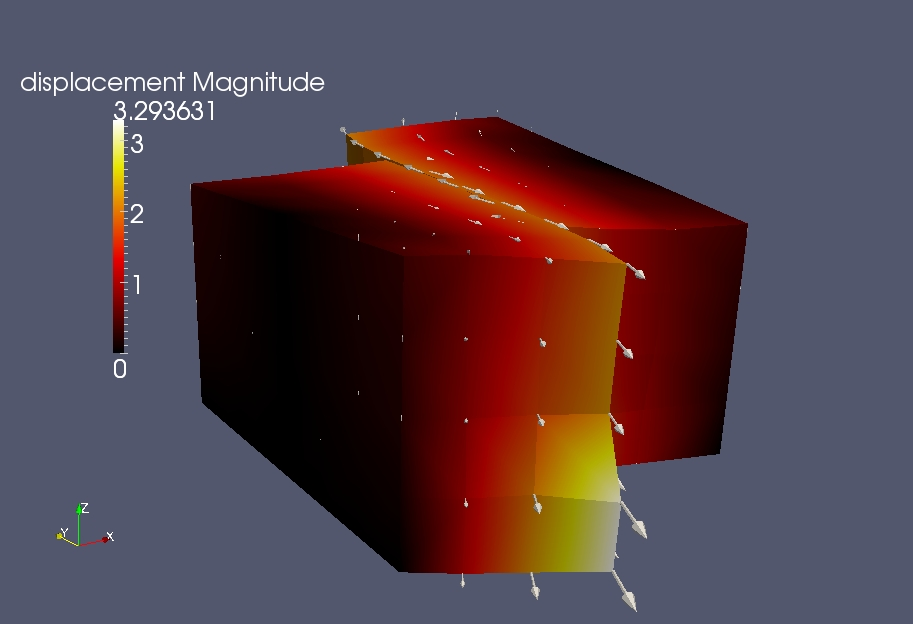
\includegraphics[width=10cm]{examples/figs/3dhex8_step06-displ-t300}
  \caption{Displacement field for example step06 at t = 300 years visualized
    using ParaView. The mesh has been distorted by the computed displacements
    (magnified by 500), and the vectors show the computed displacements.}
  \label{fig:example:3dhex8:step06:displacement}
\end{figure}


\subsubsection{Step07 - Dirichlet Velocity Boundary Conditions with Time-Dependent Kinematic Fault Slip}

In step07 we add velocity boundary conditions in the positive and
negative y-directions on the positive and negative x-faces, so that
the external boundaries keep pace with the average fault slip. This
problem is nearly identical to the strike-slip fault model of Savage
and Prescott \cite{Savage:Prescott:1978}, except that the fault creep
extends through the viscoelastic portion of the domain.

We use the default \object{ZeroDispBC} for the initial displacements
on the positive and negative x-faces, as well as the negative z-face.
For the velocities on the positive and negative x-faces, we use a
\object{UniformDB}:
\begin{cfg}
# Boundary condition on +x face
[pylithapp.timedependent.bc.x_pos]
<p>bc_dof</p> = [0, 1]
<p>label</p> = face_xpos
<p>db_initial.label</p> = Dirichlet BC on +x
<f>db_rate</f> = spatialdata.spatialdb.UniformDB
<p>db_rate.label</p> = Dirichlet rate BC on +x
<p>db_rate.values</p> = [displacement-rate-x, displacement-rate-y, rate-start-time]
<p>db_rate.data</p> = [0.0*cm/year, 1.0*cm/year, 0.0*year]

# Boundary condition on -x face
<h>[pylithapp.timedependent.bc.x_neg]</h>
<p>bc_dof</p> = [0, 1]
<p>label</p> = face_xneg
<p>db_initial.label</p> = Dirichlet BC on -x
<f>db_rate</f> = spatialdata.spatialdb.UniformDB
<p>db_rate.label</p> = Dirichlet rate BC on +x
<p>db_rate.values</p> = [displacement-rate-x, displacement-rate-y, rate-start-time]
<p>db_rate.data</p> = [0.0*cm/year, -1.0*cm/year, 0.0*year]
\end{cfg}
The fault definition information is identical to example \filename{step06}.
In previous examples, we have just used the default output for the
domain and subdomain (ground surface), which includes the displacements.
In many cases, it is also useful to include the velocities. PyLith
provides this information, computing the velocities for the current
time step as the difference between the current displacements and
the displacements from the previous time step, divided by the time-step
size. This is more accurate than computing the velocities from the
displacement field output that has been decimated in time. We can
obtain this information by explicitly requesting it in \property{vertex\_data\_fields}:
\begin{cfg}
# Give basename for output of solution over domain.
<h>[pylithapp.problem.formulation.output.domain]</h>
# We specify that output occurs in terms of a given time frequency, and
# ask for output every 50 years.
# We also request velocity output in addition to displacements.
<p>vertex_data_fields</p> = [displacement, velocity]
<p>output_freq</p> = time_step
<p>time_step</p> = 50.0*year

# We are using HDF5 output so we must change the default writer.
<f>writer</f> = pylith.meshio.DataWriterHDF5
<p>writer.filename</p> = output/step07.h5

# Give basename for output of solution over ground surface.
<h>[pylithapp.problem.formulation.output.subdomain]</h>
# Name of nodeset for ground surface.
<p>label</p> = face_zpos

# We also request velocity output in addition to displacements.
<p>vertex_data_fields</p> = [displacement, velocity]
# We keep the default output frequency behavior (skip every n steps), and
# ask to skip 0 steps between output, so that we get output every time step.
<p>skip</p> = 0

# We again switch the writer to produce HDF5 output.
<f>writer</f> = pylith.meshio.DataWriterHDF5
<p>writer.filename</p> = output/step07-groundsurf.h5
\end{cfg}
When we have run the simulation, the output HDF5 and Xdmf files will
be contained in \filename{examples/3d/hex8/output} (all with a prefix
of \filename{step07}). As for example step06, make sure to open the
\filename{xmf} files rather than the \filename{h5} files. Results using
ParaView are shown in Figure \vref{fig:example:3dhex8:step07:displacement}.

\begin{figure}
  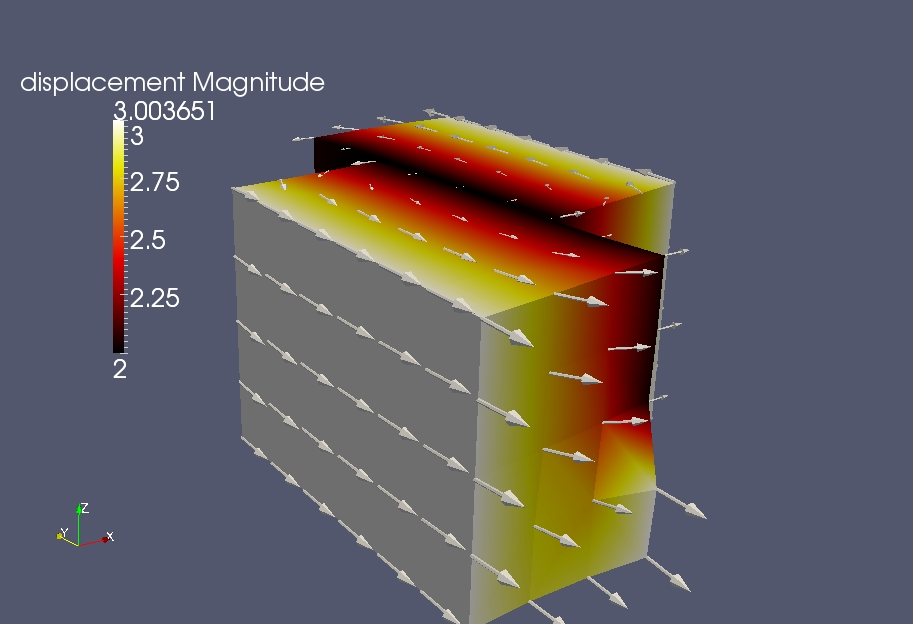
\includegraphics[width=10cm]{examples/figs/3dhex8_step07-displ-vel-t300}
  \caption{Displacement field (color contours) and velocity field (vectors) for
    example step07 at t = 300 years visualized using ParaView. The mesh
    has been distorted by the computed displacements (magnified by 500),
    and the vectors show the computed velocities.}
  \label{fig:example:3dhex8:step07:displacement}
\end{figure}


\subsubsection{Step08 - Dirichlet Velocity Boundary Conditions with Time-Dependent Kinematic Fault Slip and Power-Law Rheology}
\label{sec:example:3dhex8:step08}

The \filename{step08.cfg} file defines a problem that is identical to
example step07, except the the lower crust is composed of a power-law
viscoelastic material. Since the material behavior is now nonlinear,
we must use the nonlinear solver:
\begin{cfg}
<h>[pylithapp.timedependent]</h>
# For this problem we must switch to a nonlinear solver.
<f>implicit.solver</f> = pylith.problems.SolverNonlinear
\end{cfg}
Although we have not discussed the PyLith PETSc settings previously,
note that the use of the nonlinear solver may require additional options
if we wish to override the defaults. These settings are contained
in \filename{pylithapp.cfg}:
\begin{cfg}
<h>[pylithapp.petsc]</h>
# Nonlinear solver monitoring options.
<p>snes_rtol</p> = 1.0e-8
<p>snes_atol</p> = 1.0e-12
<p>snes_max_it</p> = 100
<p>snes_monitor</p> = true
<p>snes_view</p> = true
<p>snes_converged_reason</p> = true
\end{cfg}
These settings are ignored unless we are using the nonlinear solver.

When setting the physical properties for the power-law material in
PyLith, the parameters (see Section
\vref{sec:materials:formulation:powerlaw}) do not generally correspond
to the values provided in laboratory results.  PyLith includes a
utility code, \filename{powerlaw\_gendb.py}, to simplify the process
of using laboratory results with PyLith. This utility code is
installed in the same location as PyLith. An example of how to use it
is in \filename{examples/3d/hex8/spatialdb/powerlaw}. The user must
provide a spatial database defining the spatial distribution of
laboratory-derived parameters (contained in
\filename{powerlaw\_params.spatialdb}), another spatial database
defining the temperature field in degrees K (contained in
\filename{temperature.spatialdb}), and a set of points for which
values are desired (\filename{powerlaw\_points.txt}).  The parameters
for the code are defined in \filename{powerlaw\_gendb.cfg}.  The
properties expected by PyLith are \texttt{reference\_strain\_rate},
\texttt{reference\_stress}, and \texttt{power\_law\_exponent}. The
user must specify either \texttt{reference\_strain\_rate} or
\texttt{reference\_stress} so that \filename{powerlaw\_gendb.py} can
compute the other property.  Default values of 1.0e-6 1/s and 1 MPa
are provided. In this example, the same database was used for all
parameters, and a separate database was used to define the temperature
distribution. In practice, the user can provide any desired thermal
model to provide the spatial database for the temperature. In this
example, a simple 1D (vertically-varying) distribution was used. The
utility code can be used by simply executing it from the
\filename{examples/3d/hex8/spatialdb/powerlaw} directory:
\begin{shell}
$ powerlaw_gendb.py
\end{shell}
This code will automatically read the parameters in \filename{powerlaw\_gendb.cfg}
in creating the file \filename{examples/3d/hex8/spatialdb/mat\_powerlaw.spatialdb}.

We first change the material type of the lower crust to \object{PowerLaw3D}:
\begin{cfg}
# Change material type of lower crust to power-law viscoelastic.
<h>[pylithapp.timedependent]</h>
<f>materials.lower_crust</f> = pylith.materials.PowerLaw3D
\end{cfg}
In many cases, it is useful to obtain the material properties from two
different sources. For example, the elastic properties may come from a
seismic velocity model while the viscous properties may be derived
from a thermal model. In such a case we can use a
\object{CompositeDB}, which allows a different spatial database to be
used for a subset of the properties. We do this as follows:
\begin{cfg}
# Provide a spatial database from which to obtain property values.
# In this case, we prefer to obtain the power-law properties from one
# database and the elastic properties from another database, so we use
# a CompositeDB. Each part of the CompositeDB is a SimpleDB.
<h>[pylithapp.timedependent.materials.lower_crust]</h>
<f>db_properties</f> = spatialdata.spatialdb.CompositeDB
<f>db_properties.db_A</f> = spatialdata.spatialdb.SimpleDB
<f>db_properties.db_B</f> = spatialdata.spatialdb.SimpleDB
\end{cfg}
We must define the properties that come from each spatial database
and then provide the database parameters:
\begin{cfg}
# Provide the values to be obtained from each database and the database
# name.
<h>[pylithapp.timedependent.materials.lower_crust.db_properties]</h>
<p>values_A</p> = [density, vs, vp]   ; Elastic properties.
<p>db_A.label</p> = Elastic properties
<p>db_A.iohandler.filename</p> = spatialdb/mat_elastic.spatialdb
<p>values_B</p> = [reference-stress, reference-strain-rate, power-law-exponent] ; Power-law properties.
<p>db_B.label</p> = Power-law properties
<p>db_B.iohandler.filename</p> = spatialdb/mat_powerlaw.spatialdb
\end{cfg}
The \object{PowerLaw3D} material has additional properties and state
variables with respect to the default \object{ElasticIsotropic3D}
material, so we request that these properties be written to the \facility{lower\_crust}
material files:
\begin{cfg}
# Since there are additional properties and state variables for the
# power-law model, we explicitly request that they be output. Properties are
# named in cell_info_fields and state variables are named in
# cell_data_fields.
<h>[pylithapp.timedependent.materials.lower_crust]</h>
<p>output.cell_info_fields</p> = [density, mu, lambda, reference_strain_rate, reference_stress, power_law_exponent]
<p>output.cell_data_fields</p> = [total_strain, stress, viscous_strain]
\end{cfg}
When we have run the simulation, the output HDF5 and Xdmf files will
be contained in \filename{examples/3d/hex8/output} (all with a prefix
of \filename{step08}). Results using ParaView are shown in Figure
\vref{fig:example:3dhex8:step8:displacement}.

\begin{figure}
  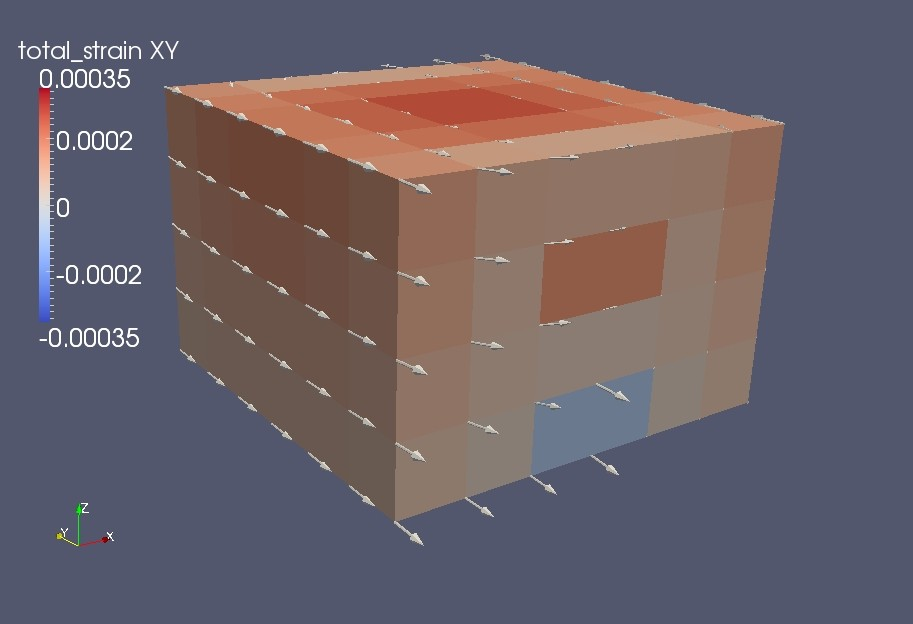
\includegraphics[width=10cm]{examples/figs/3dhex8_step08-strain-displ-t150}
  \caption{The XY-component of strain (color contours) and displacement field
    (vectors) for example step08 at t = 150 years visualized using ParaView.
    For this visualization, we loaded both the \filename{step08-lower\_crust.xmf}
    and \filename{step08-upper\_crust.xmf} files to contour the strain field,
    and superimposed on it the displacement field vectors from \filename{step08.xmf}.}
  \label{fig:example:3dhex8:step8:displacement}
\end{figure}


\subsubsection{Step09 - Dirichlet Velocity Boundary Conditions with Time-Dependent
Kinematic Fault Slip and Drucker-Prager Elastoplastic Rheology}

In this example we use a Drucker-Prager elastoplastic rheology in
the lower crust. As in example step08, the material behavior is nonlinear
so we again use the nonlinear solver. The material is elastoplastic,
there is no inherent time-dependent response and the stable time-step
size for the material depends on the loading conditions. To avoid
this, we set the maximum time-step size to 5 years rather than the
value of 10 years used in example \filename{step08}:
\begin{cfg}
# Change the total simulation time to 700 years, and set the maximum time
# step size to 5 years.
<h>[pylithapp.timedependent.implicit.time_step]</h>
<p>total_time</p> = 700.0*year
<p>max_dt</p> = 5.0*year
<p>stability_factor</p> = 1.0 ; use time step equal to stable value from materials

# For this problem we set adapt\_skip to zero so that the time step size is
# readjusted every time step.
<p>adapt_skip</p> = 0

# Change material type of lower crust to Drucker-Prager.
<h>[pylithapp.timedependent]</h>
<f>materials.lower_crust</f> = pylith.materials.DruckerPrager3D

# Provide a spatial database from which to obtain property values.
# In this case, we prefer to obtain the Drucker-Prager properties from one
# database and the elastic properties from another database, so we use
# a CompositeDB. Each part of the CompositeDB is a SimpleDB.
<h>[pylithapp.timedependent.materials.lower_crust]</h>
<f>db_properties</f> = spatialdata.spatialdb.CompositeDB
<f>db_properties.db_A</f> = spatialdata.spatialdb.SimpleDB
<f>db_properties.db_B</f> = spatialdata.spatialdb.SimpleDB
\end{cfg}
As for the step08 example, we first define the properties that come
from each spatial database and then provide the database filename:
\begin{cfg}
# Provide the values to be obtained from each database and the database
# name.
<h>[pylithapp.timedependent.materials.lower_crust.db_properties]</h>
<p>values_A</p> = [density,vs,vp] ; Elastic properties.
<p>db_A.label</p> = Elastic properties
<p>db_A.iohandler.filename</p> = spatialdb/mat_elastic.spatialdb

<p>values_B</p> = [friction-angle, cohesion, dilatation-angle] ; Drucker-Prager properties.
<p>db_B.label</p> = Drucker-Prager properties
<p>db_B.iohandler.filename</p> = spatialdb/mat\_druckerprager.spatialdb
\end{cfg}
We also request output of the properties and state variables that
are unique to the \object{DruckerPrager3D} material:
\begin{cfg}
# Since there are additional properties and state variables for the
# Drucker-Prager model, we explicitly request that they be output.
# Properties are named in cell\_info\_fields and state variables are named in
# cell_data_fields.
<h>[pylithapp.timedependent.materials.lower_crust]</h>
<p>output.cell_info_fields</p> = [density, mu, lambda, alpha_yield, beta, alpha_flow]
<p>output.cell_data_fields</p> = [total_strain, stress, plastic_strain]
\end{cfg}
When we have run the simulation, the output HDF5 and Xdmf files will
be contained in \filename{examples/3d/hex8/output} (all with a prefix
of \filename{step09}). Results using ParaView are shown in Figure
\vref{fig:example:3dhex8:step09:displacement}.

\begin{figure}
  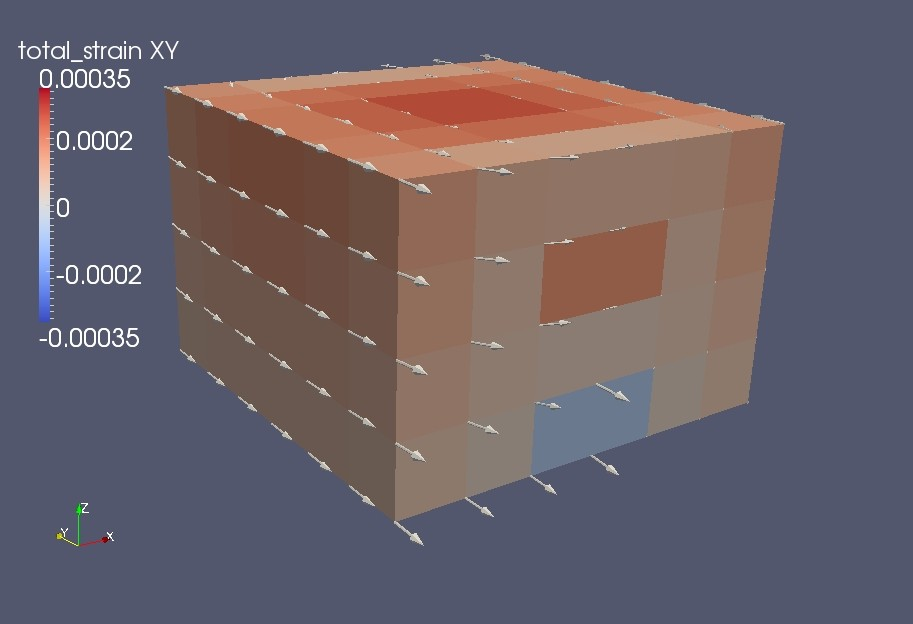
\includegraphics[width=10cm]{examples/figs/3dhex8_step08-strain-displ-t150}
  \caption{The XY-component of strain (color contours) and displacement field
    (vectors) for example step09 at t = 150 years visualized using ParaView.
    For this visualization, we loaded both the \filename{step09-lower\_crust.xmf}
    and \filename{step09-upper\_crust.xmf} files to contour the strain field,
    and superimposed on it the displacement field vectors from \filename{step09.xmf}.}
  \label{fig:example:3dhex8:step09:displacement}
\end{figure}

% End of file


\subsection{\label{sec:Tutorial-3d-hex8-friction}Fault Friction Examples}

PyLith features discussed in this tutorial:
\begin{itemize}
\item Static fault friction
\item Slip-weakening fault friction
\item Rate-and-state fault friction
\item Nonlinear solver
\end{itemize}

\subsubsection{Overview}

This set of examples provides an introduction to using fault friction
in static and quasi-static problems with PyLith. Dynamic problems
with fault friction are discussed in Section \vref{sec:tutorial:shearwave:quad4}.
The boundary conditions are all either static or quasi-static Dirichlet
conditions, and only elastic materials are used. In all the fault
friction examples we apply axial (x) displacements on both the positive
and negative x-faces to maintain a compressive normal tractions on
the fault. Otherwise, there would be no frictional resistance. Fault
friction generates nonlinear behavior, so we use the nonlinear solver.
All of the examples are contained in the directory \texttt{examples/3d/hex8},
and the corresponding \texttt{.cfg} files are \texttt{step10.cfg},
\texttt{step11.cfg}, \texttt{step12.cfg}, \texttt{step13.cfg}, and
\texttt{step14.cfg}. Each example may be run as follows:
\begin{lyxcode}
pylith~stepXX.cfg
\end{lyxcode}
This will cause PyLith to read the default parameters in \texttt{pylithapp.cfg},
and then override or augment them with the additional parameters in
the \texttt{stepXX.cfg} file. Each \texttt{.cfg} file is extensively
documented, to provide detailed information on the various parameters.


\subsubsection{Step10 - Static Friction (Stick) with Static Dirichlet Boundary Conditions}

The \texttt{step10.cfg} file defines a problem that is identical to
example step01, except for the presence of a vertical fault with static
friction. In this case, the applied displacements are insufficient
to cause the fault to slip, so the solution is identical to that in
example step01. As in previous examples involving faults, we must
first provide an array defining the fault interfaces:
\begin{lyxcode}
{[}pylithapp.timedependent{]}

\#~Set~interfaces~to~an~array~of~1~fault:~'fault'.

interfaces~=~{[}fault{]}
\end{lyxcode}
Since all fault friction models are nonlinear we must also use the
nonlinear solver:
\begin{lyxcode}
{[}pylithapp.timedependent.implicit{]}

\#~Fault~friction~is~a~nonlinear~problem~so~we~need~to~use~the~nonlinear

\#~solver.

solver~=~pylith.problems.SolverNonlinear
\end{lyxcode}
We need to change the fault interface from the default (\texttt{FaultCohesiveKin})
to \texttt{FaultCohesiveDyn} and we set the friction model to use:
\begin{lyxcode}
{[}pylithapp.timedependent.interfaces{]}

\#~Change~fault~to~dynamic~fault~interface.

fault~=~pylith.faults.FaultCohesiveDyn~\\
~\\


{[}pylithapp.timedependent.interfaces.fault{]}

\#~Use~the~static~friction~model.

friction~=~pylith.friction.StaticFriction
\end{lyxcode}
The \texttt{StaticFriction} model requires values for the coefficient
of friction and the cohesion (see Section \vref{sec:fault:constitutive:models}).
We provide both of these using a \texttt{UniformDB}:
\begin{lyxcode}
{[}pylithapp.timedependent.interfaces.fault{]}

\#~Set~static~friction~model~parameters~using~a~uniform~DB.~Set~the

\#~static~coefficient~of~friction~to~0.6~and~cohesion~to~0.0~Pa.

friction.db\_properties~=~spatialdata.spatialdb.UniformDB

friction.db\_properties.label~=~Static~friction

friction.db\_properties.values~=~{[}friction-coefficient,cohesion{]}

friction.db\_properties.data~=~{[}0.6,0.0{*}Pa{]}
\end{lyxcode}
Fault friction models require additional PETSc settings:
\begin{lyxcode}
\#~NOTE:~There~are~additional~settings~specific~to~fault~friction.

{[}pylithapp.petsc{]}

\#~Friction~sensitivity~solve~used~to~compute~the~increment~in~slip

\#~associated~with~changes~in~the~Lagrange~multiplier~imposed~by~the

\#~fault~constitutive~model.

friction\_pc\_type~=~asm

friction\_sub\_pc\_factor\_shift\_type~=~nonzero

friction\_ksp\_max\_it~=~25

friction\_ksp\_gmres\_restart~=~30

\#~Uncomment~to~view~details~of~friction~sensitivity~solve.

\#friction\_ksp\_monitor~=~true

\#friction\_ksp\_view~=~true

friction\_ksp\_converged\_reason~=~true


\end{lyxcode}
When we have run the simulation, the output VTK files will be contained
in \texttt{examples/3d/hex8/output} (all with a pvrefix of \texttt{step10}).
Results using ParaView are shown in Figure \vref{fig:step10-fault-traction-slip}.

\begin{figure}
\begin{centering}
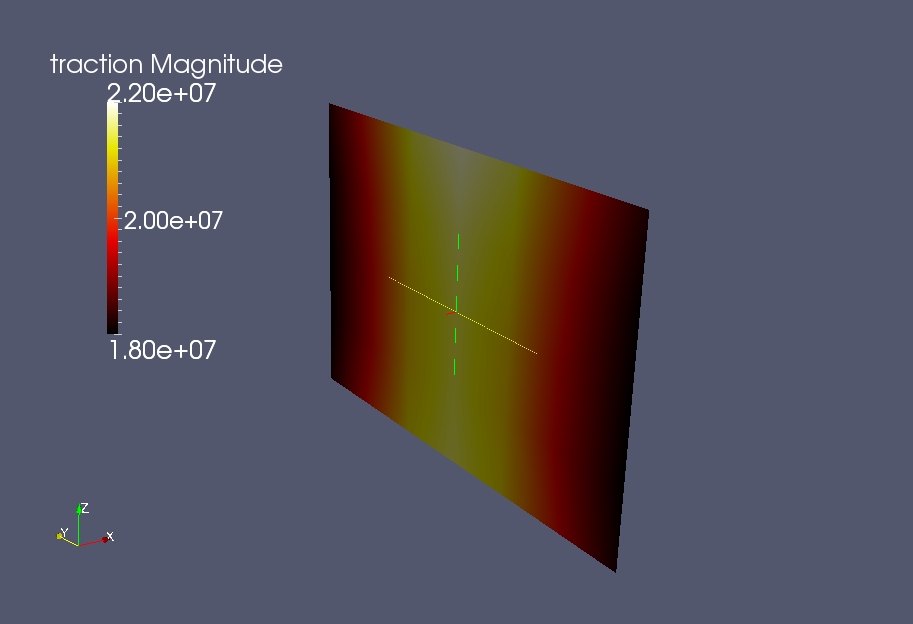
\includegraphics[width=10cm]{tutorials/3dhex8/figs/step10-fault-traction-slip}
\par\end{centering}

\caption{Magnitude of tractions on the fault for example step10 visualized
using ParaView. \label{fig:step10-fault-traction-slip}}
\end{figure}



\subsubsection{Step11 - Static Friction (Slip) with Static Dirichlet Boundary Conditions}

In step11 we apply twice as much shear displacement as in step10,
which is sufficient to induce slip on the fault. All other settings
are identical. To change the amount of shear displacement, we change
the spatial database for the positive and negative x-faces to a \texttt{UniformDB},
and apply the altered values within the \texttt{.cfg} file:
\begin{lyxcode}
\#~+x~face

{[}pylithapp.timedependent.bc.x\_pos{]}

bc\_dof~=~{[}0,~1{]}

label~=~face\_xpos

db\_initial~=~spatialdata.spatialdb.UniformDB

db\_initial.label~=~Dirichlet~BC~on~+x

db\_initial.values~=~{[}displacement-x,displacement-y{]}

db\_initial.data~=~{[}-1.0{*}m,2.0{*}m{]}



\#~-x~face

{[}pylithapp.timedependent.bc.x\_neg{]}

bc\_dof~=~{[}0,~1{]}

label~=~face\_xneg

db\_initial~=~spatialdata.spatialdb.UniformDB

db\_initial.label~=~Dirichlet~BC~on~-x

db\_initial.values~=~{[}displacement-x,displacement-y{]}

db\_initial.data~=~{[}1.0{*}m,-2.0{*}m{]}
\end{lyxcode}
When we have run the simulation, the output VTK files will be contained
in \texttt{examples/3d/hex8/output} (all with a pvrefix of \texttt{step11}).
Results using ParaView are shown in Figure \vref{fig:step11-fault-traction-slip}.

\begin{figure}
\begin{centering}
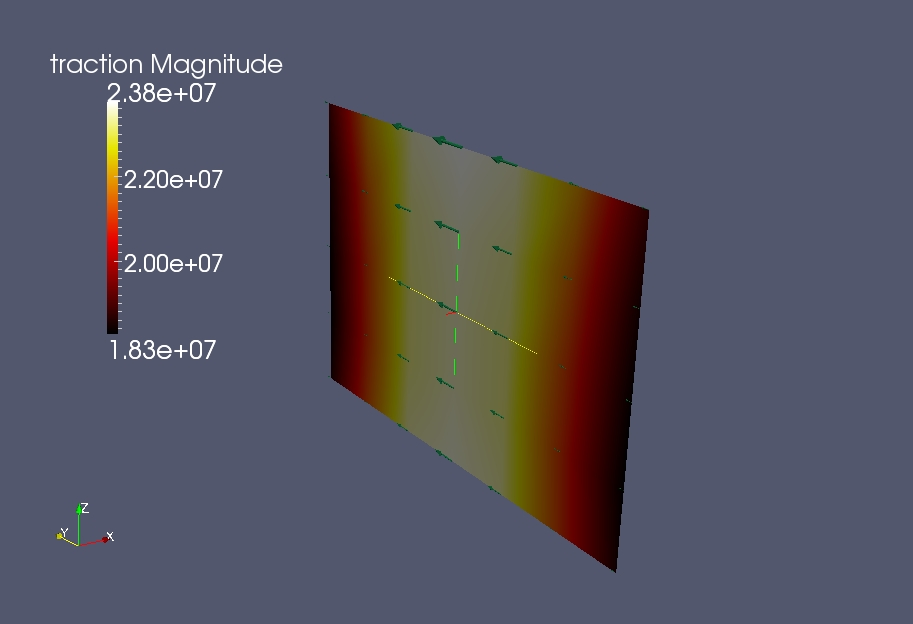
\includegraphics[width=10cm]{tutorials/3dhex8/figs/step11-fault-traction-slip}
\par\end{centering}

\caption{Magnitude of tractions on the fault for example step10 visualized
using ParaView. Vectors of fault slip are also plotted. Note that
PyLith outputs slip in the fault coordinate system, so we transform
them to the global coordinate system using the Calculator in ParaView.
A more general approach involves outputing the fault coordinate system
information and using these fields in the Calculator. \label{fig:step11-fault-traction-slip}}
\end{figure}



\subsubsection{Step12 - Static Friction with Quasi-Static Dirichlet Boundary Conditions}

The \texttt{step12.cfg} file describes a problem that is similar to
examples step10 and step11, except that we apply velocity boundary
conditions and run the simulation for 200 years. Once fault friction
is overcome, the fault slips at a steady rate. To prevent convergence
problems we set the time step size to a constant value of 5 years:
\begin{lyxcode}
\#~Change~the~total~simulation~time~to~200~years,~and~use~a~constant~time

\#~step~size~of~5~years.

{[}pylithapp.timedependent.implicit.time\_step{]}

total\_time~=~200.0{*}year

dt~=~5.0{*}year
\end{lyxcode}
As in the other fault friction examples, we apply initial displacements
along the x-axis (to maintain a compressive stress on the fault),
and we apply velocity boundary conditions that yield a left-lateral
sense of motion:
\begin{lyxcode}
\#~+x~face~-{}-~Dirichlet

{[}pylithapp.timedependent.bc.x\_pos{]}

bc\_dof~=~{[}0,1{]}

label~=~face\_xpos

db\_initial~=~spatialdata.spatialdb.UniformDB

db\_initial.label~=~Dirichlet~BC~on~+x

db\_initial.values~=~{[}displacement-x,displacement-y{]}

db\_initial.data~=~{[}-1.0{*}m,0.0{*}m{]}

db\_rate~=~spatialdata.spatialdb.UniformDB

db\_rate.label~=~Dirichlet~rate~BC~on~+x

db\_rate.values~=~{[}displacement-rate-x,displacement-rate-y,rate-start-time{]}

db\_rate.data~=~{[}0.0{*}cm/year,1.0{*}cm/year,0.0{*}year{]}~\\
~\\


\#~-x~face

{[}pylithapp.timedependent.bc.x\_neg{]}

bc\_dof~=~{[}0,~1{]}

label~=~face\_xneg

db\_initial.label~=~Dirichlet~BC~on~-x

db\_rate~=~spatialdata.spatialdb.UniformDB

db\_rate.label~=~Dirichlet~rate~BC~on~-x

db\_rate.values~=~{[}displacement-rate-x,displacement-rate-y,rate-start-time{]}

db\_rate.data~=~{[}0.0{*}cm/year,-1.0{*}cm/year,0.0{*}year{]}
\end{lyxcode}
For this example, we keep the same coefficient of friction as examples
step10 and step11, but we include a cohesion of 2 MPa:
\begin{lyxcode}
{[}pylithapp.timedependent.interfaces.fault{]}

\#~Set~static~friction~model~parameters~using~a~uniform~DB.~Set~the

\#~static~coefficient~of~friction~to~0.6~and~cohesion~to~2.0~MPa.

friction.db\_properties~=~spatialdata.spatialdb.UniformDB

friction.db\_properties.label~=~Static~friction

friction.db\_properties.values~=~{[}friction-coefficient,cohesion{]}

friction.db\_properties.data~=~{[}0.6,2.0{*}MPa{]}
\end{lyxcode}
When we have run the simulation, the output VTK files will be contained
in \texttt{examples/3d/hex8/output} (all with a pvrefix of \texttt{step12}).
Results using ParaView are shown in Figure \vref{fig:step12-displ-t200}.

\begin{figure}
\begin{centering}
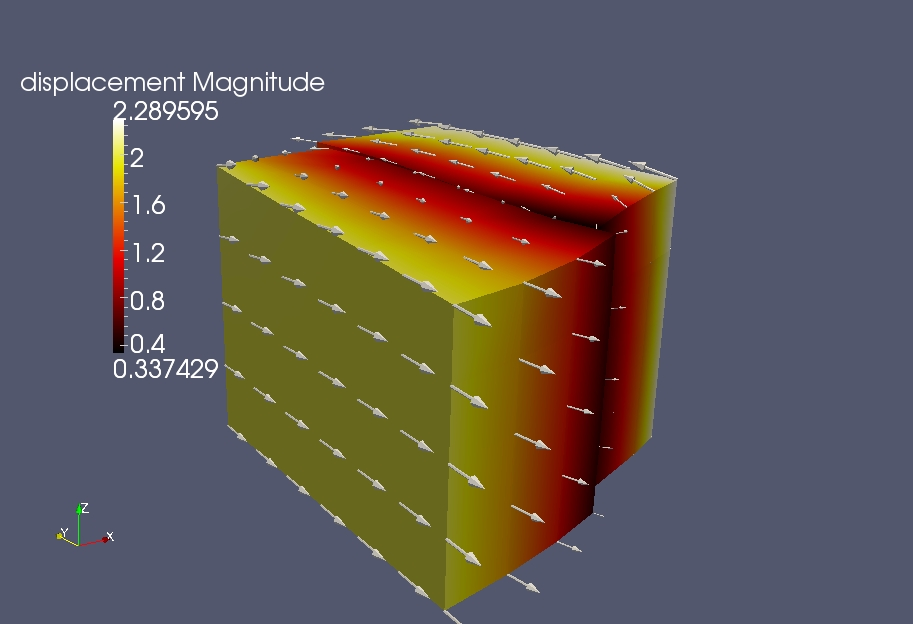
\includegraphics[width=10cm]{tutorials/3dhex8/figs/step12-displ-t200}
\par\end{centering}

\caption{Displacement field for example step12 at t = 200 years visualized
using ParaView. The mesh has been distorted by the computed displacements
(magnified by 500), and the vectors show the computed displacements.\label{fig:step12-displ-t200}}
\end{figure}



\subsubsection{Step13 - Slip-Weakening Friction with Quasi-Static Dirichlet Boundary
Conditions}

In this example we replace the static friction fault constitutive
model in step12 with a slip-weakening friction fault constitutive
model. Fault friction is overcome at about t = 80 years, the fault
slips in each subsequent time step. We again use a constant time step
size of 5 years and apply the same intial displacement and velocity
boundary conditions.

We first define the friction model for the simulation:
\begin{lyxcode}
{[}pylithapp.timedependent.interfaces.fault{]}

\#~Use~the~slip-weakening~friction~model.

friction~=~pylith.friction.SlipWeakening
\end{lyxcode}
The slip-weakening constitutive model requires a static coefficient
of friction, a dynamic coefficient of friction, a slip weakening parameter,
and a cohesion (see Section \vref{sec:fault:constitutive:models}):
\begin{lyxcode}
{[}pylithapp.timedependent.interfaces.fault{]}

\#~Set~slip-weakening~friction~model~parameters~using~a~uniform~DB.~Set~the

\#~parameters~as~follows:

\#~static~coefficient~of~friction:~0.6

\#~dynamic~coefficient~of~friction:~0.5

\#~slip-weakening~parameter:~0.2~m

\#~cohesion:~0~Pa

friction.db\_properties~=~spatialdata.spatialdb.UniformDB

friction.db\_properties.label~=~Slip~weakening

friction.db\_properties.values~=~{[}static-coefficient,dynamic-coefficient,~\\
slip-weakening-parameter,cohesion{]}

friction.db\_properties.data~=~{[}0.6,0.5,0.2{*}m,0.0{*}Pa{]}
\end{lyxcode}
When we have run the simulation, the output VTK files will be contained
in \texttt{examples/3d/hex8/output} (all with a pvrefix of \texttt{step1}3).
Results using ParaView are shown in Figure \vref{fig:step13-displ-t200}.

\begin{figure}
\begin{centering}
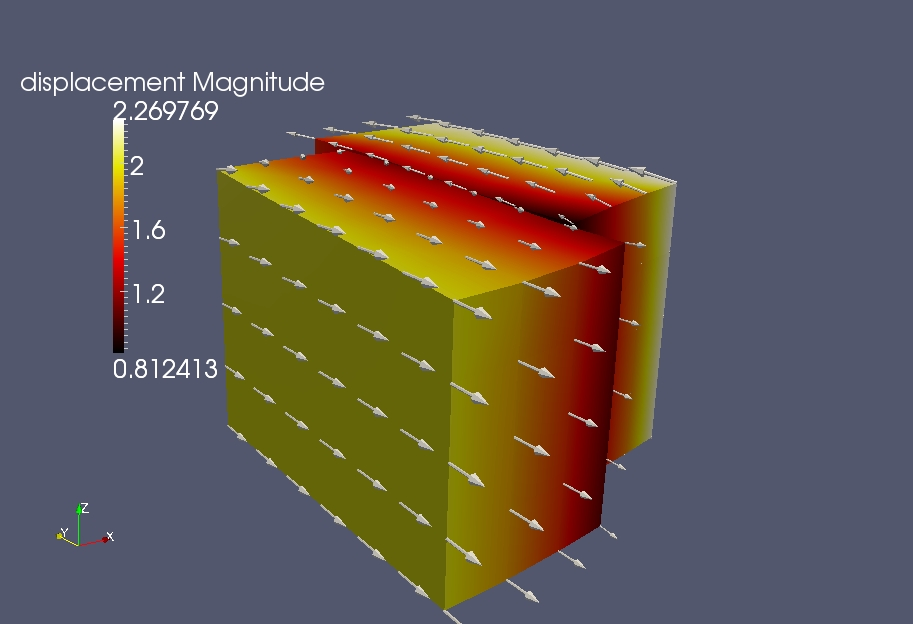
\includegraphics[width=10cm]{tutorials/3dhex8/figs/step13-displ-t200}
\par\end{centering}

\caption{Displacement field for example step13 at t = 200 years visualized
using ParaView. The mesh has been distorted by the computed displacements
(magnified by 500), and the vectors show the computed displacements.\label{fig:step13-displ-t200}}
\end{figure}



\subsubsection{Step14 - Rate-and-State Friction with Quasi-Static Dirichlet Boundary
Conditions}

In step14 we use a rate-and-state friction model with an ageing law
instead of a slip-weakening friction model. Slip begins to occur at
about t = 45 years, and continues in each subsequent time step. We
again use a constant time step size of 5 years and apply the same
intial displacement and velocity boundary conditions.

We first define the friction model for the simulation:
\begin{lyxcode}
{[}pylithapp.timedependent.interfaces.fault{]}

\#~Use~the~rate-and-state~aging~friction~model.

friction~=~pylith.friction.RateStateAgeing
\end{lyxcode}
The rate-and-state constitutive model requires a vreference coefficient
of friction, a vreference slip rate, a slip weakening parameter, an
a-value, a b-value, and a cohesion (see \vref{sec:fault:constitutive:models}):
\begin{lyxcode}
{\small{}{[}pylithapp.timedependent.interfaces.fault{]}}{\small \par}

{\small{}\#~Set~rate-and-state~parameters~using~a~UniformDB.~Set~the~parameters~as}{\small \par}

{\small{}\#~follows:}{\small \par}

{\small{}\#~vreference~coefficient~of~friction:~0.6}{\small \par}

{\small{}\#~vreference~slip~rate:~1.0e-06~m/s}{\small \par}

{\small{}\#~slip-weakening~parameter:~0.037~m}{\small \par}

{\small{}\#~a:~0.0125}{\small \par}

{\small{}\#~b:~0.0172}{\small \par}

{\small{}\#~cohesion:~0~Pa}{\small \par}

{\small{}friction.db\_properties~=~spatialdata.spatialdb.UniformDB}{\small \par}

{\small{}friction.db\_properties.label~=~Rate~State~Ageing}{\small \par}

{\small{}friction.db\_properties.values~=~{[}vreference-friction-coefficient,vreference-slip-rate,}~\\
{\small{}characteristic-slip-distance,constitutive-parameter-a,constitutive-parameter-b,cohesion{]}}{\small \par}

{\small{}friction.db\_properties.data~=~{[}0.6,1.0e-6{*}m/s,0.0370{*}m,0.0125,0.0172,0.0{*}Pa{]}}{\small \par}
\end{lyxcode}
For this model, we also want to set the initial value of the state
variable:
\begin{lyxcode}
{[}pylithapp.timedependent.interfaces.fault{]}

\#~Set~spatial~database~for~the~initial~value~of~the~state~variable.

friction.db\_initial\_state~=~spatialdata.spatialdb.UniformDB

friction.db\_initial\_state.label~=~Rate~State~Ageing~State

friction.db\_initial\_state.values~=~{[}state-variable{]}

friction.db\_initial\_state.data~=~{[}92.7{*}s{]}
\end{lyxcode}
When we have run the simulation, the output VTK files will be contained
in \texttt{examples/3d/hex8/output} (all with a pvrefix of \texttt{step14}).
Results using ParaView are shown in Figure \vref{fig:step14-displ-t200}.

\begin{figure}
\begin{centering}
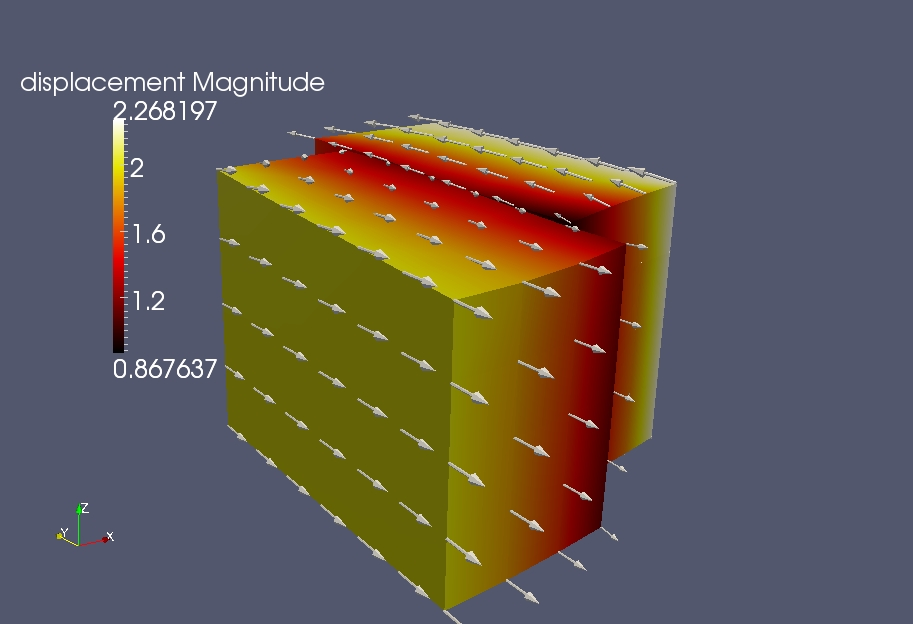
\includegraphics[width=10cm]{tutorials/3dhex8/figs/step14-displ-t200}
\par\end{centering}

\caption{Displacement field for example step14 at t = 200 years visualized
using ParaView. The mesh has been distorted by the computed displacements
(magnified by 500), and the vectors show the computed displacements.\label{fig:step14-displ-t200}}
\end{figure}


\subsection{Gravitational Body Force Examples}
\label{sec:example:3dhex8:gravity}

PyLith features discussed in this example:
\begin{itemize}
\item Gravitational body forces
\item Initial stresses
\item Finite strain
\item Generalized Maxwell linear viscoelastic material
\end{itemize}

\subsubsection{Overview}

This set of examples describes a set of problems for PyLith involving
gravitational body forces. All of the examples are quasi-static and
run for a time period of 200 years. These examples also demonstrate
the use of a generalized Maxwell viscoelastic material, which is used
for the lower crust in all examples. The final example (step17)
demonstrates the usage of a finite strain formulation, which
automatically invokes the nonlinear solver. All of the examples are
contained in the directory \filename{examples/3d/hex8}, and the
corresponding \filename{.cfg} files are \filename{step15.cfg},
\filename{step16.cfg}, and \filename{step17.cfg}.  Each example may be
run as follows:
\begin{shell}
$ pylith stepXX.cfg
\end{shell}
This will cause PyLith to read the default parameters in
\filename{pylithapp.cfg}, and then override or augment them with the
additional parameters in the \filename{stepXX.cfg} file. Each
\filename{.cfg} file is extensively documented, to provide detailed
information on the various parameters.


\subsubsection{Step15 - Gravitational Body Forces}

The \filename{step15.cfg} file defines a problem with extremely simple
Dirichlet boundary conditions. On the positive and negative x-faces,
the positive and negative y-faces, and the negative z-face, the
displacements normal to the face are set to zero. Because all of the
materials in the example have the same density, the elastic solution
for loading via gravitational body forces is
\begin{equation}
\sigma_{zz}=\rho gh;\:\sigma_{xx}=\sigma_{yy}=\frac{\nu\rho gh}{1-\nu}\:.\label{eq:1-1}
\end{equation}

We set the gravity field, which by default has values of 9.80655
$\unitfrac{m}{s^{2}}$ for acceleration and $\left[0,0,-1\right]$
for direction and time stepping implementation:
\begin{cfg}
<h>[pylithapp.timedependent]</h>
<f>gravity_field</f> = spatialdata.spatialdb.GravityField ; Set gravity field

<h>[pylithapp.timedependent.implicit]</h>
# Change time stepping algorithm from uniform time step, to adaptive
# time stepping.
<f>time_step</f> = pylith.problems.TimeStepAdapt

# Change the total simulation time to 200 years, and set the maximum time
# step size to 10 years.
<h>[pylithapp.timedependent.implicit.time_step]</h>
<p>total_time</p> = 200.0*year
<p>max_dt</p> = 10.0*year
<p>stability_factor</p> = 1.0 ; use time step equal to stable value from materials
\end{cfg}

We use a generalized Maxwell model for the lower crust (see Section
\vref{sec:materials:formulation:generalized:Maxwell}), and use a \object{SimpleDB} to
provide the properties. We also request the relevant properties and
state variables for output:
\begin{cfg}
# Change material type of lower crust to generalized Maxwell viscoelastic.
<h>[pylithapp.timedependent]</h>
<f>materials.lower_crust</f> = pylith.materials.GenMaxwellIsotropic3D
# Provide a spatial database from which to obtain property values.
# Since there are additional properties and state variables for the
# generalized Maxwell model, we explicitly request that they be output.
# Properties are named in cell\_info\_fields and state variables are named in
# cell\_data\_fields.
<h>[pylithapp.timedependent.materials.lower_crust]</h>
<p>db_properties.iohandler.filename</p> = spatialdb/mat\_genmaxwell.spatialdb
<p>output.cell_info_fields</p> = [density, mu, lambda, shear_ratio, maxwell_time]
<p>output.cell_data_fields</p> = [total_strain, stress, viscous_strain_1, viscous_strain_2, \\
  viscous_strain_3]
\end{cfg}
The boundary conditions for this example are trivial, so we are able
to use the default \object{ZeroDispDB} for all faces. When we have
run the simulation, the output VTK files will be contained in \filename{examples/3d/hex8/output}
(all with a prefix of \filename{step15}). Results using ParaView are
shown in Figure \vref{fig:example:3dhex8:step15:displacement}.

\begin{figure}
  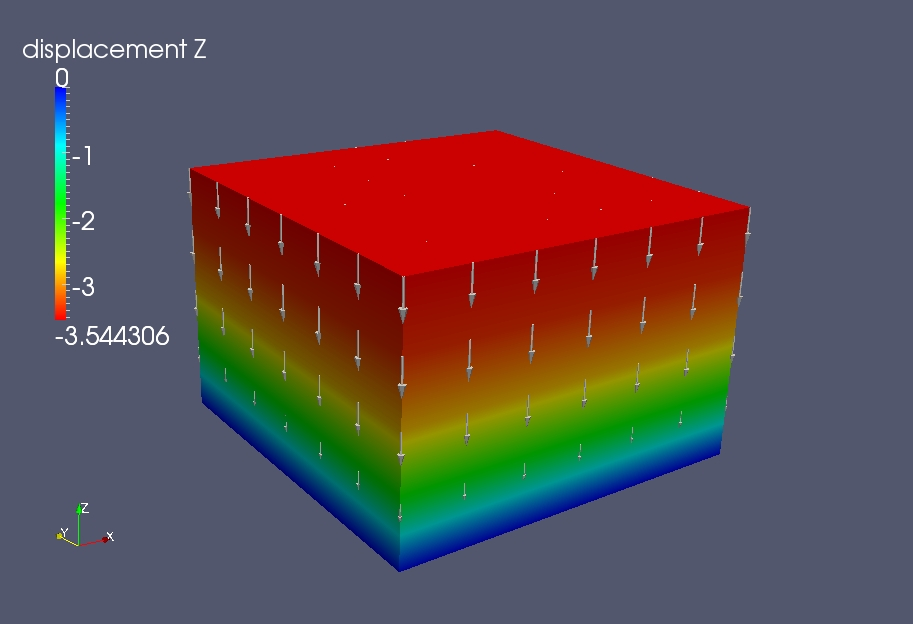
\includegraphics[width=10cm]{examples/figs/3dhex8_step15-displ-t200}
  \caption{Displacement field for example step15 at t = 200 years visualized
    using ParaView. The z-component of the displacement field is shown
    with the color contours, and the vectors show the computed displacements.}
  \label{fig:example:3dhex8:step15:displacement}
\end{figure}


\subsubsection{Step16 - Gravitational Body Forces with Initial Stresses}

The \filename{step16.cfg} file defines a problem that is identical to
example step15, except that initial stresses are used to prevent the
initial large displacements due to 'turning on' gravity. Since all
normal stress components are given an initial stress of $\rho gh$,
the initial stress state is lithostatic, which is an appropriate condition
for many tectonic problems in the absence of tectonic stresses (e.g.,
McGarr \cite{McGarr:1988}). When compared to example step15, this
example should maintain a lithostatic state of stress for the entire
simulation, and displacements should remain essentially zero.

We set the gravity field, as in example step15, and we again use adaptive
time stepping with a generalized Maxwell rheology for the lower crust.
We provide values for the initial stress for both the upper and lower
crust. Since the materials have the same density, we are able to use
the same \object{SimpleDB} with a linear variation for both (see file
\filename{examples/3d/hex8/spatialdb/initial\_stress.spatialdb}):
\begin{cfg}
# We must specify initial stresses for each material.
# We provide a filename for the spatial database that gives the stresses,
# and we change the query_type from the default 'nearest' to 'linear'.
<h>[pylithapp.timedependent.materials.upper_crust]</h>
<f>db_initial_stress</f> = spatialdata.spatialdb.SimpleDB
<p>db_initial_stress.iohandler.filename</p> = spatialdb/initial_stress.spatialdb
<p>db_initial_stress.query_type</p> = linear

<h>[pylithapp.timedependent.materials.lower_crust]</h>
<f>db_initial_stress</f> = spatialdata.spatialdb.SimpleDB
<p>db_initial_stress.iohandler.filename</p> = spatialdb/initial_stress.spatialdb
<p>db_initial_stress.query_type</p> = linear
\end{cfg}
Note that we use a \texttt{linear} \property{query\_type} rather than
the default type of \texttt{nearest}, so that a linear interpolation
is performed along the z-direction. When we have run the simulation,
the output VTK files will be contained in \filename{examples/3d/hex8/output}
(all with a prefix of \filename{step16}). Results using ParaView are
shown in Figure \vref{fig:example:3dhex8:step16:stress}.

\begin{figure}
  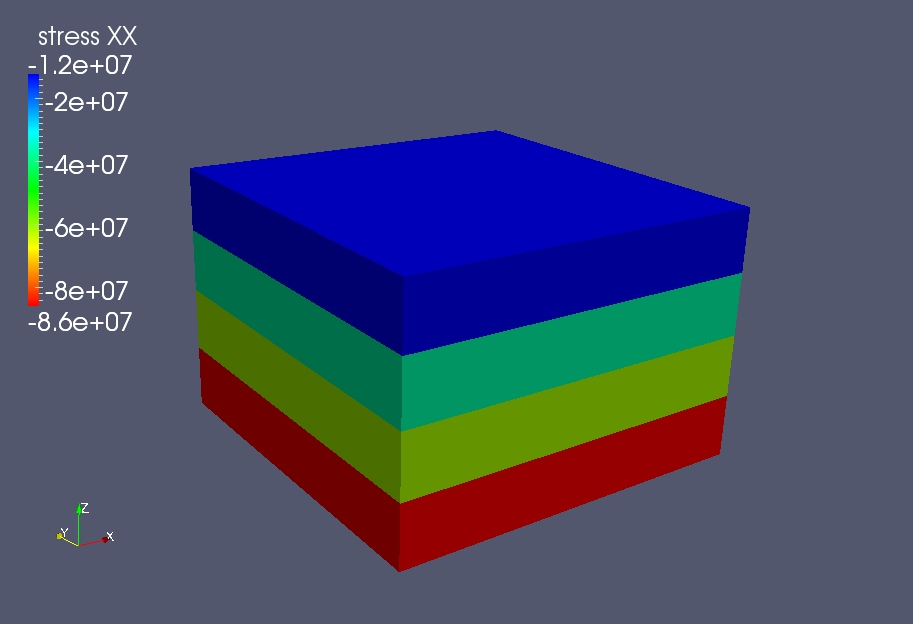
\includegraphics[width=10cm]{examples/figs/3dhex8_step16-stress_xx-t200}
  \caption{Stress field (xx-component) for example step16 at t = 200 years visualized
    using ParaView. Note that for this example, Stress\_xx = Stress\_yy
    = Stress\_zz, and there is no vertical displacement throughout the
    simulation. Also note that the stresses appear as four layers since
    we have used \object{CellFilterAvg} for material output.}
  \label{fig:example:3dhex8:step16:stress}
\end{figure}


\subsubsection{Step17 - Gravitational Body Forces with Small Strain}

The \filename{step17.cfg} file defines a problem that is identical to
example step15, except that we now use a small strain formulation
(see Section \vref{sec:small:strain:formulation}). All of the problems
up to this point have assumed infinitesimal strain, meaning that the
change in shape of the domain during deformation is not taken into
account. In many problems it is important to consider the change in
shape of the domain. This is particularly important in many problems
involving gravitational body forces, since a change in shape of the
domain results in a different stress field. By examining the stress
and deformation fields for this example in comparison with those of
example step15, we can see what effect the infinitesimal strain approximation
has on our solution.

We set the gravity field, as in example step15 and again use adaptive
time stepping withs a generalized Maxwell rheology for the lower crust.
The only change is that we change the problem formulation from the
default \object{Implicit} to \object{ImplicitLgDeform}. Since the
large deformation formulation is nonlinear, PyLith automatically switches
the solver from the default \object{SolverLinear} to \object{SolverNonlinear}.
It is thus only necessary to change the formulation:
\begin{cfg}
<h>[pylithapp.timedependent]</h>
# Set the formulation for finite strain. The default solver will
# automatically be switched to the nonlinear solver.
<f>formulation</f> = pylith.problems.ImplicitLgDeform
\end{cfg}
When we have run the simulation, the output VTK files will be contained
in \filename{examples/3d/hex8/output} (all with a prefix of \filename{step17}).
Results using ParaView are shown in Figure \vref{fig:example:3dhex8:step17:displacement}.

\begin{figure}
  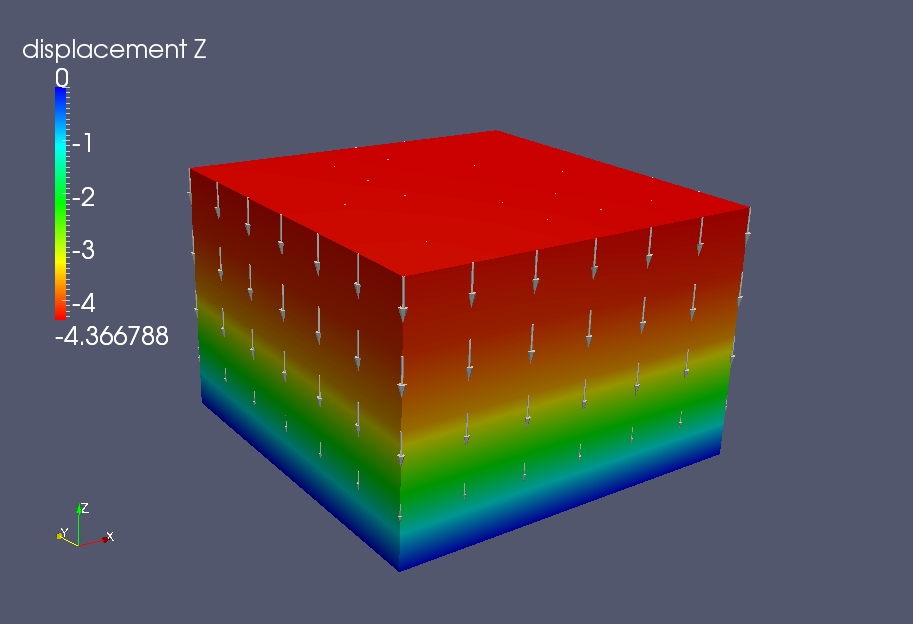
\includegraphics[width=10cm]{examples/figs/3dhex8_step17-displ-t200}
  \caption{Displacement field for example step17 at t = 200 years visualized
    using ParaView. The z-component of the displacement field is shown
    with the color contours, and the vectors show the computed displacements.
    Note the larger displacements compared with example step15.}
  \label{fig:example:3dhex8:step17:displacement}
\end{figure}


\subsection{Surface Load Traction Examples}
\label{sec:example:3dhex8:surfload}

PyLith features discussed in this example:
\begin{itemize}
\item Time-dependent Neumann (traction) boundary conditions
\item Dirichlet boundary conditions
\item Elastic material
\item Output of solution at user-defined locations
\end{itemize}

\subsubsection{Overview}

This set of examples describes a set of problems for PyLith involving
surface loading with a Neumann (traction) applied to the ground surface.
The first example demonstrates the use of a surface load in a static
problem, and the second example demonstates how to apply a cyclic
load in a quasi-static problem. The second problem also includes output
of the solution at user-defined locations. All of the examples are
contained in the directory \filename{examples/3d/hex8}, and the corresponding
\filename{cfg} files are \filename{step18.cfg} and \filename{step19.cfg}.
Each example may be run as follows:
\begin{shell}
$ pylith stepXX.cfg
\end{shell}
This will cause PyLith to read the default parameters in \filename{pylithapp.cfg},
and then override or augment them with the additional parameters in
the \filename{stepXX.cfg} file. Each \filename{cfg} file is extensively
documented, to provide detailed information on the various parameters.


\subsubsection{Step18 - Static Surface Load}

The \filename{step18.cfg} file defines a problem with a spatially varying
axial surface load applied to the top surface with Dirichlet (roller)
boundary conditions on the lateral and bottom surfaces. We first set
the array of boundary conditions with one for each surface of the
domain. As in the other examples, we also setup output for the ground
surface.

For the Dirichlet boundary conditions we fix the degree of freedom
associated with motion normal to the boundary while leaving the other
degrees of freedom free. We do not explicitly specify the use of a
Dirichlet boundary condition because it is the default. Similarly,
the ZeroDispDB is the default spatial database for the displacements
in a Dirichlet boundary condition, so all we need to specify is the
degree of freedom that is constrained, the name of the nodeset from
CUBIT, and a label used in diagnostic output. For the Dirichlet boundary
condition on the +x surface we have:
\begin{cfg}
<h>[pylithapp.timedependent.bc.x_pos]</h>
<p>label</p> = face_xpos
<p>bc_dof</p> = [0]

<p>db_initial.label</p> = Dirichlet BC on +x
\end{cfg}
On the top surface we apply a Neumann boundary condition for the surface
load, so we first set the boundary condition type and then specify
the nodeset in CUBIT associated with this surface. For the static
surface load, we use a spatial database for the initial value and
linear interpolation. We integrate the surface tractions over the
boundary, so we also specify the numerical integration scheme to use.
Finally, we specify a vector for the up direction because the tractions
are applied to a horizontal surface, resulting in ambiguous shear
directions for our default orientation convention.
\begin{cfg}
<h>[pylithapp.timedependent.bc]</h>
<f>z_pos</f> = pylith.bc.Neumann

<h>[pylithapp.timedependent.bc.z_pos]</h>
<p>label</p> = face_zpos

<f>db_initial</f> = spatialdata.spatialdb.SimpleDB
<p>db_initial.label</p> = Neumann BC on +z
<p>db_initial.iohandler.filename</p> = spatialdb/tractions\_axial\_pressure.spatialdb
<p>db_initial.query_type</p> = linear ; Use linear interpolation.

# Diagnostic output
<p>output.cell_info_fields</p> = [initial-value]
<p>output.writer.filename</p> = output/step18-traction.vtk
<f>output.cell_filter</f> = pylith.meshio.CellFilterAvg

# We must specify quadrature information for the cell faces.
<f>quadrature.cell</f> = pylith.feassemble.FIATLagrange
<p>quadrature.cell.dimension</p> = 2
<p>quadrature.cell.quad_order</p> = 2 \\

# Because normal for +z surface is {[}0,0,1{]}, the horizontal and
# vertical shear directions are ambiguous. We provide a ``fake'' up
# direction of [0,1,0] so that the horizontal shear direction (cross
# product of ``up'' and normal is [1,0,0] and the vertical shear
# direction (cross product of normal and horizontal) is [0,1,0].
<p>up_dir</p> = [0,1,0]
\end{cfg}
When we have run the simulation, the output VTK files will be contained
in \filename{examples/3d/hex8/output} (all with a prefix of \filename{step18}).
Results using ParaView are shown in Figure \vref{fig:example:3dhex8:step18:displacement}.

\begin{figure}
  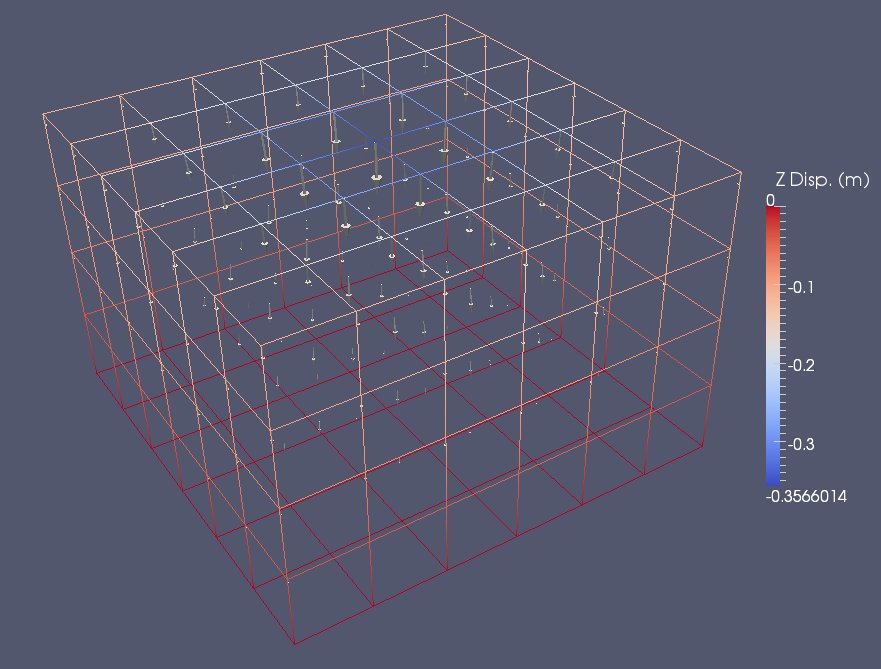
\includegraphics[width=10cm]{examples/figs/3dhex8_step18-displ}
  \caption{Displacement field for example step18 visualized using ParaView. The
    vectors show the displacement field while the colors in the wireframe
    correspond to the z-component of the displacement field.}
  \label{fig:example:3dhex8:step18:displacement}
\end{figure}


\subsubsection{Step19 - Time-Dependent Surface Load}

The \filename{step19.cfg} file defines a problem that is identical to
example step18, except that we vary the amplitude of the surface load
as a function of time. We use a temporal database (analogous to our
spatial databases for specifying spatial variations) to prescribe
a piecewise linear variation of the amplitude with time as given in
the file \filename{spatialdb/loadcycle.timedb}. The amplitude begins
at zero, progresses to 1.0, then 1.5, before decreasing in a symmetric
fashion. The temporal database can use variable time steps to prescribe
arbitrary time histories. 

Rather than specify a spatial database for the initial value of the
Neumann boundary condition corresponding to the surface load, we specify
a spatial database for the change in value and the temporal database:
\begin{cfg}
<h>[pylithapp.timedependent.bc.z_pos]</h>
<p>label</p> = face_zpos

<f>db_change</f> = spatialdata.spatialdb.SimpleDB
<p>db_change.label</p> = Amplitude of Neumann BC on +z
<p>db_change.iohandler.filename</p> = spatialdb/tractions_axial_pressure.spatialdb
<p>db_change.query_type</p> = linear ; Use linear interpolation

<f>th_change</f> = spatialdata.spatialdb.TimeHistory
<p>th_change.label</p> = Time history for Neumann BC on +z
<p>th_change.filename</p> = spatialdb/loadcycle.timedb
\end{cfg}
When we have run the simulation, the output VTK files will be contained
in \filename{examples/3d/hex8/output} (all with a prefix of \filename{step19}).
Results using ParaView are shown in Figure \vref{fig:example:3dhex8:step19:stress}.
We also output the solution at user-defined locations, which are given
in the file \filename{output\_points.txt.} See Section \vref{sec:output:points}
for a discussion of the output parameters. This type of output is
designed for comparison against observations and inversions and output
via HDF5 files (see Section \vref{sub:HDF5/Xdmf-Output}).

\begin{figure}
  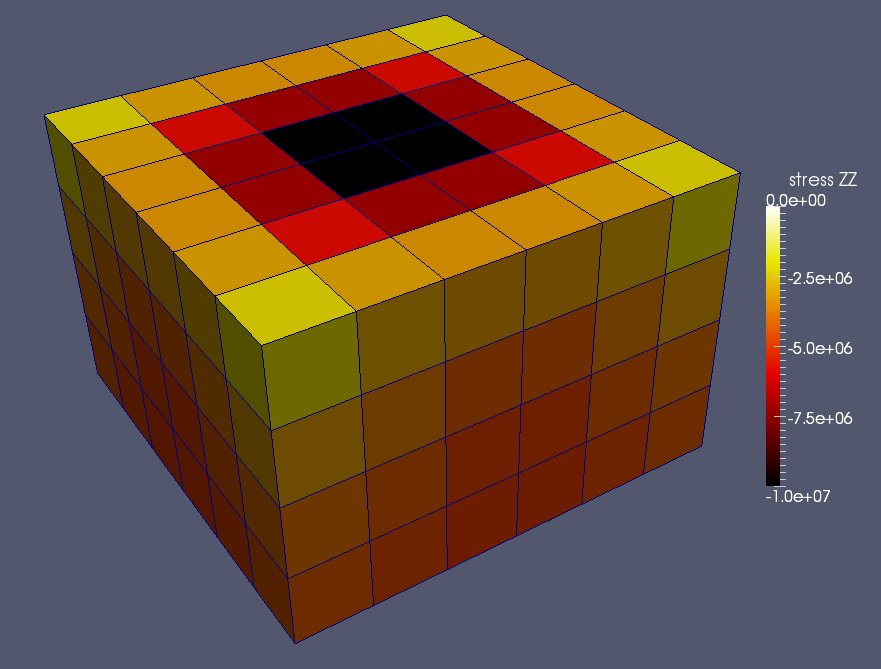
\includegraphics[width=10cm]{examples/figs/3dhex8_step19-stress_t200}
  \caption{Stress field (zz-component) for example step19 at t = 200
    years visualized using ParaView. The stresses appear as four
    layers since we have used \object{CellFilterAvg} for material
    output.}
  \label{fig:example:3dhex8:step19:stress}
\end{figure}

% End of file

\subsection{Dike Intrusion Example}
\label{sec:example:3dhex8:dike}

PyLith features discussed in this example:
\begin{itemize}
\item Fault opening via prescribed tractions to mimic a dike instrusion
\item Dirichlet boundary conditions
\item Elastic material
\item VTK output
\end{itemize}

\subsubsection{Overview}

This set of examples describes a problem where prescribed tensile
tractions are imposed on a fault to mimic a dike intrusion. The example
is contained in the directory \filename{examples/3d/hex8}, and the corresponding
\filename{cfg} file is \filename{step20.cfg}. The example may be run
as follows:
\begin{shell}
$ pylith step20.cfg
\end{shell}
This will cause PyLith to read the default parameters in \filename{pylithapp.cfg},
and then override or augment them with the additional parameters in
the \filename{step20.cfg} file. The \filename{cfg} file is extensively
documented, to provide detailed information on the various parameters.


\subsubsection{Step20 - Static Dike Intrusion}

The \filename{step20.cfg} file defines a problem with spatially varying
tensile normal tractions on the fault surface associated with a fluid
intrusion. The lateral sides and bottom of the domain are fixed using
Dirichlet (roller) boundary conditions. As in the other examples,
we also setup output for the ground surface.

We use the FaultCohesiveDyn object to impose tractions on the fault
surface. We must include a fault constitutive model so we choose static
friction with a coefficient of friction of 0.1. The coefficient of
friction is irrelevant for the center of the fault where we impose
uniform tensile tractions (10 MPa) and the fault opens, but it facilitates
clamping the edges of the fault via compressive normal tractions (-100
MPa). Note that we must set the property \property{open\_free\_surface}
to False in order for the tractions to be imposed when the fault is
open; the default behavior for fault opening is a free surface (the
two sides of the fault are completely uncoupled). The most important
fault parameters for prescribing the tensile fault tractions are
\begin{cfg}
<h>[pylithapp.timedependent.interfaces.fault]</h>
<p>open_free_surface</p> = False
<f>traction_perturbation</f> = pylith.faults.TractPerturbation

<h>[pylithapp.timedependent.interfaces.fault.traction_perturbation]</h>
<f>db_initial</f> = spatialdata.spatialdb.SimpleDB
<p>db_initial.label</p> = Initial fault tractions
<p>db_initial.iohandler.filename</p> = spatialdb/tractions_opening.spatialdb
<p>db_initial.query_type</p> = nearest 
\end{cfg}
When we have run the simulation, the output VTK files will be contained
in \filename{examples/3d/hex8/output} (all with a prefix of \filename{step20}).
Results using ParaView are shown in Figure \vref{fig:example:3dhex8:step20:displacement}.

\begin{figure}
  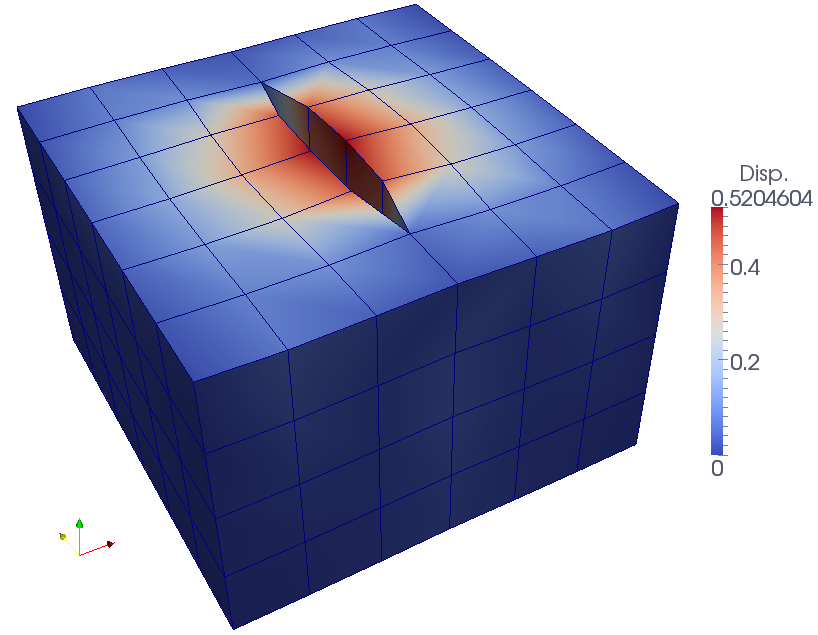
\includegraphics[width=10cm]{examples/figs/3dhex8_step20_disp}
  \caption{Displacement magnitude for example step20 visualized using ParaView.}
  \label{fig:example:3dhex8:step20:displacement}
\end{figure}


% End of file

\subsection{Green's Functions Generation Example}
\label{sec:example:3dhex8:greensfns}

PyLith features discussed in this example:
\begin{itemize}
\item Generation of Green's functions from a fault
\item Kinematic fault impulses
\item Running a different problem type
\item Dirichlet boundary conditions
\item Elastic material
\item HDF5 output
\item Interpolated point output
\end{itemize}

\subsubsection{Overview}

This example describes a problem where we generate a set of Green's
functions that could be used in an inversion. The example is contained
in the directory \filename{examples/3d/hex8}, and the corresponding
\filename{.cfg} file is \filename{step21.cfg}. The example may be run
as follows:
\begin{shell}
$ pylith step21.cfg --problem=pylith.problems.GreensFns
\end{shell}
This will cause PyLith to read the default parameters in
\filename{pylithapp.cfg} and \filename{greensfns.cfg}, and then
override or augment them with the additional parameters in the
\filename{step21.cfg} file. The \filename{.cfg} files are extensively
documented, to provide detailed information on the various parameters.


\subsubsection{Step21 - Green's Function Generation}

This problem makes use of two \filename{.cfg} files that are read by
default -- \filename{pylithapp.cfg} and \filename{greensfns.cfg}. The
\filename{greensfns.cfg} file is read automatically because we have
changed the problem type to \object{GreensFns} (as opposed to the
default \object{TimeDependent} problem type). The facility name then
becomes \facility{greensfns}, and PyLith will therefore search for a
\filename{.cfg} file matching the name of the facility. The
\filename{greensfns.cfg} file contains settings that are specific to
the \object{GreensFns} problem type:
\begin{cfg}
<h>[greensfns]</h>
<p>fault_id</p> = 10

<h>[greensfns.interfaces]</h>
<f>fault</f> = pylith.faults.FaultCohesiveImpulses

<h>[greensfns.interfaces.fault]</h>
<p>impulse_dof</p> = [0, 1]

<p>db_impulse_amplitude.label</p> = Amplitude of slip impulses
<p>db_impulse_amplitude.iohandler.filename</p> = spatialdb/impulse_amplitude.spatialdb
<p>db_impulse_amplitude.query_type</p> = nearest 
\end{cfg}
We specify the \property{fault\_id}, which is required by the \object{GreensFns}
problem type (it is the same as the ID used when generating the mesh).
We also change the fault type to \object{FaultCohesiveImpulses}, which
allows us to apply a single impulse of slip for each impulse with
a nonzero slip value in the corresponding spatial database file
(\filename{spatialdb/impulse\_amplitude.spatialdb}). We indicate that
we would like to apply slip impulses in both the left-lateral (\property{impulse\_dof}
= 0) and updip (\property{impulse\_dof} = 1) directions, and we use
nearest-neighbor interpolation to determine the amount of applied
slip. Note that in the \filename{spatialdb/impulse\_amplitude.spatialdb}
file we specify negative slip, thus reversing the sense of applied
slip for both slip directions. Note that we also put a margin of zeros
around the edge of the fault, which prevents impulses from being applied
along this boundary.

The \filename{step21.cfg} file defines the remainder of the parameters
for this problem. The boundary conditions and fault information are
provided as for previous examples. Rather than computing the solution
over the ground surface, we choose to provide output at a set of points.
PyLith provides the ability to interpolate displacements to a specified
set of points, which would generally be necessary when generating
Green's functions:
\begin{cfg}
<h>[pylithapp.problem.formulation]</h>
<f>output</f> = [domain, points]
<f>output.points</f> = pylith.meshio.OutputSolnPoints

<h>[pylithapp.problem.formulation.output.points]</h>
<f>writer</f> = pylith.meshio.DataWriterHDF5
<p>writer.filename</p> = output/step21-points.h5
<p>reader.filename</p> = greensfns_points.txt
<p>coordsys.space_dim</p> = 3
<p>coordsys.units</p> = m
\end{cfg}
We first define \object{OutputSolnPoints} as the output manager for
points output. We use HDF5 output for all of the Green's function
output, as it will generally be more efficient (faster I/O, smaller
file sizes). We must provide a set of points for point output. The
file \filename{greensfns\_points.txt} contains a set of (x,y,z) coordinates.
We must also provide the spatial dimension of the coordinates as well
as the units used. Note that we do not output any info or data fields
for state variable output, as this would otherwise create a large
amount of output for each applied slip impulse. When we have run the
simulation, the output HDF5 files will be contained in \filename{examples/3d/hex8/output}
(all with a prefix of \filename{step21}). In Figure \vref{fig:example:3dhex8:step21:impluse}
we show an impulse of left-lateral slip applied on the fault and the
resulting response at the specified set of points. The time corresponds
to the impulse number in multiples of the specified time step size.

\begin{figure}
  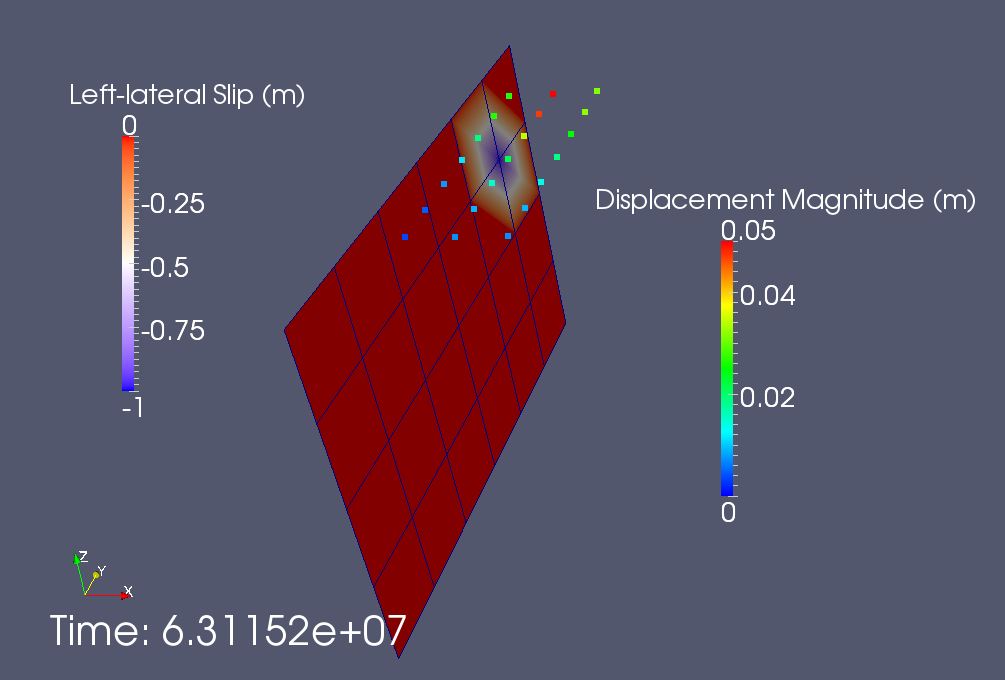
\includegraphics[width=10cm]{examples/figs/3dhex8_step21_impulse_resp}
  \caption{A slip impulse and the resulting point displacement
    responses visualized using ParaView. }
  \label{fig:example:3dhex8:step21:impluse}
\end{figure}


% End of file


% End of file
\section{Tutorial for Slip on a Subduction Zone}
\label{sec:example:subduction}

PyLith features discussed in this tutorial:
\begin{itemize}
\item Static solution
\item Quasi-static solution
\item CUBIT mesh generation
\item Nonplanar geometry
\item Variable mesh resolution
\item APREPRO programming language
\item Linear triangular cells
\item HDF5 output
\item Dirichlet displacement and velocity boundary conditions
\item ZeroDispDB spatial database
\item SimpleDB spatial database
\item UniformDB spatial database
\item Multiple materials
\item Nonlinear solver
\item Plane strain linearly elastic material
\item Plane Maxwell linear viscoelastic material
\item Prescribed slip
\item Static fault rupture
\item Multiple faults
\item Spatially variable coseismic slip
\item Spatially variable aseismic creep
\item Afterslip via fault friction
\item Static fault rupture
\item Static friction
\end{itemize}
All of the files necessary to run the examples are contained in the
directory \filename{examples/2d/subduction.}


\subsection{Overview}

This tutorial examines quasi-static interseismic and coseismic
deformation in 2D for a subduction zone (see Figure
\vref{fig:tutorial:subduction:overview}).  It is based on the 2011
M9.0 Tohoku earthquake off the east coast of Japan. Figure
\vref{fig:tutorial:subduction:steps} shows the three steps of
increasing complexity. Step 1 focuses on the coseismic slip, Step 2
focuses on interseismic deformation, and Step 3 combines the two into
a pseudo-earthquake cycle deformation simulation. Step 4 focuses on
using the change in tractions from Step 1 to construct a simulation
with afterslip controlled by frictional sliding.

\begin{figure}
  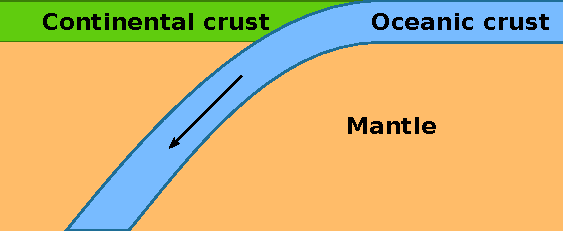
\includegraphics{examples/figs/subduction_cartoon_general}
  \caption{Cartoon of subduction zone example.}
  \label{fig:tutorial:subduction:overview}
\end{figure}

\begin{figure}
  \begin{tabular}{ccc}
    Step 1 & Step 2 & Step 3 \\
    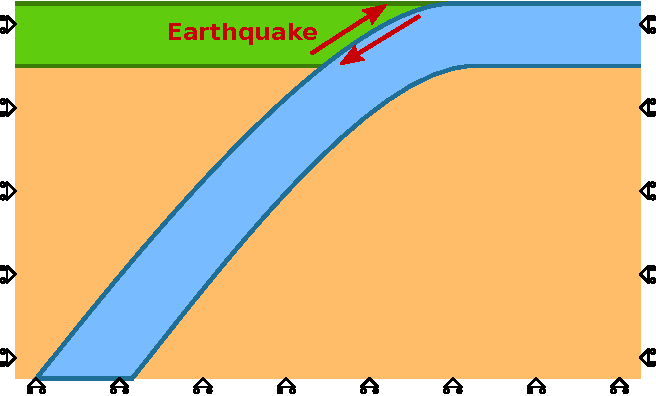
\includegraphics[width=2in]{examples/figs/subduction_step01} &
    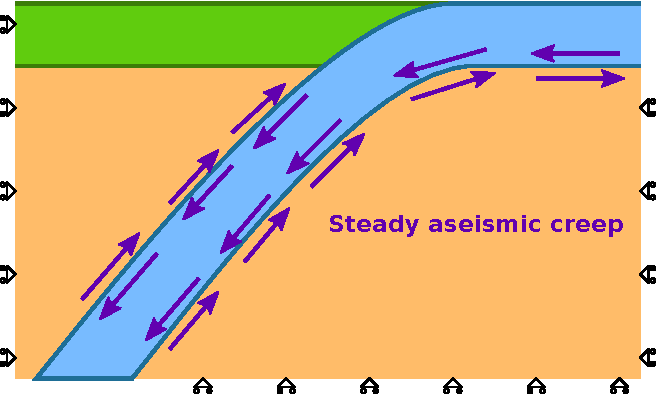
\includegraphics[width=2in]{examples/figs/subduction_step02} & 
    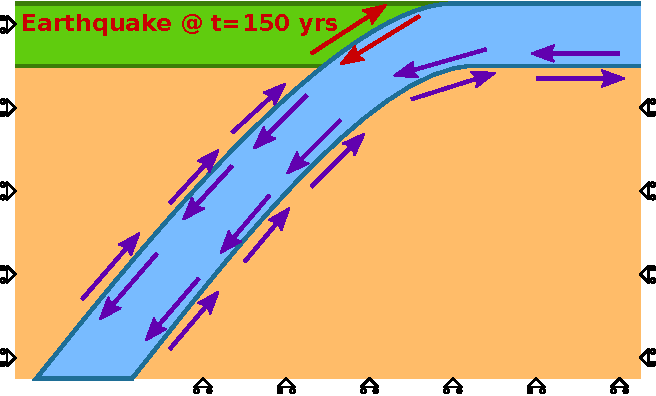
\includegraphics[width=2in]{examples/figs/subduction_step03} \\
  \end{tabular}
  \caption{Diagram of fault slip and boundary conditions for each step in the
    subduction zone tutorial.}
  \label{fig:tutorial:subduction:steps}
\end{figure}


\subsection{Mesh Description}

We construct the mesh in CUBIT by constructing the geometry, prescribing
the discretization, running the mesher, and then grouping cells and
vertices for boundary conditions and materials. We use the APREPRO
programming language within the journal files to enable use of units
and to set variables for values used many times. An appendix in the
CUBIT documentation discusses the features available with APREPRO
in CUBIT. The CUBIT commands are in three separate journal files.
The main driver is in the journal file \filename{mesh\_tri3.jou}. It
calls the journal file \filename{geometry.jou} to construct the geometry
and \filename{createbc.jou} to set up the groups associated with boundary
conditions and materials. The journal files are documented and describe
the various steps outlined below.
\begin{enumerate}
\item Create the geometry defining the domain.
  \begin{enumerate}
  \item Create points.
  \item Connect points into spline curves.
  \item Split curves to separate them into sections bounding surfaces. 
  \item Connect curves into surfaces.
  \item Stitch surfaces together.
  \end{enumerate}
\item Define meshing scheme and cell size variation.
  \begin{enumerate}
  \item Define cell size along curves near fault.
  \item Increase cell size away from fault at a geometric rate (bias).
  \end{enumerate}
\item Generate mesh.
\item Create blocks for materials and nodesets for boundary conditions.
\item Export mesh.
\end{enumerate}

\begin{figure}
  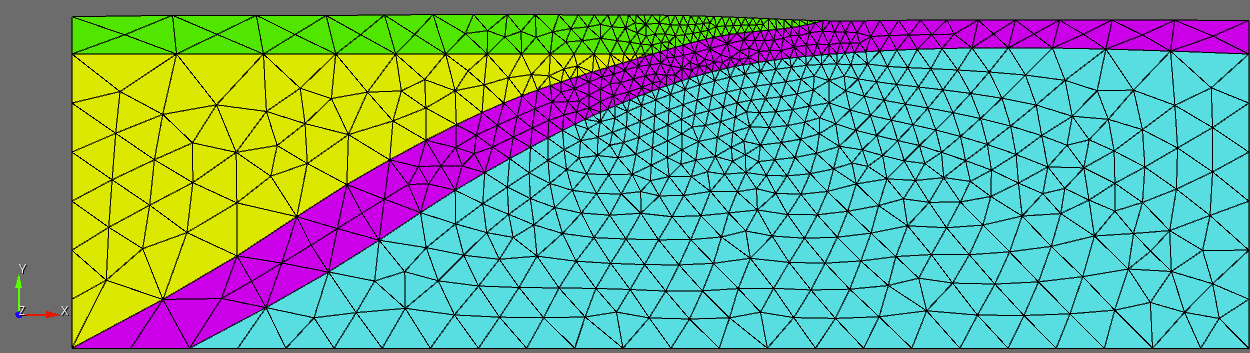
\includegraphics[width=4.5in]{examples/figs/subduction_tri3}
  \caption{Variable resolution finite-element mesh with triangular
    cells. The nominal cell size increases at a geometric rate of 1.2
    away from the region of coseismic slip.}
  \label{fig:tutorial:subduction:mesh}
\end{figure}


\subsection{Common Information}

As in the examples discussed in previous sections of these tutorials,
we place parameters common to the three steps in the \filename{pylithapp.cfg}
file so that we do not have to duplicate them for each step. The settings
contained in \filename{pylithapp.cfg} for this problem consist of:
\begin{inventory}
  \facilityitem{pylithapp.journal.info}{Settings that control the
    verbosity of the output written to stdout for the different
    components.}  \facilityitem{pylithapp.mesh\_generator}{Settings
    that control mesh importing, such as the importer type, the
    filename, and the spatial dimension of the mesh.}
  \facilityitem{pylithapp.timedependent}{Settings that control the
    problem, such as the total time, time-step size, and spatial
    dimension.}
  \facilityitem{pylithapp.timedependent.materials}{Settings that
    control the material type, specify which material IDs are to be
    associated with a particular material type, and give the name of
    the spatial database containing the physical properties for the
    material. The quadrature information is also given.}
  \facilityitem{pylithapp.problem.formulation.output}{Settings related
    output of the solution over the domain and subdomain (ground
    surface).}
  \facilityitem{pylithapp.timedependent.materials.\textit{MATERIAL}.output}{Settings
    related to output of the state variables for material
    \textit{MATERIAL}.}  \facilityitem{pylithapp.petsc}{PETSc settings
    to use for the problem, such as the preconditioner type.}
\end{inventory}
The physical properties for each material are specified in spatial
database files. For example, the elastic properties for the
continental crust are in \filename{mat\_concrust.spatialdb}. The
provided spatial database files all use just a single point to specify
uniform physical properties within each material. A good exercise is
to alter the spatial database files with the physical properties to
match PREM.


\subsection{Step 1: Coseismic Slip Simulation}

The first example problem is earthquake rupture involving coseismic
slip along the interface between the subducting slab and the continental
crust and uppermost portion of the mantle below the continental crust.
The spatial variation of slip comes from a cross-section of Gavin
Hayes' finite-source model \url{earthquake.usgs.gov/earthquakes/eqinthenews/2011/usc0001xgp/finite_fault.php}.
On the lateral and bottom boundaries of the domain, we fix the degrees
of freedom perpendicular to the boundary as shown in Figure \vref{fig:tutorial:subduction:steps}.
Parameter settings that augment those in \filename{pylithapp.cfg} are
contained in the file \filename{step01.cfg}. These settings are:
\begin{inventory}
  \facilityitem{pylithapp.timedependent.formulation.time\_step}{Adjust the total
    simulation time to 0 years (static simulation).}
  \facilityitem{pylithapp.timedependent}{Specifies the array of
    boundary conditions.}
  \facilityitem{pylithapp.timedependent.bc.\textit{BOUNDARY}}{Defines the settings
    for boundary \textit{BOUNDARY}, including which degrees of freedom
    are being constrained (x or y), the label (defined in\filename{ mesh\_tri3.exo})
    corresponding to the nodeset in CUBIT, and a label to the boundary
    condition used in any error messages.}
  \facilityitem{pylithapp.timedependent.interfaces.fault}{Specify the coseismic
    slip along the interface between the oceanic crust and continental
    crust with a small amount of slip penetrating into the upper mantle.}
  \facilityitem{pylithapp.problem.formulation.output.domain}{Gives the base filenames
    for HDF5 output (for example, \filename{step01.h5}).}
\end{inventory}
We run this example by typing
\begin{shell}
$$ pylith step01.cfg
\end{shell}
The problem will produce twelve pairs of HDF5/Xdmf files. The HDF5
files contain the data and the Xdmf files contain the metadata required
by ParaView and Visit (and possibly other visualization tools that
use Xdmf files) to access the mesh and data sets in the HDF5 files.
The files include the solution over the domain and ground surface
(two pairs of files), physical properties, stress, and strain within
each material (eight pairs of files), and fault parameters, slip,
and traction (two pairs of files). 

Figure \vref{fig:tutorial:subduction:step01}, which was created using
ParaView, displays the magnitude of the displacement field with the
deformation exaggerated by a factor of 1000. 

\begin{figure}
  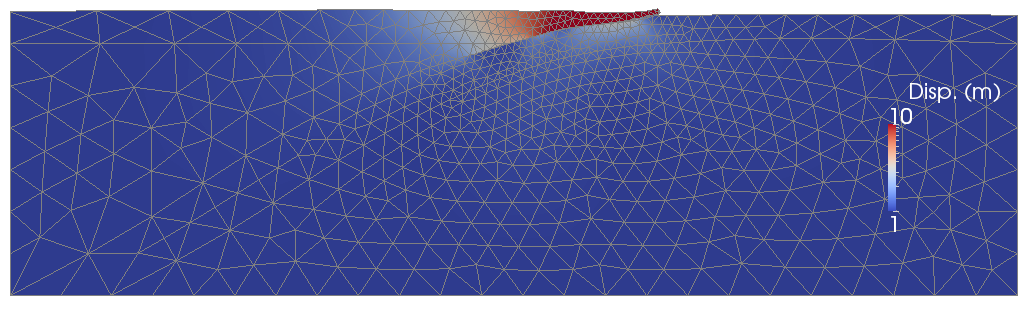
\includegraphics[width=4.5in]{examples/figs/subduction_step01_soln}
  \caption{Solution for Step 1. The colors indicate the magnitude of the displacement,
    and the deformation is exaggerated by a factor of 1000. }
  \label{fig:tutorial:subduction:step01}
\end{figure}


\subsection{Step 2: Interseismic Deformation Simulation}

In this example we simulate the interseismic deformation associated
with the oceanic crust subducting beneath the continental crust and
into the mantle. We prescribe steady aseismic slip of 8 cm/yr along
the interfaces between the oceanic crust and mantle with the interface
between the oceanic crust and continental crust locked as shown in
Figure \vref{fig:tutorial:subduction:steps}. We adjust the Dirichlet
boundary conditions on the lateral edges and bottom of the domain
by pinning only the portions of the boundaries in the mantle and continental
crust (i.e., not part of the oceanic crust). Parameter settings that
augment those in \filename{pylithapp.cfg} are contained in the file
\filename{step02.cfg}. These settings include:
\begin{inventory}
  \facilityitem{pylithapp.timedependent.formulation.time\_step}{Adjust the total
    simulation time to 100 years.}
  \facilityitem{pylithapp.timedependent}{Specifies the array of boundary conditions.}
  \facilityitem{pylithapp.timedependent.bc.\textit{BOUNDARY}}{Defines the settings
    for boundary \textit{BOUNDARY}, including which degrees of freedom
    are being constrained (x or y), the label (defined in\filename{ mesh\_tri3.exo})
    corresponding to the nodeset in CUBIT, and a label to the boundary
    condition used in any error messages.}
  \facilityitem{pylithapp.timedependent.interfaces}{Specify the steady aseismic
    slip as a constant slip rate on the fault surfaces.}
  \facilityitem{pylithapp.problem.formulation.output.domain}{Gives the base filename
    for HDF5 output (for example, \filename{step02.h5}).}
\end{inventory}
We run this example by typing
\begin{shell}
$$ pylith step02.cfg
\end{shell}
The simulation will produce pairs of HDF5/Xdmf files with separate
files for each material and fault interface. Figure
\vref{fig:tutorial:subduction:step02}, which was created using
ParaView, displays the magnitude of the displacement field with the
deformation exaggerated by a factor of 1000. Using the animation
features within ParaView or Visit you can illustrate how the
continental crust near the trench subsides during the interseismic
deformation.

\begin{figure}
  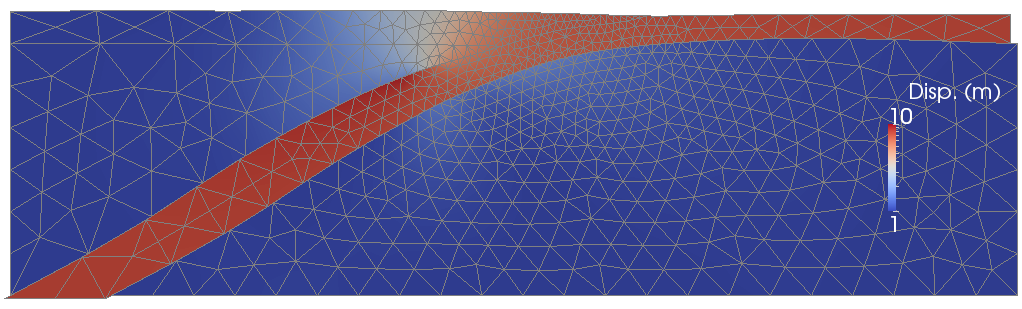
\includegraphics[width=4.5in]{examples/figs/subduction_step02_soln}
  \caption{Solution for Step 2 at 100 years. The colors indicate the
    magnitude of the displacement, and the deformation is exaggerated
    by a factor of 1000.}
  \label{fig:tutorial:subduction:step02}
\end{figure}


\subsection{Step 3: Pseudo-Earthquake Cycle Model}

This simulation combines 300 years of interseismic deformation from
Step 2 with the coseismic deformation from Step 1 applied at 150 years
to create a simple model of the earthquake cycle. Parameter settings
that augment those in \filename{pylithapp.cfg} are contained in the
file \filename{step03.cfg}. These settings include:
\begin{inventory}
  \facilityitem{pylithapp.timedependent.formulation.time\_step}{Adjust the total
    simulation time to 300 years.}
  \facilityitem{pylithapp.timedependent}{Specifies the array of boundary conditions.}
  \facilityitem{pylithapp.timedependent.bc.\textit{BOUNDARY}}{The Dirichlet boundary
    conditions match those in Step 2.}
  \facilityitem{pylithapp.timedependent.interfaces}{On the interface between the
    subducting oceanic crust and the mantle, we prescribe the same steady,
    aseismic slip as that in Step 2. On the interface along the top of
    the subducting oceanic crust and the continental crust and mantle
    we create two earthquake ruptures, The first rupture applies the coseismic
    slip form Step 1 at 150 years, while the second rupture prescribes
    the same steady, aseismic slip as in Step 2.}
  \facilityitem{pylithapp.problem.formulation.output.domain}{Gives the base filename
    for HDF5 output (for example, \filename{step03.h5}).}
\end{inventory}
We run this example by typing
\begin{shell}
$$ pylith step03.cfg
\end{shell}
The simulation will produce pairs of HDF5/Xdmf files with separate
files for each material and fault interface. Figure \vref{fig:tutorial:subduction:step03},
which was created using ParaView, displays the magnitude of the displacement
field with the deformation exaggerated by a factor of 1000. Using
the animation features within ParaView or Visit you can illustrate
how the continental crust near the trench rebounds during the earthquake
after subsiding during the interseismic deformation. 

\begin{figure}
  \includegraphics[width=4.5in]{examples/figs/subduction_step03_soln}
  \caption{Solution for Step 3 at 150 years (immediately following the earthquake
    rupture). The colors indicate the magnitude of the displacement, and
    the deformation is exaggerated by a factor of 1000.}
  \label{fig:tutorial:subduction:step03}
\end{figure}


\subsection{Step 4: Frictional Afterslip Simulation}

This simulation demonstrates how to combine the change in tractions
associated with coseismic slip with a background stress field to
compute afterslip controlled by static friction. The Python script
\filename{afterslip\_tractions.py} will create a spatial database file
with initial tractions based on the change in tractions from Step 1
and a background stress field.  The background stress field is simply
normal tractions consistent with the overburden (lithostatic load) for
a uniform half-space and shear tractions consistent with a coefficient
of friction of 0.6.  The \texttt{afterslip\_tractions.}  spatialdb
file is provided, so you do not need to run the Python script
\filename{afterslip\_tractions.py}; however, you can do so by typing
\begin{shell}
$$ python afterslip_tractions.py
\end{shell}
We provide 2.0 MPa of strength excess associated with the background
stress field by using a cohesion of 2.0 MPa in the static friction
model. Slip will occur in regions where the coseismic slip increased
the shear tractions by more than 2.0 MPa. On the lateral and bottom
boundaries of the domain, we fix the degrees of freedom perpendicular
to the boundary as shown in Figure \vref{fig:tutorial:subduction:steps}.
Parameter settings that augment those in \filename{pylithapp.cfg} are
contained in the file \filename{step04.cfg}. These settings are:
\begin{inventory}
  \facilityitem{pylithapp.timedependent.formulation.time\_step}{Adjust the total
    simulation time to 0 years (static simulation).}
  \facilityitem{pylithapp.timedependent}{Selects the nonlinear solver and specifies
    the array of boundary conditions.}
  \facilityitem{pylithapp.timedependent.bc.\textit{BOUNDARY}}{Defines the settings
    for boundary \textit{BOUNDARY}, including which degrees of freedom
    are being constrained (x or y), the label (defined in\filename{ mesh\_tri3.exo})
    corresponding to the nodeset in CUBIT, and a label to the boundary
    condition used in any error messages.}
  \facilityitem{pylithapp.timedependent.interfaces.fault}{Specify a fault with
    a fault constitutive model (static friction) and initial fault tractions.}
  \facilityitem{pylithapp.problem.formulation.output.domain}{Gives the base filenames
    for HDF5 output (for example, \filename{step04.h5}).}
\end{inventory}
We run this example by typing
\begin{shell}
$$ pylith step04.cfg
\end{shell}
The problem will produce twelve pairs of HDF5/Xdmf files. The HDF5
files contain the data and the Xdmf files contain the metadata required
by ParaView and Visit (and possibly other visualization tools that
use Xdmf files) to access the mesh and data sets in the HDF5 files.
The files include the solution over the domain and ground surface
(two pairs of files), physical properties, stress, and strain within
each material (eight pairs of files), and fault parameters, slip,
and traction (two pairs of files). 

Figure \vref{fig:tutorial:subduction:step04}, which was created using
ParaView, displays the magnitude of the displacement field with the
original configuration. Slip occurs down-dip from the coseismic slip
as well as in three areas with sharp gradients in slip, including
the trench. The location of the afterslip can be shifted by changing
the spatial variation of the coseismic slip and background stress
field.

\begin{figure}
  \includegraphics[width=4.5in]{examples/figs/subduction_step01_soln}
  \caption{Solution for Step 4. The colors indicate the magnitude of
    the displacement.}
  \label{fig:tutorial:subduction:step04}
\end{figure}


\subsection{Suggested Variations}

The list below includes some suggested modifications to the problem
that will allow you to become more familiar with PyLith while examining
some interesting physics.
\begin{itemize}
\item Change the resolution of the mesh by editing the \filename{mesh\_tri3.jou}
  journal file. Change the resolution and bias factor.
\item Add depth dependent viscosity to the mantle and crust. This requires
  using the linear Maxwell plane strain bulk constitutive model in the
  crust as well and creating spatial databases that include viscosity
  for the crust. Specifying a depth dependent variation in the parameters
  will require adding points, updating num-locs accordingly, and changing
  data-dim to 1.
\item Modify the spatial database files for the material properties to use
  depth-dependent elastic properties based on PREM (Dziewonski and Anderson,
  1981, 10.1016/0031-9201(81)90046-7). See \url{geophysics.ou.edu/solid_earth/prem.html}
  for a simple table of values. Add points, update num-locs accordingly,
  and change data-dim to 1.
\item Modify the CUBIT journal files to use quad4 cells rather than tri3
  cells. This requires using the pave mesh scheme.
\item Create a simulation with multiple earthquake cycles by lengthening
  the duration of the simulation and adding additional earthquake ruptures.
  See \filename{examples/3d/hex8/step06.cfg} for an example with multiple
  earthquake ruptures. Examine spinup towards a steady-state solution.
\end{itemize}


% End of file
\section{Shear Wave in a Bar}

This suite of examples focuses on the dynamics of a shear wave propagating
down an 8 km-long bar with a 400 m-wide cross-section. Motion is limited
to shear deformation by fixing the longitudinal degree of freedom.
For each cell type (tri3, quad4, tet4, and hex8) we generate a shear
wave using a kinematic fault rupture with simultaneous slip over the
fault surface, which we place at the center of the bar. The discretization
size is 200 m in all cases. The slip-time histories follow the integral
of Brune's far-field time function with slip initiating at 0.1 s,
a left-lateral final slip of 1.0 m, and a rise time of 2.0 s. The
shear wave speed in the bar is 1.0 km/s, so the shear wave reaches
each end of the bar at 4.1 s. Absorbing boundaries on the ends of
the bar prevent significant reflections. The bar comes to a rest with
a static offset.

\begin{figure}
  \includegraphics{examples/figs/shearwave_bar}
  \caption{Domain for shear wave propagation in a 8.0 km bar with 400
    m cross-section.  We generate a shear wave via slip on a fault
    located in the middle of the bar while limiting deformation to the
    transverse direction.}
  \label{fig:shearwave:domain}
\end{figure}

For the bar discretized with quad4 cells we also consider the fault
subjected to frictional sliding controlled by static friction, linear
slip-weakening friction, and rate- and state-friction. We use initial
tractions applied to the fault to drive the dislocation and generate
the shear wave. Because the fault tractions are constant in time, they
continue to drive the motion even after the shear wave reaches the
absorbing boundary, leading to a steady state solution with uniform
shear deformation in the bar and a constant slip rate on the fault.


\section{2D Bar Discretized with Triangles}
\label{sec:example:shearwave:tri3}

PyLith features discussed in this example:
\begin{itemize}
\item Dynamic solution
\item CUBIT format
\item Absorbing dampers boundary conditions
\item Kinematic fault interface conditions
\item Plane strain linearly elastic material
\item VTK output
\item Linear triangular cells
\item SimpleDB spatial database
\item ZeroDispDB spatial database
\end{itemize}
All of the files necessary to run the examples are contained in the
directory \filename{examples/bar\_shearwave/tri3.}


\subsection{Mesh Generation}

The mesh is a simple rectangle 8 km by 400 m (Figure
\vref{fig:shearwave:tet4:mesh}).  This mesh could be generated via a
simple script, but it is even easier to generate this mesh using
CUBIT. We provide documented journal files in
\filename{examples/bar\_shearwave/tri3.} We first create the geometry,
mesh the domain using triangular cells, and then create blocks and
nodesets to associate the cells and vertices with materials and
boundary conditions. See Section \vref{sec:example:3dhex8} for more
information on using CUBIT to generate meshes.

\begin{figure}
  \includegraphics[scale=0.5]{examples/figs/shearwave_tri3mesh}
  \caption{Mesh composed of triangular cells generated by CUBIT used for the
    example problem.}
\label{fig:shearwave:tri3:mesh}
\end{figure}


\subsection{Simulation Parameters}

All of the parameters are set in the \filename{pylithapp.cfg} file.
The structure of the file follows the same pattern as in all of the
other examples. We set the parameters for the journal information
followed by the mesh reader, problem, materials, boundary conditions,
fault, and output. We change the time-stepping formulation from the
default value of implicit time stepping to explicit time stepping
with a lumped Jacobian matrix by setting the formulation object via
\begin{cfg}
<f>formulation</f> = pylith.problems.Explicit
\end{cfg}
Using the Explicit object automatically triggers lumping of the
Jacobian cell matrices and assembly into a vector rather than a sparse
matrix.  Lumping the Jacobian decouples the equations, so we can use a
very simple direct solver. Use of this simple solver is also triggered
by the selection of any of the Explicit formulation objects.

For dynamic problems we use the NondimElasticDynamic object to
nondimensionalize the equations. This object provides scales
associated with wave propagation for nondimensionalization, including
the minimum wave period, the shear wave speed, and mass density. In
this example we use the default values of a minimum wave period of 1.0
s, a shear wave speed of 3 km/s, and a mass density of 3000
kg/m$^{3}$. We simulate 12.0 s of motion with a time step of 1/30
s. This time step must follow the Courant-Friedrichs-Lewy condition;
that is, the time step must be smaller than the time it takes the P
wave to propagate across the shortest edge of a cell.

The boundary conditions include the absorbing dampers at the ends of
the bar and a Dirichlet boundary condition to prevent longitudinal
motion. Because we cannot overlap the Dirichlet BC with the fault, we
use the nodeset associated with all vertices except the fault.  For
the output over the entire domain, we request both displacement and
velocity fields:
\begin{cfg}
<h>[pylithapp.timedependent.output]</h>
<p>vertex_data_fields</p> = [displacement, velocity]
\end{cfg}
To run the problem, simply run PyLith without any command line arguments:
\begin{shell}
$$ pylith
\end{shell}
The VTK files will be written to the \filename{output} directory. The
output includes the displacement and velocity fields over the entire
domain at every 3rd time step (0.10 s), the slip and change in traction
vectors on the fault surface in along-strike and normal directions
at every 3rd time step (0.10 s), and the strain and stress tensors
for each cell at every 30th time step (1.0 s). If the problem ran
correctly, you should be able to generate a figure such as Figure
\vref{fig:shearwave:tri3:deform}, which was generated using ParaView.

\begin{figure}
  \includegraphics[scale=0.5]{examples/figs/shearwave_tri3deform30}
  \caption{Displacement field in the bar at 3.0 s. Deformation has been exaggerated
    by a factor of 800.}
  \label{fig:shearwave:tri3:deform}
\end{figure}


\section{3D Bar Discretized with Quadrilaterals}
\label{sec:example:shearwave:quad4}

PyLith features discussed in this example:
\begin{itemize}
\item Dynamic solution
\item CUBIT mesh format
\item Absorbing dampers boundary conditions
\item Kinematic fault interface conditions
\item Dynamic fault interface conditions
\item Plane strain linearly elastic material
\item VTK output
\item Linear quadrilateral cells
\item SimpleDB spatial database
\item ZeroDispDB spatial database
\item UniformDB spatial database
\end{itemize}
All of the files necessary to run the examples are contained in the
directory \filename{examples/bar\_shearwave/quad4.}


\subsection{Mesh Generation}

The mesh is a simple rectangular prism 8 km by 400 m by 400 m (Figure
\vref{fig:shearwave:quad4:mesh}). We provide documented CUBIT journal
files in \filename{examples/bar\_shearwave/quad4.} We first create the
geometry, mesh the domain using quadrilateral cells, and then create
blocks and nodesets associated with the materials and boundary conditions.

\begin{figure}
  \includegraphics[scale=0.5]{examples/figs/shearwave_quad4mesh}
  \caption{Mesh composed of hexahedral cells generated by CUBIT used for the
    example problem.}
  \label{fig:shearwave:quad4:mesh}
\end{figure}


\subsection{Kinematic Fault (Prescribed Slip)}

The simulation parameters match those in the tri3, tet4, and hex8
examples. Using four-point quadrature permits use of a time step of
1/20 s, which is slightly larger than the time step of 1/30 s used in
the tri3 and tet4 simulations. In contrast to the tri3, tet4, and hex8
shear wave examples which only contained a single simulation in a
directory, in this example we consider several different simulations.
Consequently, we separate the parameters into multiple \filename{.cfg}
files. The common parameters are placed in \filename{pylithapp.cfg}
with the parameters specific to the kinematic fault (prescribed
rupture) example in \filename{prescribedrup.cfg}. To run the problem,
simply run PyLith via:
\begin{shell}
$$ pylith prescribedrup.cfg
\end{shell}
The VTK files will be written to the \filename{output} directory with
the prefix \filename{prescribedrup}. The output includes the
displacement field over the entire domain at every other time step
(0.10 s), the slip and traction vectors on the fault surface in
along-strike and normal directions at every other time step (0.10 s),
and the strain and stress tensors for each cell at every 20th time
step (1.0 s).  If the problem ran correctly, you should be able to
generate a figure such as Figure \vref{fig:shearwave:quad4:kinematic},
which was generated using ParaView.

\begin{figure}
  \includegraphics[scale=0.5]{examples/figs/shearwave_quad4kinematic30}
  \caption{Displacement field in the bar at 3.0 s. Deformation has been exaggerated
    by a factor of 800.}
  \label{fig:shearwave:quad4:kinematic}
\end{figure}


\subsection{Dynamic Fault (Spontaneous Rupture)}

In this set of examples we replace the kinematic fault interface with
the dynamic fault interface, resulting in fault slip controlled by
a fault-constitutive model. See Section \vref{sec:fault:constitutive:models}
for detailed information about the fault constitutive models available
in PyLith. Because this is a dynamic simulation we want the generated
shear wave to continue to be absorbed at the ends of the bar, so we
drive the fault by imposing initial tractions directly on the fault
surface rather than through deformation within the bar. We impose
initial tractions (75 MPa of right-lateral shear and 120 MPa of compression)
plus a temporal variation (smoothly increasing from 0 to 25 MPa of
right-lateral shear) similar to what would be used in a 2-D or 3-D
version. While the magnitude of these stresses is reasonable for tectonic
problems, they give rise to very large slip rates in this 1-D bar.
The temporal variation, as specified via the \filename{traction\_change.timedb}
file, has the functional form:
\begin{equation}
f(t)=\begin{cases}
\exp\left(\frac{\left(t-t_{n}\right)^{2}}{t\left(t-2t_{n}\right)}\right), & 0<t\le t_{n}\\
1, & t>t_{n}
\end{cases}
\end{equation}
where $t_{n}$ = 1.0 s. We request that the fault output include the
initial traction value and the slip, slip rate, and traction fields:
\begin{cfg}
<h>[pylithapp.timedependent.interfaces.fault.output]</h>
<p>vertex_info_fields</p> = [traction_initial_value]
<p>vertex_data_fields</p> = [slip, slip_rate, traction]
\end{cfg}
The steady-state solution for this problem is constant velocity and
slip rate with uniform strain within the bar. A Python script,
\filename{analytical\_soln.py}, is included for computing values
related to the steady-state solution.


\subsubsection{Dynamic Fault with Static Friction}

The parameters specific to this example involve the static friction
fault constitutive model. We set the fault constitutive model via
\begin{cfg}
<h>[pylithapp.timedependent.interfaces.fault]</h>
<f>friction</f> = pylith.friction.StaticFriction
\end{cfg}
and use a UniformDB to set the static friction parameters. We use
a coefficient of friction of 0.6 and no cohesion (0 MPa). The parameters
specific to this example are in \filename{spontaneousrup\_staticfriction.cfg},
so we run the problem via:
\begin{shell}
$$ pylith spontaneousrup.cfg spontaneousrup_staticfriction.cfg
\end{shell}
The VTK files will be written to the \filename{output} directory with
the prefix \filename{staticfriction}. The output includes the displacement
and velocity fields over the entire domain at every other time step
(0.10 s), the slip, slip rate, and traction vectors on the fault surface
in along-strike and normal directions at every other time step (0.10
s), and the strain and stress tensors for each cell at every 20th
time step (1.0 s). If the problem ran correctly, you should be able
to generate a figure such as Figure \vref{fig:shearwave:quad4:staticfriction},
which was generated using ParaView. The steady-state solution is a
constant slip rate of 22.4 m/s, a shear traction of 72.0 MPa on the
fault surface, a uniform shear strain of 5.6e-3 in the bar with uniform,
and constant velocities in the y-direction of +11.2 m/s and -11.2
m/s on the -x and +x sides of the fault, respectively.

\begin{figure}
  \includegraphics[scale=0.5]{examples/figs/shearwave_quad4staticfriction30}
  \caption{Velocity field in the bar at 3.0 s for the static friction fault constitutive
    model. Deformation has been exaggerated by a factor of 20.}
  \label{fig:shearwave:quad4:staticfriction}
\end{figure}


\subsubsection{Dynamic Fault with Slip-Weakening Friction}

The parameters specific to this example are related to the use of
the slip-weakening friction fault constitutive model (see Section
\vref{sec:fault:constitutive:models}). We set the fault constitutive
model via
\begin{cfg}
<h>[pylithapp.timedependent.interfaces.fault]</h>
<f>friction</f> = pylith.friction.SlipWeakening
\end{cfg}
and use a UniformDB to set the slip-weakening friction parameters.
We use a static coefficient of friction of 0.6, a dynamic coefficient
of friction of 0.5, a slip-weakening parameter of 0.2 m, and no cohesion
(0 MPa). The fault constitutive model is associated with the fault,
so we can append the fault constitutive model parameters to the vertex
information fields:
\begin{cfg}
<h>[pylithapp.timedependent.interfaces.fault.output]</h>
<p>vertex_info_fields</p> = [strike_dir, normal_dir, initial_traction, static_coefficient, dynamic_coefficient, slip_weakening_parameter, cohesion]
\end{cfg}
The parameters specific to this example are in \filename{spontaneousrup\_slipweakening.cfg},
so we run the problem via:
\begin{shell}
$$ pylith spontaneousrup.cfg spontaneousrup_slipweakening.cfg
\end{shell}
The VTK files will be written to the \filename{output} directory with
the prefix \filename{slipweakening}. If the problem ran correctly, you
should be able to generate a figure such as Figure \vref{fig:shearwave:quad4:slipweakening},
which was generated using ParaView. The steady-state solution is a
constant slip rate of 32.0 m/s and shear traction of 60.0 MPa on the
fault surface, a uniform shear strain of 8.0e-3 in the bar with uniform,
constant velocities in the y-direction of +16.0 m/s and -46.0 m/s
on the -x and +x sides of the fault, respectively.

\begin{figure}
  \includegraphics[scale=0.5]{examples/figs/shearwave_quad4slipweakening30}
  \caption{Velocity field in the bar at 3.0 s for the slip-weakening friction
    fault constitutive model. Deformation has been exaggerated by a factor
    of 20.}
  \label{fig:shearwave:quad4:slipweakening}
\end{figure}


\subsubsection{Dynamic Fault with Rate-State Friction}

The parameters specific to this example are related to the use of
the rate- and state-friction fault constitutive model (see Section
\vref{sec:fault:constitutive:models}). The evolution of the state
variable uses the ageing law. We set the fault constitutive model
and add the state variable to the output via
\begin{cfg}
<h>[pylithapp.timedependent.interfaces.fault]</h>
<f>friction</f> = pylith.friction.RateStateAgeing 

<h>[pylithapp.timedependent.interfaces.fault.output]</h>
<p>vertex_data_fields</p> = [slip, slip_rate, traction, state_variable]
\end{cfg}
and use a \object{UniformDB} to set the rate-state friction parameters. We
use a reference coefficient of friction of 0.6, reference slip rate
of 1.0e-6 m/s, characteristic slip distance of 0.02 m, coefficients
a and b of 0.008 and 0.012, and no cohesion (0 MPa). We set the initial
value of the state variable so that the fault is in equilibrium for
the initial tractions. The parameters specific to this example are
in \filename{spontaneousrup\_ratestateageing.cfg}, so we run the problem
via:
\begin{shell}
$$ pylith spontaneousrup.cfg spontaneousrup_ratestateageing.cfg
\end{shell}
The VTK files will be written to the \filename{output} directory with
the prefix \filename{ratestateageing}. If the problem ran correctly,
you should be able to generate a figure such as Figure
\vref{fig:shearwave:quad4:ratestateageing}, which was generated using
ParaView. The steady-state solution is a constant slip rate of 30.0
m/s and shear traction of 63.7 MPa on the fault surface, a uniform
shear strain of 7.25e-3 in the bar with uniform, constant velocities
in the y-direction of +15.0 m/s and -15.0 m/s on the -x and +x sides
of the fault, respectively.

\begin{figure}
  \includegraphics[scale=0.5]{examples/figs/shearwave_quad4ratestateageing30}
  \caption{Velocity field in the bar at 3.0 s for the rate- and state-friction
    fault constitutive model. Deformation has been exaggerated by a factor
    of 20.}
  \label{fig:shearwave:quad4:ratestateageing}
\end{figure}


\section{3D Bar Discretized with Tetrahedra}
\label{sec:example:shearwave:tet4}

PyLith features discussed in this example:
\begin{itemize}
\item Dynamic solution
\item LaGriT mesh format
\item Absorbing dampers boundary conditions
\item Kinematic fault interface conditions
\item Elastic isotropic linearly elastic material
\item VTK output
\item Linear tetrahedral cells
\item SimpleDB spatial database
\item ZeroDispDB spatial database
\end{itemize}
All of the files necessary to run the examples are contained in the
directory \filename{examples/bar\_shearwave/tet4.}


\subsection{Mesh Generation}

The mesh is a simple rectangular prism 8 km by 400 m by 400m (Figure
\vref{fig:shearwave:tet4:mesh}). This mesh could be generated via
a simple script, but it is even easier to generate this mesh using
LaGriT. We provide documented LaGriT files in \filename{examples/bar\_shearwave/tet4.}
We first create the geometry and regions, mesh the domain using tetrahedral
cells, and then create point sets associated with boundary conditions.

\begin{figure}
  \includegraphics[scale=0.5]{examples/figs/shearwave_tet4mesh}
  \caption{Mesh composed of tetrahedral cells generated by LaGriT used for the
    example problem.}
  \label{fig:shearwave:tet4:mesh}
\end{figure}


\subsection{Simulation Parameters}

The simulation parameters match those in the tri3 example with the
exception of using the LaGriT mesh reader and switching from a
two-dimensional problem to a three-dimensional problem. In addition to
fixing the longitudinal degree of freedom, we also fix the
out-of-plane transverse degree of freedom. Because the fault separates
two material regions in LaGriT, we use two materials in PyLith. All of
the parameters are set in the \filename{pylithapp.cfg} file. To run
the problem, simply run PyLith without any command line arguments:
\begin{shell}
$$ pylith
\end{shell}
The VTK files will be written to the \filename{output} directory. The
output includes the displacement and velocity fields over the entire
domain at every 3rd time step (0.10 s), the slip and change in
traction vectors on the fault surface in along-strike and normal
directions at every 3rd time step (0.10 s), and the strain and stress
tensors for each cell at every 30th time step (1.0 s). If the problem
ran correctly, you should be able to generate a figure such as Figure
\vref{fig:shearwave:tet4:deform}, which was generated using ParaView.

\begin{figure}
  \includegraphics[scale=0.5]{examples/figs/shearwave_tet4deform30}
  \caption{Displacement field in the bar at 3.0 s. Deformation has been exaggerated
    by a factor of 800.}
  \label{fig:shearwave:tet4:deform}
\end{figure}


\section{3D Bar Discretized with Hexahedra}
\label{sec:example:shearwave:hex8}

PyLith features discussed in this example:
\begin{itemize}
\item Dynamic solution
\item CUBIT mesh format
\item Absorbing dampers boundary conditions
\item Kinematic fault interface conditions
\item Elastic isotropic linearly elastic material
\item VTK output
\item Linear hexahedral cells
\item SimpleDB spatial database
\item ZeroDispDB spatial database
\end{itemize}
All of the files necessary to run the examples are contained in the
directory \filename{examples/bar\_shearwave/hex8.}


\subsection{Mesh Generation}

The mesh is a simple rectangular prism 8 km by 400 m by 400 m (Figure
\vref{fig:shearwave:hex8:mesh}). This mesh could be generated via
a simple script, but it is even easier to generate this mesh using
CUBIT. We provide documented CUBIT journal files in \filename{examples/bar\_shearwave/hex8.}
We first create the geometry, mesh the domain using hexahedral cells,
and then create blocks and nodesets associated with the materials
and boundary conditions.

\begin{figure}
  \includegraphics[scale=0.5]{examples/figs/shearwave_hex8mesh}
  \caption{Mesh composed of hexahedral cells generated by CUBIT used for the
    example problem.}
  \label{fig:shearwave:hex8:mesh}
\end{figure}


\subsection{Simulation Parameters}

The simulation parameters match those in the tri3 and tet4 examples.
As in the tet4 example, we fix both the longitudinal degree of freedom
and the out-of-plane transverse degree of freedom. Using eight-point
quadrature permits use of a time step of 1/20 s, which is slightly
larger than the time step of 1/30 s used in the tri3 and tet4 simulations.
All of the parameters are set in the \filename{pylithapp.cfg} file.
To run the problem, simply run PyLith without any command line arguments:
\begin{shell}
$$ pylith
\end{shell}
The VTK files will be written to the \filename{output} directory. The
output includes the displacement and velocity fields over the entire
domain at every other time step (0.10 s), the slip and change in traction
vectors on the fault surface in along-strike and normal directions
at every other time step (0.10 s), and the strain and stress tensors
for each cell at every 20th time step (1.0 s). If the problem ran
correctly, you should be able to generate a figure such as Figure
\vref{fig:shearwave:hex8:deform}, which was generated using ParaView.

\begin{figure}
  \includegraphics[scale=0.5]{examples/figs/shearwave_hex8deform30}
  \caption{Displacement field in the bar at 3.0 s. Deformation has been exaggerated
    by a factor of 800.}
  \label{fig:shearwave:hex8:deform}
\end{figure}


% End of file
\section{Example Generating and Using Green's Functions in Two Dimensions}
\label{sec:example:greensfns2d}

PyLith features discussed in this example:
\begin{itemize}
\item Green's functions
\item HDF5 output
\item HDF5 point output
\item Reading HDF5 output using h5py
\item Simple inversion procedure
\item Plotting results using matplotlib
\item Cubit mesh generation
\item Variable mesh resolution
\item APREPRO programming language
\item Static solution
\item Linear triangular cells
\item Kinematic fault interface conditions
\item Plane strain linearly elastic material
\item SimpleDB spatial database
\item ZeroDispDB spatial database
\item UniformDB spatial database
\end{itemize}
All of the files necessary to run the examples are contained under the
directory \filename{examples/2d/greensfns.}


\subsection{Overview}

This example examines the steps necessary to generate Green's
functions using PyLith and how they may be used in a linear
inversion. For simplicity we discuss strike-slip and reverse faulting
examples in the context of 2D simulations. In each example, we first
compute surface displacement at a set of points, and these computed
displacements provide the ``data'' for our inversion. Second, we
compute a set of Green's functions using the same fault geometries,
and output the results at the same set of points. Third, we perform a
simple linear inversion. An important aspect for both the forward
problem and the Green's function problem is that the computed solution
is output at a set of user-specified points (not necessarily
coincident with mesh vertices), rather than over a mesh or sub-mesh as
for other types of output. To do this, PyLith internally performs the
necessary interpolation. There is a README file in the top-level
directory that explains how to perform each step in the two problems.


\subsection{Mesh Description}

We use linear triangular cells for the meshes in each of the two
problems.  We construct the mesh in CUBIT following the same
techniques used in the 2D subduction zone example. The main driver is
in the journal file \filename{mesh\_tri3.jou}. It calls the journal
file \filename{geometry.jou} to construct the geometry. It then calls
the journal file \filename{gradient.jou} to set the variable
discretization sizes used in this mesh. Finally, the
\filename{createbc.jou} file is called to set up the groups associated
with boundary conditions and materials. The mesh used for the
strike-slip example is shown in Figure
\vref{fig:greensfns2d-strikeslip-mesh} The journal files are
documented and describe the various steps outlined below.

\begin{enumerate}
\item Create the geometry defining the domain.
\item Create fault surface by splitting domain across the given locations.
\item Define meshing scheme and cell size variation.
\item Define cell size along curves near fault.
\item Increase cell size away from fault at a geometric rate (bias).
\item Generate mesh.
\item Create blocks for materials and nodesets for boundary conditions.
\item Export mesh.
\end{enumerate}

\begin{figure}
  \includegraphics[width=4in]{examples/figs/greensfns2d_strikeslip_ydispl2}
  \caption{Mesh used for both forward and Green's function computations for the
    strike-slip problem. Computed y-displacements for the forward problem
    are shown with the color scale.}
  \label{fig:greensfns2d-strikeslip-mesh}
\end{figure}


\subsection{Additional Common Information}

As in the examples discussed in previous sections of these examples,
we place parameters common to the forward model and Green's function
computation in the \filename{pylithapp.cfg} file so that we do not have
to duplicate them for the two procedures. The settings contained in
\filename{pylithapp.cfg} for this problem consist of:
\begin{inventory}
  \facilityitem{pylithapp.journal.info}{Settings that control the verbosity of
    the output written to stdout for the different components.}
  \facilityitem{pylithapp.mesh\_generator}{Settings that control mesh importing,
    such as the importer type, the filename, and the spatial dimension
    of the mesh.}
  \facilityitem{pylithapp.problem}{Settings that control the problem, such as
    the total time, time-step size, and spatial dimension.}
  \facilityitem{pylithapp.problem.materials}{Settings that control the material
    type, specify which material IDs are to be associated with a particular
    material type, and give the name of the spatial database containing
    the physical properties for the material. The quadrature information
    is also given.}
  \facilityitem{pylithapp.problem.bc}{Settings that control the applied boundary
    conditions.}
  \facilityitem{pylithapp.problem.interfaces}{Settings that control the specification
    of faults, including quadrature information.}
  \facilityitem{pylithapp.problem.formulation.output}{Settings related to output
    of the solution over the domain and points (surface observation locations).}
  \facilityitem{pylithapp.petsc}{PETSc settings to use for the problem, such as
    the preconditioner type.}
\end{inventory}
One aspect that has not been covered previously is the specification
of output at discrete points, rather than over a mesh or sub-mesh.
We do this using the \object{OutputSolnPoints} output type:
\begin{cfg}
<h>[pylithapp.problem.formulation]</h>
<f>output</f> = [domain, points]
<f>output.points</f> = pylith.meshio.OutputSolnPoints

<h>[pylithapp.problem.formulation.output.points]</h>
<p>coordsys.space_dim</p> = 2
<p>coordsys.units</p> = km
<f>writer</f> = pylith.meshio.DataWriterHDF5
<p>reader.filename</p> = output_points.txt
\end{cfg}
We provide the number of spatial dimensions and the units of the point
coordinates, and then the coordinates are given in a simple ASCII
file (\filename{output\_points.txt}). These same points are used for
both the forward model computation and the generation of the Green's
functions.


\subsection{Step 1: Solution of the Forward Problem}

For both the strike-slip problem and the reverse fault problem, we
first run a static simulation to generate our synthetic
data. Parameter settings that augment those in
\filename{pylithapp.cfg} are contained in the file
\filename{eqsim.cfg}. These settings are:
\begin{inventory}
  \facilityitem{pylithapp.problem.interfaces}{Give the type of fault interface
    condition and provide the slip distribution to use. Linear interpolation
    is used for the slip distribution.}
  \facilityitem{pylithapp.problem.formulation.output}{Gives the output filenames
    for domain output, fault output, point output, and material output.
    All output uses HDF5 format.}
\end{inventory}
The applied fault slip is given in the file
\filename{eqslip.spatialdb}.  For both the strike-slip and reverse
problems, no fault opening is given, so only the left-lateral
component is nonzero. We run the forward models by typing (in the
appropriate directory)
\begin{shell}
$$ pylith eqsim.cfg
\end{shell}
Once the problem has run, four HDF5 files will be produced. The file
named \filename{eqsim.h5} (and the associated XDMF file) contains the
solution for the entire domain. This corresponds to the solution shown
in Figure \vref{fig:greensfns2d-strikeslip-mesh}. The
\filename{eqsim-fault.h5} file contains the applied fault slip and the
change in fault tractions, while the \filename{eqsim-fault\_info.h5}
file contains the final slip, the fault normal, and the slip time. The
final file (\filename{eqsim-points.h5}) contains the solution computed
at the point locations provided in the \filename{output\_points.txt}
file. These are the results that will be used as synthetic data for
our inversion. One the problem has run, the results may be viewed with
a visualization package such as ParaView.  In Figure
\vref{fig:greensfns2d-strikeslip-forward} we show the applied fault
slip (from \filename{eqsim-fault.h5}) and the resulting
x-displacements (from \filename{eqsim-points.h5}) for our strike-slip
forward problem.

\begin{figure}
  \includegraphics[scale=0.33]{examples/figs/greensfns2d_strikeslip_forward_points}
  \caption{Applied fault slip for the strike-slip forward problem as well as
    computed x-displacements at a set of points.}
  \label{fig:greensfns2d-strikeslip-forward}
\end{figure}


\subsection{Step 2: Generation of Green's Functions}

The next step is to generate Green's functions that may be used in
an inversion. The procedure is similar to that for running the forward
problem; however, it is necessary to change the problem type from
the default \facility{timedependent} to \facility{greensfns}. This is
accomplished by simply typing
\begin{shell}
pylith --problem=pylith.problems.GreensFns
\end{shell}
This changes the problem type and it also causes PyLith to read the
file \filename{greensfns.cfg} by default, in addition to \filename{pylithapp.cfg}.
These additional parameter settings provide the information necessary
to generate the Green's functions:
\begin{cfg}
<h>[greensfns]</h>
<p>fault_id</p> = 100

# Set the type of fault interface condition.
<h>[greensfns.interfaces]</h>
<f>fault</f> = pylith.faults.FaultCohesiveImpulses

# Set the parameters for the fault interface condition.
<h>[greensfns.interfaces.fault]</h>
# Generate impulses for lateral slip only, no fault opening.
# Fault DOF 0 corresponds to left-lateral slip.
<p>impulse_dof</p> = [0]

# Set the amplitude of the slip impulses (amplitude is nonzero on only
# a subset of the fault)
<p>db_impulse_amplitude.label</p> = Amplitude of slip impulses
<p>db_impulse_amplitude.iohandler.filename</p> = impulse_amplitude.spatialdb
<p>db_impulse_amplitude.query_type</p> = nearest
\end{cfg}
Note that the top-level identifier is now \facility{greensfns} rather
than \facility{pylithapp}. We first set the fault interface condition
type to \object{FaultCohesiveImpulses}, and then specify the slip
component to use. The amplitude of the fault slip and the fault
vertices to use are provided in the
\filename{impulse\_amplitude.spatialdb} file.  Fault vertices for
which zero slip is specified will not have associated Green's
functions generated. The remainder of the \filename{greensfns.cfg}
file provides output information, which is exactly analogous to the
settings in \filename{eqsim.cfg}.

The generation of Green's functions is somewhat similar to the
solution of a time-dependent problem with multiple time steps. In this
case, each `time step' corresponds to the solution computed for a slip
impulse at a particular fault vertex. The output files contain the
solution for each separate impulse (slip on a single fault
vertex). The \filename{greensfns-fault\_info.h5} file simply contains
the slip amplitude and fault normal. In Figure
\vref{fig:greensfns2d-strikeslip-gf6} we show the applied impulse
(from file \filename{greensfns-fault.h5}) and associated point
responses (from file \filename{greensfns-points.h5}) for the seventh
generated Green's function in the strike-slip example. In the next
section we will show how to read these Green's functions and use them
to perform a simple linear inversion.

\begin{figure}
  \includegraphics[scale=0.33]{examples/figs/greensfns2d_strikeslip_gf6}
  \caption{Applied fault slip and computed responses (at points) for the seventh
    Green's function generated for the strike-slip fault example.}
  \label{fig:greensfns2d-strikeslip-gf6}
\end{figure}


\subsection{Step 3: Simple Inversion Using PyLith-generated Green's Functions}
\label{sec:example:greensfns2d:inversion}

In the previous two steps we generated a set of synthetic data as
well as a set of Green's functions. Both are stored in HDF5 files.
To make use of them, we provide a simple Python script that reads
the HDF5 results using the h5py Python package. Once we have read
the necessary information, we will perform a simple least-squares
inversion using the penalty method. We will be solving the equation:
\begin{equation}
G_{a}m=d_{a}\:,
\end{equation}
where $m$ are the model parameters (slip), $G_{a}$ is the augmented
set of Green's functions, and $d_{a}$ is the augmented data vector.
The Green's functions are augmented by the addition of a penalty function:
\begin{equation}
G_{a}=\left[\begin{array}{c}
G\\
\lambda D
\end{array}\right]\:,
\end{equation}
and the data vector is augmented by the addition of the \textit{a
priori} model parameter values:
\begin{equation}
d_{a}=\left[\begin{array}{c}
d\\
m_{ap}
\end{array}\right]\:.
\end{equation}
The matrix $D$ is the penalty function, and $\lambda$ is the penalty
parameter. The solution is obtained using the generalized inverse
(e.g., \cite{Menke:1984}):
\begin{equation}
G^{-g}=\left(G_{a}^{T}G_{a}\right)^{-1}G_{a}^{T}\:,
\end{equation}
and the estimated solution is then:
\begin{equation}
m_{est}=G^{-g}d_{a}\:.
\end{equation}


The code to read the synthetic data and Green's functions and to perform
the inversion is contained in the file \filename{invert\_slip.py}, which
is contained in the top-level directory. For this simple example,
we have simply used a diagonal matrix as the penalty funtion, and
the \textit{a priori} parameter values are assumed to be zero. The
solution is performed for a range of values of the penalty parameter,
which are contained in the file \filename{penalty\_params.txt} within
each subdirectory. The inversion is performed by running the script
in the top-level directory from each subdirectory. To run an inversion,
type:
\begin{shell}
$$ ../invert_slip.py --impulses=output/greensfns-fault.h5 \
   --responses=output/greensfns-points.h5 --data=output/eqsim-points.h5 \
   --penalty=penalty_params.txt --output=output/slip_inverted.txt \
\end{shell}
This will produce an ASCII file (\filename{slip\_inverted.txt}), which
will contain the estimated solution.


\subsection{Step 4: Visualization of Estimated and True Solutions}

Once we have computed the solution, we would then like to visualize
the results. We do this using another Python script that requires
the matplotlib plotting package (this package is not included in the
PyLith binary). We also use the h5py package again to read the applied
slip for the forward problem. The Python code to plot the results
is contained in the \filename{plot\_invresults.py} file contained within
each subdirectory. To plot the results, type:
\begin{shell}
$$ plot_invresults.py --solution=output/eqsim-fault.h5 --predicted=output/slip_inverted.txt
\end{shell}
The script will produce an interactive matplotlib window that shows
the estimated solution compared to the true solution (Figure
\vref{fig:greensfns-invresults}).  As the penalty parameter is
increased, the solution is progressively damped. In a real inversion
we would also include the effects of data uncertainties, and the
penalty parameter would represent a factor controlling the tradeoff
between solution simplicity and fitting the noise in the data.

\begin{figure}
  \includegraphics[width=3in]{examples/figs/greensfns2d_strikeslip_inversion}
  \includegraphics[width=3in]{examples/figs/greensfns2d_reverse_inversion}
  \caption{Inversion results from running Python plotting script.}
  \label{fig:greensfns-invresults}
\end{figure}


% End of file

\section{\label{sec:Tutorial-Gravity-2d}Tutorial Using Gravity and Finite
Strain in Two Dimensions}

PyLith features discussed in this tutorial:
\begin{itemize}
\item Gravitational body forces (GravityField)
\item Initial stresses
\item Finite (or small) strain (ImplicitLgDeform)
\item Direct solver in simulations without a fault
\item Iterative solver with custom fault preconditioner for a fault
\item Generating a spatial database using h5py from state variables output
in HDF5 files
\item Cubit mesh generation
\item Quasi-static solution
\item Linear quadrilateral cells
\item Plane strain linearly elastic material
\item Plane strain Maxwell viscoelastic material
\item SimpleDB spatial database
\item ZeroDispDB spatial database
\item UniformDB spatial database
\end{itemize}
All of the files necessary to run the examples are contained under
the directory \texttt{examples/2d/gravity. }The directory also contains
a \texttt{README} file that describes the simulations and how to run
them.


\subsection{Overview}

This tutorial illustrates concepts related to using gravitational
body forces and finite (or small) strain. We focus on setting up initial
conditions consistent with gravitational body forces and using them
in a simulation of postseismic deformation with the small strain formulation.
We examine the differences between simulations with and without gravitational
body forces and the infinitesimal versus small strain formulation.

Steps 1-3 illustrate issues that arise when using gravitational body
forces and how to achieve realistic stress states. Steps 4-8 illustrate
the differences between infinitesimal and finite strain with and without
gravitational body forces for postseismic relaxation following an
earthquake with reverse slip.


\subsection{Problem Description}

The geometry of the problem is a 200km-wide by 100km-deep domain with
a flat ground surface. We use a 30km-thick elastic layer over a linear
Maxwell viscoelastic half-space to approximate the crust and mantle.
A reverse fault dipping 45 degrees cuts through the elastic layer
and extends into the top portion of the viscoelastic layer. Gravitational
body forces act in the vertical direction. We apply roller Dirichlet
boundary conditions to constrain the displacement normal to the boundary.

We discretize the domain using quadrilateral cells with a nominal
cell size of 2.0 km. We construct the mesh in CUBIT following the
same techniques used in the 2D subduction zone example, except that
this mesh is simpler. The main driver is in the journal file \texttt{mesh.jou}.
It calls the journal file \texttt{geometry.jou} to construct the geometry.
The mesh shown in Figure \vref{fig:examples:gravity:2d:mesh} The journal
files are documented and describe the various steps outlined below.
\begin{enumerate}
\item Create the geometry defining the domain.
\item Set the meshing scheme and cell size.
\item Generate the mesh.
\item Create blocks for materials and nodesets for boundary conditions.
\item Export the mesh.
\end{enumerate}
\begin{figure}
\begin{centering}
\includegraphics[width=4in]{tutorials/grav2d/figs/mesh}
\par\end{centering}

\caption{Mesh used for 2d gravity simulations with a 30 km thick elastic crust
over a 70 km thick linear Maxwell viscoelastic layer.\label{fig:examples:gravity:2d:mesh}}
\end{figure}



\subsection{Additional Common Information}

As in the examples discussed in previous sections of these tutorials,
we place parameters common to all of the simulations in the \texttt{pylithapp.cfg}
file so that we do not have to duplicate them in each simulation parameter
file. In some cases we do override the values of parameters in simulation
specific parameter files. The settings contained in \texttt{pylithapp.cfg}
for this problem consist of:
\begin{description}
\item [{pylithapp.journal.info}] Settings that control the verbosity of
the output written to stdout for the different components.
\item [{pylithapp.mesh\_generator}] Settings that control mesh importing,
such as the importer type, the filename, and the spatial dimension
of the mesh.
\item [{pylithapp.problem}] Settings that control the problem, such as
the total time, time-step size, and spatial dimension. Note that we
turn off the elastic prestep here, since it is only used in the first
simulation. We also turn on gravity for the problem. The \texttt{total\_time}
of \texttt{2000.0{*}year }is used for most of the simulations.
\item [{pylithapp.problem.materials}] Settings that control the material
type, specify which material IDs are to be associated with a particular
material type, and give the name of the spatial database containing
the physical properties for the material. The quadrature information
is also given.
\item [{pylithapp.problem.bc}] We apply Dirichlet roller boundary conditions
(pin displacement perpendicular to the boundary) on the lateral sides
and bottom of the domain.
\item [{pylithapp.problem.formulation.output}] Settings related to output
of the solution over the domain and subdomain. We specify both displacements
and velocities for the output.
\item [{pylithapp.petsc}] PETSc settings to use for the problem, such as
the preconditioner type.
\end{description}
Since we do not desire an initial elastic solution prior to beginning
our time stepping for the simulations, we turn off the elastic prestep:
\begin{lyxcode}
{[}pylithapp.timedependent{]}

elastic\_prestep~=~False
\end{lyxcode}
For two-dimensional problems involving gravity, we also need to change
the default \texttt{gravity\_dir}:
\begin{lyxcode}
{[}pylithapp.timedependent{]}

gravity\_field~=~spatialdata.spatialdb.GravityField

gravity\_field.gravity\_dir~=~{[}0.0,~-1.0,~0.0{]}
\end{lyxcode}

\subsection{Step 1: Gravitational Body Forces and Infinitesimal Strain}

This simulation applies gravitational body forces to a domain without
any initial conditions, so the gravitational body forces cause the
domain to compress in the vertical direction. The shear stresses in
the mantle relax, so that the solution in the mantle trends towards
$\sigma_{xx}=\sigma_{yy}$. The crust is elastic and compressible,
so $\sigma_{xx}\neq\sigma_{\mathit{yy}}$. In the earth's crust we
generally observe $\sigma_{\mathit{xx}}\approx\sigma_{\mathit{yy}}$,
so this simulation does not yield a stress state consistent with that
observed in nature. The file \texttt{gravity\_infstrain.cfg} contains
the simulation specific parameter settings that augment those in \texttt{pylithapp.cfg}.
In addition to the filenames for the HDF5 ouput we also set the filename
for the progress monitor. You can look at this file during the simulation
to monitor the progress and get an estimate of when the simulation
will finish.

We run the simulation using:
\begin{lyxcode}
pylith~gravity\_infstrain.cfg
\end{lyxcode}
The simulation produces HDF5 (and corresponding XDMF) files with the
output of the displacements on the ground surface and the entire domain,
and the state variables for the crust and mantle. Note that the output
files contain both cauchy\_stress and stress fields. For problems
using the infinitesimal strain formulation, these are identical. For
the small strain formulation, the stress field corresponds to the
second Piola-Kirchoff stress tensor, which does not have the physical
meaning associated with the Cauchy stress. Loading the axial stress
fields for the crust and mantle into ParaView via the XDMF files (\texttt{output/gravity\_infstrain-crust.xmf}
and \texttt{output/gravity\_infstrain-mantle.xmf}) illustrates how
the axial stresses are not equal. We would like gravitational body
forces to yield nearly axial stresses consistent with the overburden
pressure observed in nature. 


\subsection{Step 2: Gravitational Body Forces, Infinitesimal Strain, and Initial
Stresses}

This simulation uses depth-dependent initial stresses that satisfy
the governing equations. As a result, there is zero deformation. In
practice, there would be no need to run such a simulation, because
the initial stresses give us the stress state produced in the simulation.
In Steps 3-7, we use these initial stresses as initial conditions
for postseismic deformation simulations. Because we reuse the initial
stress parameter settings in multiple simulations, we place them in
their own parameter file, \texttt{gravity\_initstress.cfg}. As in
Step 1, the simulation specific parameter file contains the filenames
for the output.

We run the simulation using:
\begin{lyxcode}
pylith~gravity\_initstress.cfg~gravity\_isostatic.cfg
\end{lyxcode}

\subsection{Step 3: Infinitesimal Strain Simulation with Initial Stresses and
a Local Density Variation}

This simulation adds a local density variation in the elastic layer
to the problem considered in Step 2. Near the origin, the density
is reduced in a semi-circular region with a radius of 5.0 km, roughly
approximating a sedimentary basin. In this example, we focus on the
workflow and use a coarse mesh so we are not concerned with the fact
that our mesh with a discretization size of 2.0 km does a poor job
of resolving this density variation; in a real research problem we
would use a finer mesh in the low density region. Figure \vref{fig:examples:gravity:2d:vardensity:density}shows
the spatial variation in density, including the contrast in density
between the mantle and crust and the circular low density region around
the origin.
\begin{figure}
\begin{centering}
\includegraphics[width=4in]{tutorials/grav2d/figs/gravity_vardensity-density}
\par\end{centering}

\caption{Spatial variation in density in the finite element mesh. The mantle
has a uniform density of 3400 kg/m$^{3}$ and the crust has a uniform
density of 2500 kg/m$^{3}$ except near the origin where we impose
a low density semi-circular region.\label{fig:examples:gravity:2d:vardensity:density}}
\end{figure}


We use the same initial stress state as for the previous two examples.
The initial stress state is a close approximation to the equilibrium
state, so there is little deformation. The mantle relaxes corresponding
to the viscous strains and shear stresses approaching zero; shear
stress associated with the lateral density variation becomes confined
to the crust. In the region with the lower density, the initial stresses
do not satisfy the governing equation and the solution slowly evolves
towards a steady state. This slow asymptotic evolution presents some
difficulties with using the output of this simulation (which has not
reached the equilibrium state) as a starting point in other simulations,
as we will see in Step 8. Nevertheless, this simulation serves as
an example of how to use initial stresses from vertically layered
material properties in computing an equilibrium or steady state stress
state associated with gravitational body forces and lateral density
variations or topography.

We run the simulation using:
\begin{lyxcode}
pylith~gravity\_initstress.cfg~gravity\_vardensity.cfg
\end{lyxcode}
Figure \vref{fig:examples:gravity:2d:vardensity:stress} shows the
shear stress field at the end of the simulation.

\begin{figure}
\begin{centering}
\includegraphics[width=4in]{tutorials/grav2d/figs/gravity_vardensity-shearstress}
\par\end{centering}

\caption{Shear stress in the crust (linearly elastic) and mantle (linear Maxwell
viscoelastic) associated gravitational body forces and a low density
region forces.\label{fig:examples:gravity:2d:vardensity:stress}}
\end{figure}



\subsection{Step 4: Postseismic Relaxation with Infinitesimal Strain}

We impose slip on the reverse fault within the elastic layer and compute
the postseismic deformation associated with relaxation in the mantle.
We do not include gravitational body forces. The earthquake slip is
2.0 m above a depth of 15 km and tapers linearly to zero at a depth
of 20 km. We impose the earthquake at time 0.0 years, but use a start
time of -100 years so that any pre-earthquake deformation trends are
clear. We use one parameter file (\texttt{nogravity.cfg}) to turn
off gravity (by setting the gravitional acceleration to zero) and
another parameter file (\texttt{postseismic.cfg}) for the earthquake
related parameters. Note that we change the preconditioner to the
algebraic multigrid preconditioner for the elastic block and the custom
fault preconditioner for the Lagrange multipliers. 

We run the simulation using:
\begin{lyxcode}
pylith~postseismic.cfg~nogravity.cfg~postseismic\_infstrain\_nograv.cfg
\end{lyxcode}
Figure \vref{fig:examples:gravity:2d:postseismc:infstrain:disp} shows
the vertical displacement field at the end of the simulation.

\begin{figure}
\begin{centering}
\includegraphics[width=4in]{tutorials/grav2d/figs/postseismic_infstrain_nograv-disp}
\par\end{centering}

\caption{Vertical displacement at the end of the postseismic deformation simulation
(t=4000 years).\label{fig:examples:gravity:2d:postseismc:infstrain:disp}}
\end{figure}



\subsection{Step 5: Postseismic Relaxation with Finite Strain}

This simulation is the same as Step 4, but we use the finite strain
formulation.:
\begin{lyxcode}
{[}pylithapp.timedependent{]}

formulation~=~pylith.problems.ImplicitLgDeform
\end{lyxcode}
When we use the finite strain formulation, the solver is automatically
switched to the nonlinear solver. We run the simulation using:
\begin{lyxcode}
pylith~postseismic.cfg~nogravity.cfg~postseismic\_finstrain\_nograv.cfg
\end{lyxcode}
The results are nearly identical to those with infinitesimal strain.


\subsection{Step 6: Postseismic Relaxation with Infinitesimal Strain and Gravitational
Body Forces}

This simulation is the same as Step 4, but we include gravitational
body forces. We use initial stresses that satisfy the governing equations,
so our initial conditions are axial stresses equal to the overburden
pressure. 

We run the simulation using:
\begin{lyxcode}
pylith~postseismic.cfg~postseismic\_infstrain.cfg
\end{lyxcode}
With the infinitesimal strain formulation and linearly material behavior,
the initial stress state of equal axial stresses does not alter the
response. We obtain a displacement field and shear stresses identical
to that in Step 4. The axial stresses are the superposition of the
initial stresses and those from the postseismic deformation.


\subsection{Step 7: Postseismic Relaxation with Finite Strain and Gravitational
Body Forces}

This simulation is the same as Step 5, but we include gravitational
body forces; this is also the same as Step 6, but with finite strain.

We run the simulation using:
\begin{lyxcode}
pylith~postseismic.cfg~postseismic\_finstrain.cfg
\end{lyxcode}
The finite strain formulation accounts for the redistribution of gravitational
body forces as the domain deforms during the postseismic response.
As a result, the displacement field differs from that in Steps 4-6.
To see this difference, we have created a ParaView state file to view
the ground surface deformation from the output of Steps 4-7. After
running all four simulations, open ParaView and load the state file
\texttt{postseismic.pvsm}. If you start ParaView from the \texttt{examples/2d/gravity}
directory (\texttt{PATH\_TO\_PARAVIEW/bin/paraview}, \texttt{File$\rightarrow$Load
State$\rightarrow$postseismic.pvsm}), you should not need to update
the locations of the filenames. If you start ParaView from a dock
or other directory, you will need to set the relative or absolute
paths to the output files. Figure \vref{fig:examples:gravity:2d:postseismic:groundsurf}
shows the ground deformation 2550 years after the earthquake using
the state file.

\begin{figure}
\begin{centering}
\includegraphics[width=4in]{tutorials/grav2d/figs/postseismic_dispcmp}
\par\end{centering}

\caption{Displacement field on the ground surface after 2550 years of postseismic
deformation in Step 4 (Infinitesimal strain without gravity), Step
5 (Finite strain without gravity), Step 6 (Infinitesimal strain with
gravity), and 7 (Finite strain with gravity). The displacement fields
for Steps 4-6 are essentially identical. \label{fig:examples:gravity:2d:postseismic:groundsurf}}
\end{figure}



\subsection{Step 8: Postseismic Relaxation with Finite Strain, Gravitational
Body Forces, and Variable Density}

We use the output of Step 3 to create realistic initial stresses for
this simulation of postseismic deformation with variable density.
In Step 3 we average the stresses over the quadrature points within
a cell using CellFilterAvg. For initial stresses consistent with the
state of the simulation at the end of Step 3, we want the stresses
at each of the quadrature points. Note that Step 3 uses the infintesimal
strain formulation and for Step 8 we will use a finite strain formulation;
any inconsistencies in using the output from a simulation with one
strain formulation as the input in a simulation for another strain
formulation are very small given that we start Step 8 from an undeformed
state so that the Cauchy stresses are very close to the second Pioloa-Kirchoff
stresses. Our first step is to modify the \texttt{pylithapp.cfg} file
by commenting out the lines with the CellFilterAvg settings:
\begin{lyxcode}
\#~Comment~this~out~for~if~rerunning~Step~3~to~get~initial~conditions~for~Step~8.

\#cell\_filter~=~pylith.meshio.CellFilterAvg
\end{lyxcode}
for both the crust and mantle. Next we rerun Step 3 using
\begin{lyxcode}
pylith~gravity\_initstress.cfg~gravity\_vardensity.cfg
\end{lyxcode}
This will change how the values appear in ParaView output. Because
the output data fields contain the values at multiple points within
a cell, PyLith does not label them as tensor components; instead,
it simply numbers the values 0..N. For the stress tensor components,
values 0, 1, and 2 are the $\sigma_{\mathit{xx}}$, $\sigma_{\mathit{yy}}$,
and $\sigma_{\mathit{xy}}$ values at the first quadrature point;
values 3, 4, and 5 correspond to the values at the second quadrature
point, etc. We use the Python script \texttt{generate\_statedb.py}
to generate the spatial databases with the initial stresses from the
output of Step 3:
\begin{lyxcode}
./generate\_statedb.py
\end{lyxcode}
After generating the initial state variables, we uncomment the \texttt{cell\_filter}
lines in \texttt{pylithapp.cfg} to allow easier visualization of Step
8 results. Finally, we run the simulation of the postseismic deformation
using
\begin{lyxcode}
pylith~postseismic.cfg~gravity\_initstress.cfg~postseismic\_vardensity.cfg
\end{lyxcode}
In the 100 years before the earthquake, it is clear that there is
some ongoing deformation associated with the relaxation of the mantle.
Immediately following the earthquake the postseismic deformation signal
is stronger at most locations, but as it decays the ongoing deformation
associated with the gravitational body forces and variable density
become evident again. This ongoing deformation is most obvious in
the displacement and velocity fields. The postseismic deformation
is much more dominant for the stress field. This contamination by
the initial conditions can be avoided with initial stress conditions
at equilibrium as we did in Step 7. However, this is much more difficult
to obtain for complex lateral variations in density or topography.
Figure \vref{fig:examples:gravity:2d:postseismic:vardensity:shearstress}
shows the ground deformation at time 2000 years into the simulation
using the state file. 

\begin{figure}
\begin{centering}
\includegraphics[width=4in]{tutorials/grav2d/figs/postseismic_vardensity-shearstress}
\par\end{centering}

\caption{Cauchy shear stress at the end of the simulation of postseismic deformation
with variable density in the crust. We saturate the color scale at
$\pm$1 MPa to show the evidence of viscoelastic relaxation (near
zero shear stress) in the mantle. \label{fig:examples:gravity:2d:postseismic:vardensity:shearstress}}
\end{figure}



\subsection{Exercises}

The \texttt{README} file in \texttt{examples/2d/gravity} includes
some suggetions of additional simulations to run to further explore
some of the issues discussed in this suite of examples.



\section{Additional Examples}


\subsection{CUBIT Meshing Examples}

The directory \texttt{examples/meshing} contains several examples
of using CUBIT to construct finite-element meshes for complex geometry.
This includes features such as constructing nonplanar fault geometry
from contours, constructing topography from a DEM, and merging sheet
bodies (surfaces). A separate examples discusses defining the discretization
size using a vertex field in an Exodus-II file. See the \texttt{README
files in the subdirectories for more detailed descriptions of these
examples.}


\subsection{\label{sub:debugging:examples}Debugging Examples}

The directory \texttt{examples/debugging} contains a few examples
to practice debugging a variety of user errors in parameters files
and problem setup. The files with the errors corrected are in \texttt{examples/debugging/correct}.
Step-by-step corrections are discussed in the Debugging PyLith Simulations
sessions of the 2014 and 2015 PyLith tutorials (\url{wiki.geodynamics.org/software:pylith:start}).


\subsection{Code Verification Benchmarks}

The CIG GitHub software repository \url{https://github.com/geodynamics/pylith_benchmarks}
contains input files for a number of community benchmarks. The benchmarks
do not include the mesh files because they are so large; instead they
include the CUBIT journal files that can be used to generate the meshes.
Most, but not all, of the input files in the repository are updated
for PyLith v2.0.0, so you will need to modify them if you use another
version of PyLith.
